% Library Master File

%%%%%%%%%%%%%%%%%%%%%%%%%%%%%%%
\chapter{Inside the Library: LibUtilities}

In this chapter, we walk the reader through the different components of the LibUtilities Directory.
We have ordered them in alphabetical order by directory name, not by level of importance or
relevance to the code.  Since all of these items are considered foundational to Nektar++, they
should all be considered equally important and relevant.   Along the same lines -- since all of
these areas of the code represent the deepest members of the code hierarchy, these
items should rarely be modified. 
%
%
\section{BasicConst}

This directory contains two important files for all of {\nek}:  NektarUnivConsts.hpp and NektarUnivTypeDefs.hpp.

The file NektarUnivConsts.hpp contains various default constants used within {\nek} as seen here:

\lstinputlisting[language=C++, firstline=47, lastline=59]{src/library/LibUtilities/BasicConst/NektarUnivConsts.hpp}

The file NektarUnivTypeDefs.hpp contains the low level typedefs such as:  NekDouble, NekInt, OneD, TwoD, ThreeD, FourD, and
enumerations such as Direction (xDir, yDir and zDir) and OutputFormat. 

%
%
\section{BasicUtils}

This directory contains some of the lowest level basic computer science routines within {\nek}.  
 The directory currently contains the following:
 
\begin{center}
\begin{tabular}{|c | c | c |} \hline
ArrayPolicies.hpp & CheckedCast.hpp &	CompressData.cpp	\\ \hline
CompressData.h & ConsistentObjectAccess.hpp & CsvIO.cpp	\\ \hline
CsvIO.h &	 Deprecated.hpp & DomainRange.h \\ \hline
Equation.cpp & Equation.h & ErrorUtil.cpp	\\ \hline
ErrorUtil.hpp & FieldIO.cpp & FieldIO.h	\\ \hline
FieldIOHdf5.cpp & FieldIOHdf5.h & FieldIOXml.cpp \\ \hline
FieldIOXml.h & FileSystem.cpp	& FileSystem.h	\\ \hline
H5.cpp & H5.h & HashUtils.hpp			\\ \hline
Interpolator.cpp & Interpolator.h & Likwid.hpp \\ \hline
Metis.hpp & {\bf NekFactory.hpp} & NekInline.hpp \\ \hline
{\bf NekManager.hpp} & ParseUtils.cpp & ParseUtils.h \\ \hline
Progressbar.hpp & PtsField.cpp & PtsField.h \\ \hline
PtsIO.cpp & PtsIO.h & RawType.hpp \\ \hline
RealComparison.hpp & SessionReader.cpp & SessionReader.h \\ \hline
ShapeType.hpp & SharedArray.hpp & Smath.hpp \\ \hline
Thread.cpp & Thread.h & ThreadBoost.cpp \\ \hline
ThreadBoost.h & Timer.cpp & Timer.h \\ \hline
Vmath.cpp & {\bf Vmath.hpp} & VmathArray.hpp \\ \hline
VmathSIMD.hpp & VtkUtil.hpp & \\ \hline
\end{tabular}
\end{center}

We have used {\bf bold} to denote (as examples) routines at our used throughout {\nek}.  They are in this sense ``fundamental''.
Note that this list includes input/output routines (e.g. FieldIO and H5), partitioning (e.g. Metis) and Threading (e.g. Thread and ThreadBoost).

%
%
\section{Communication}

This directory contains files related to our distributed memory communication model.   In particular, this directory contains files that help encapsulate MPI (Message Passing Interface) routines, as well
as the Gather-Scatter (GS) and Xxt routines of Paul Fisher (Argonne National Lab and UIUC).

\begin{center}
\begin{tabular}{|c | c | c |} \hline
Comm.cpp &		CommMpi.cpp	&	GsLib.hpp \\ \hline
Comm.h	&		CommMpi.h	&	Transposition.cpp  \\ \hline
CommDataType.cpp &	CommSerial.cpp	&	Transposition.h  \\ \hline
CommDataType.h	&	CommSerial.h &		Xxt.hpp  \\ \hline
\end{tabular}
\end{center}
%
%
\section{FFT}

This directory contains files related to the use of Fast Fourier Transforms within {\nek}.  The two groups of files are as follows:
\begin{itemize}
\item NekFFTW.h/NekFFTW.cpp : Wrapper around FFTW library; and
%
\item NektarFFT.h/NektarFFT.cpp : Fast Fourier Transform base class in {\nek}.
\end{itemize}
%
%
\section{Foundations}
The two basic building blocks of all that is done in Nektar++ are the concepts of Points and of a Basis.  The Point objects denote positions
in space, either on compact domains (normally $[-1,1]^d$ where $d$ is the dimension in a reference domain mapped to world-space) 
or periodic domains such as $(0,2\pi]$ (i.e. in the case of points used in Fourier expansions).   
The Basis objects denote functions (e.g. polynomials) evaluated at a given set of points.

We rely heavily on the concept of ``managers'', and this concept has its start right here in Foundations.  When we started our development of
{\nek}, we realized that a pure encapsulation strategy for Expansions would consist of every expansion holding a pointer to the basis (of some sort)
that was used to specify it, and then correspondingly the basis pointing to a collection of points at which it was evaluated.  From the computer
science perspective, this is all very reasonable except for the fact that there are many cases in spectral/$hp$ element expansions in which
multiple elements use the same reference space basis functions, and correspondingly those basis functions are often evaluated at the same
set of points (quadrature points).  This led us to the conclusion that if we were going to have a code that could run over large number of elements
(at the time tens of millions) without excessive memory usage, we would have to try to avoid as much of this duplication as possible.  This led us
to introduce to {\nek} two important computer science tools:  {\em smart pointers} and {\em managers} (i.e. a factory pattern).  

{\em Smart pointers} were originally introduced as an add-on from the {\em Boost} library and later directly incorporated into {\nek} when
they were natively handled by C++11.  With the tradition view of pointers, one has a variable that holds an address that points to a place in memory.  Typically, in type-safe programming, the way this memory is to be interpreted is denoted by the type of pointer:  a double pointer (i.e. double*) is a pointer
to memory that should be interpreted as a double.  The downside of this traditional view occurs when multiple pointers all point to the same place in memory.  The question then arises: which pointer (or more properly which thread of control containing a pointer) is responsible for deleting the memory
when it is no longer needed?  Again, in the traditional view that each pointer points to unique memory and hence when the memory is not longer needed
the memory can be released no longer is viable when multiple pointers all point to the same piece of memory.  This probably was solved with the
invention of the smart pointer, an object that is wrapped up to look like a pointer, and yet contains a reference counter within it.  When a smart
pointer is initiated and memory is originally assigned to it, the reference counter is incremented.  As more and more references to the piece of memory
are created, the increment counter continues to increase.  As pointers go out of scope and are longer valid, the increment is decremented.  Only
when all the references to a particular piece of memory are removed can a {\em free} (i.e. delete) operation be accomplished.   The introduction
of smart pointers into C++ and into {\nek} were particularly advantageous to us as they allowed us to have lots of different elements, expansions, etc.
point to the same fundamental data structure in memory (for instance, a Basis object evaluated at a particular set of points) without having to worry
about improper deallocation or memory leakage due to pointer mishandling.

The second important feature we exploited within the redesign of {\nek} was the idea of {\em managers} (i.e. a factory pattern).  You will
see this use of the term manager throughout {\nek}.  For us, a manager has the following characteristics:  it expects as input a {\em key}, which
gives the manager sufficient information to know the object for which it is receiving a request.  If the manager already has one of those objects
in storage, it passes back a (smart) pointer that that object.  The manager itself continues to hold on to a pointer for the object (in case other
requests are made of it for that object).  If the manager does not have a copy of the requested object, then it has the ability to generate 
the object ``on the fly'' and store it for future use.  This last component of the manager is the factory feature that we mentioned earlier -- a
manager has registered with it a collection of methods that know how to generate the various objects that might be requested of it.

Based upon these two concepts: two fundamental managers that exist at this level of the library are the PointsManager and the BasisManager.
These are contained within ManagerAccess.h/cpp, and are defined as singletons and defined globally 
so that they can be accessed throughout {\nek}. Within these files you will find the RegisterCreator method 
calls that link particular Create methods with various keys.  Only in rare cases will these
every need to be modified, and only infrequently possibly added to (if additional Points or Basis information is given).


\subsection{Points}
One of the two primary data structures in this directory is Points.  
A points object consists of a PointsKey and then extra information needed
to facilitate various operations at points.  The basic layout of the data structure is shown in Figure \ref{foundations:pointsclass}.

\begin{figure}[htb]
\centering
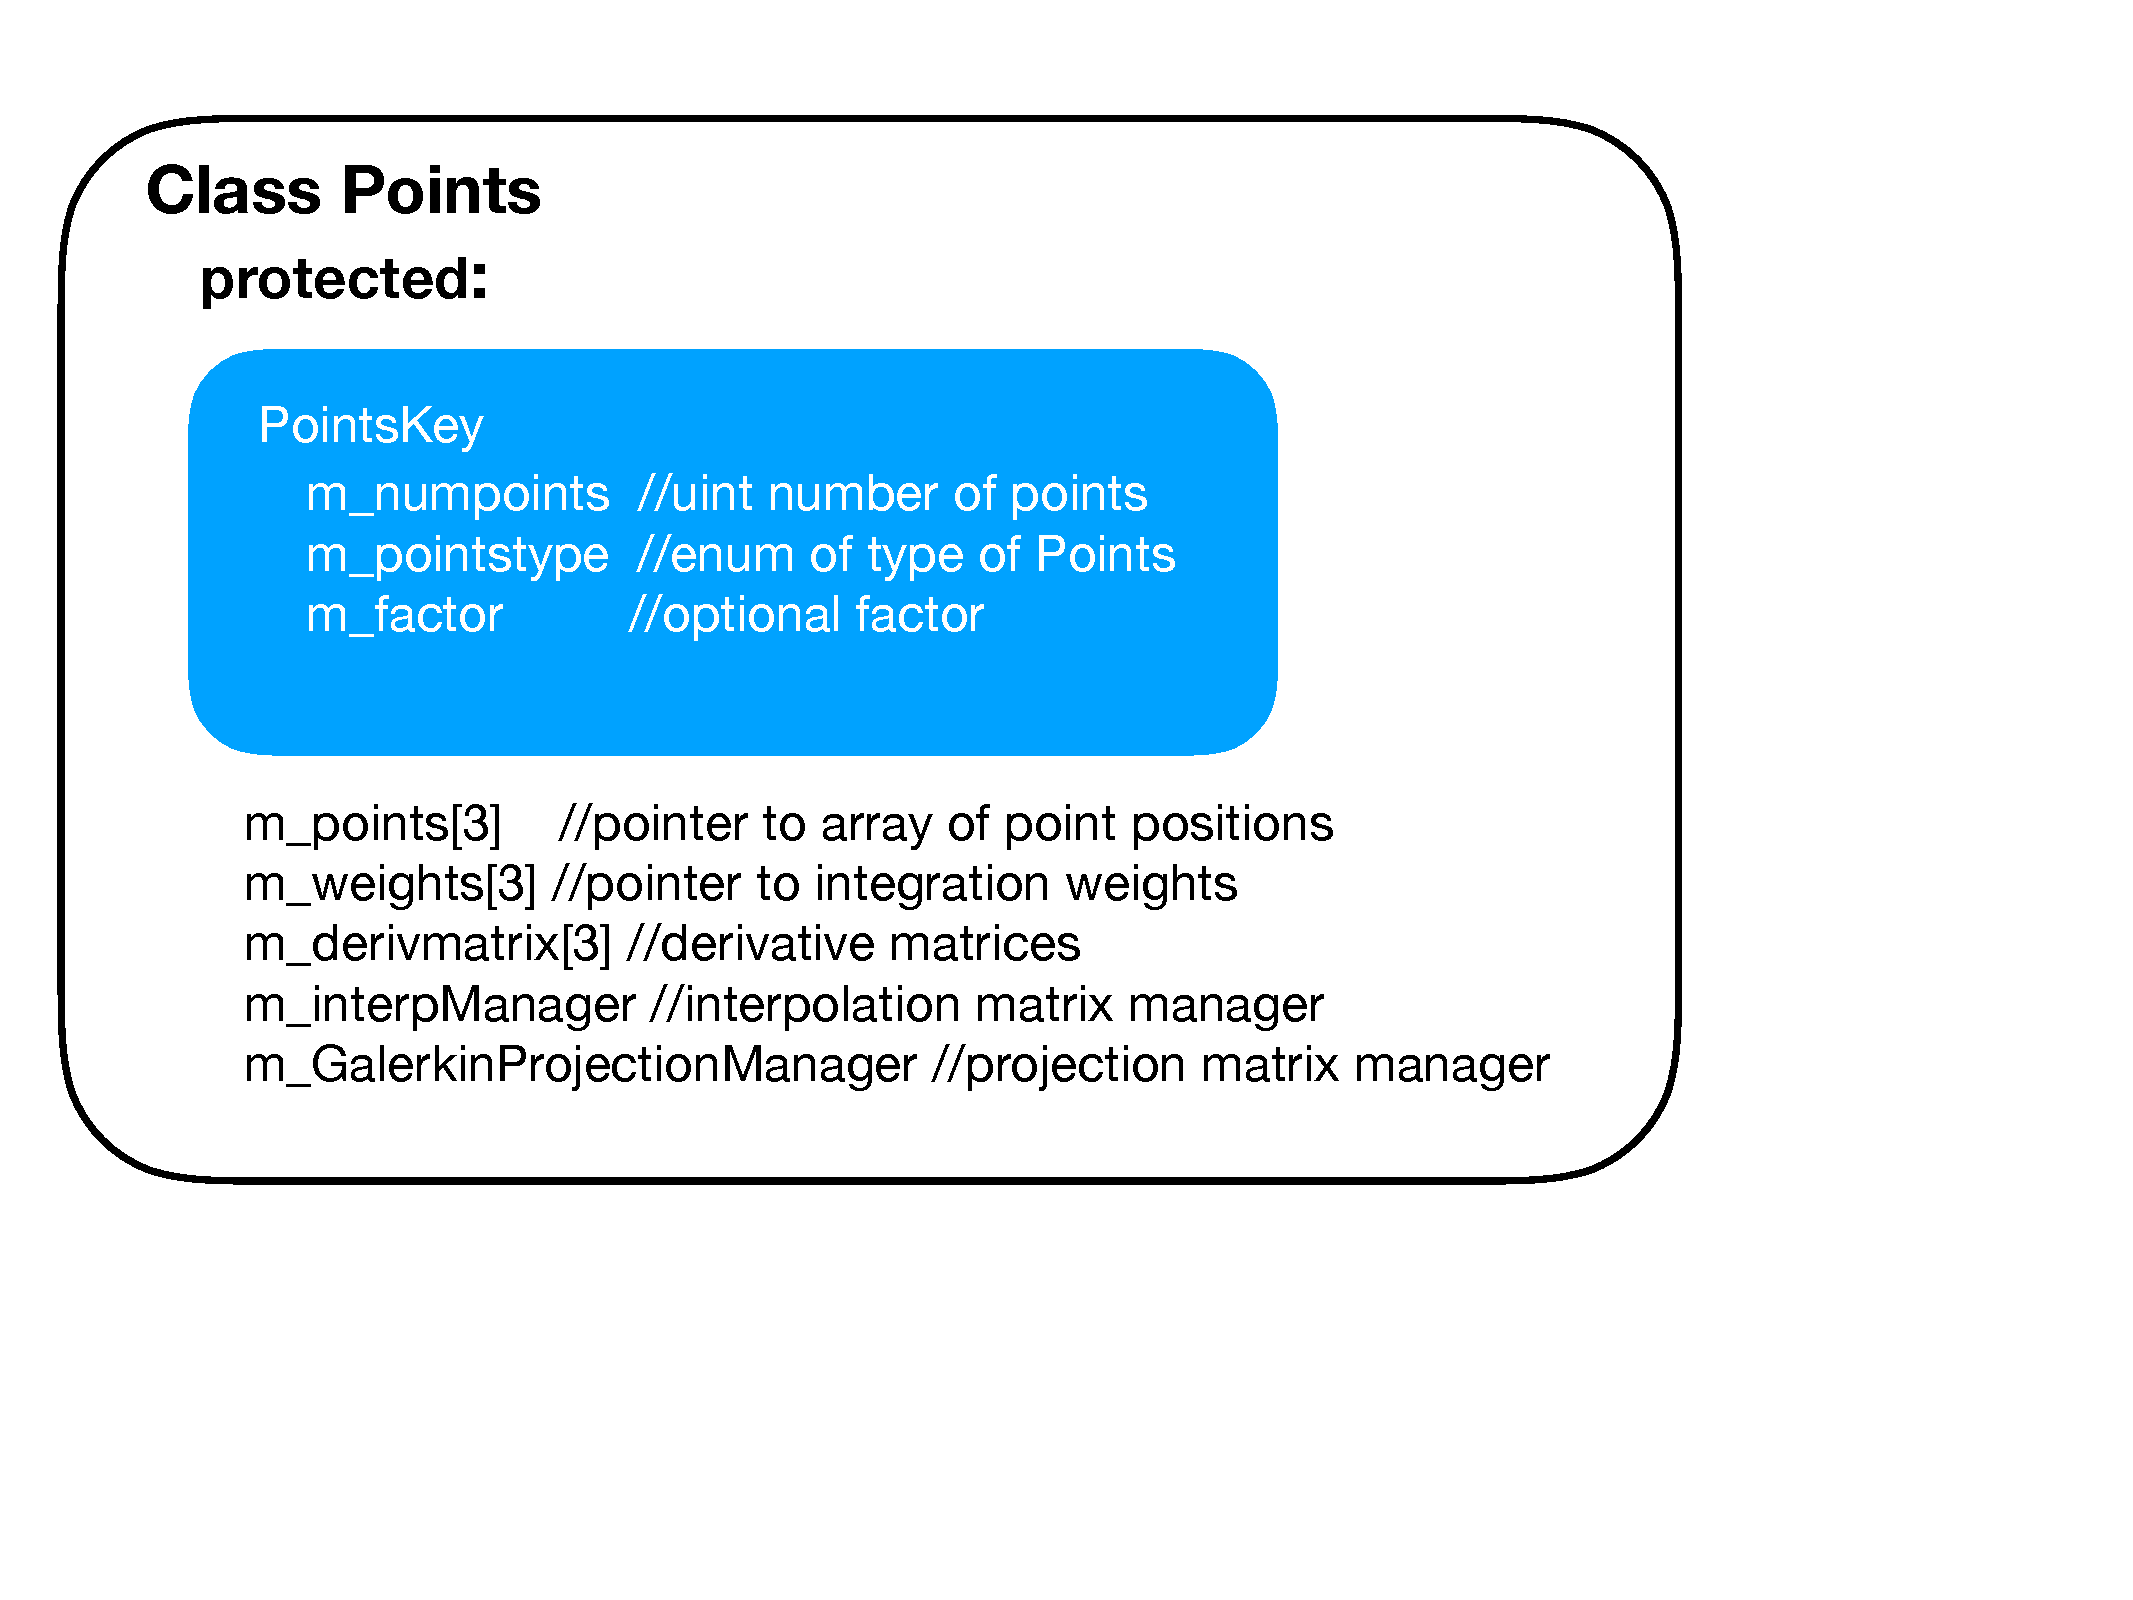
\includegraphics[width=4in]{img/pointsclass.pdf}
\caption{The basic Points class data object.  It consists of a PointsKey (used by a PointsManager) and various other data members needed for point operations.}
\label{foundations:pointsclass}
\end{figure}


The PointsKey object has three basis data members: the number of points, an enum specifying the point distribution, and a optional
scaling factor.  In almost all of {\nek}, only the first two are needed to uniquely specify a collection of points.  The latter variable was
added as part of the extensions of {\nek} to accommodate NekMesh.  As stated above, if you pass a PointsKey to a PointsManager
you will receive back a pointer to a Points object with its various data members populated, among them a PointsKey identifier for the
object.  As can be seen by the diagram, the Points object has a collection (array) of three pointers to point positions.  These three
array pointers allow Points objects to point to 1D, 2D or 3D point positions.  Corresponding to the dimension and associated with each
point position is a weight associated with integration.  This was done to facilitate both non-tensor product and tensor product constructions. 
To demonstrate non-tensor product constructions, consider if you were 
to be dealing with a 2D point set that is natively 2D (that is, not based upon tensor product construction such
as the Electrostatic Points), then the number
of points in the PointsKey would be the size of each array associated with \verb+m_points+, and only one of the \verb+m_weight+ 
arrays (associated with \verb+m_weight[0])+ would be valid such at:

\[
\int_{\Omega_{2D}} f(x_{0},x_{1}) \, dx_0\,dx_1 \approx \sum_{i=0}^{numpoints-1} \omega_i f(z_{0,i},z_{1,i})
\]

\noindent where $z_{0,i}$ and $z_{1,i}$ denote the points associated with \verb+m_points[0][i]+ and \verb+m_points[1][i]+ respectively.
The weights in this case are calculated by routines found in NodalUtils via forming a Vandermonde system, solving for Lagrange
basis functions that pass through a particular set of points, and then integrating those basis functions to obtain weights. 
This operation is done sufficiently often that we will try to spell it out after the Fekete Point paragraph below.  

If one is dealing with a tensor product constructed 2D nodal point set, one would have:

\[
\int_{\Omega_{2D}} f(x_{0},x_{1}) \, dx_0\,dx_1 \approx \sum_{i=0}^{numpoints-1} \left[ \sum_{j=0}^{numpoints-1} \omega_i \omega_j f(z_{0,i},z_{1,j})\right]
\]

\noindent where $z_{0,i}$ and $z_{1,i}$ denote the points associated with \verb+m_points[0][i]+ and \verb+m_points[1][i]+ respectively
and $\omega_i$ and $\omega_j$ are the weights associated with the two coordinate directions respectively.  The tensor product
construction above was implemented in {\nek} assuming we would create derived nodal point sets for quadrilaterals and hexahedron; however,
throughout much of {\nek}, we use the tensor product forms explicitly by specifying 1D point sets in the different directions as needed.
This particular point will become more apparent when you get to reading the Chapter on StdRegions (Chapter \ref{chap:stdregions}).  You will
encounter, for instance, that a Standard Quadrilateral Expansion (StdQuadExp) requires two 1D Point objects denoting the two 
coordinates for integration.  In this case, the number of points and number of weights match up per direction.


\paragraph{Electrostatic Points: }

The Electrostatic (Nodal) Points on the triangle and tetrahedron are based upon the work 
of Hesthaven \cite{Hesthaven98}.  They are an attempt to find the minimizer of a potential energy function based upon
an electrostatic point source analogy, and provide points that correspondingly have low Lebesgue constant.  The point positions
as given in the paper are stored in the files NodalTriElecData.h and NodalTetElecData.h.  
Hesthaven uses a condensed format for the nodal positions which
rely on the symmetries of the points (if you count the points in the file, you will see that fewer points are given than are needed
to span the polynomial space.  For example, for degree one, a single point it given.   This point along with its three-fold symmetries
represent all three points needed to support the linear space).   The routine \verb+CalculatePoints()+ expands the condensed 
format of the points to the full set based upon the one, three (a and b denoting two types of three-symmetries) 
and six symmetries.  Note that the ordering of the nodes
expanded from the file does not respect any particular geometric ordering, so we reorder the points using \verb+NodalPointReorder2d()+,
which reorganizes the points in vertex points, edge points, and then interior points (i.e. a geometric decomposition that aligns more
naturally with the way we organize nodes/modes within {\nek}).  In Figure \ref{foundations:nodeordering} we show an example
of this reordering done for the points needed for expressing a total degree three expansion over a triangle.

\begin{figure}[htb]
\centering
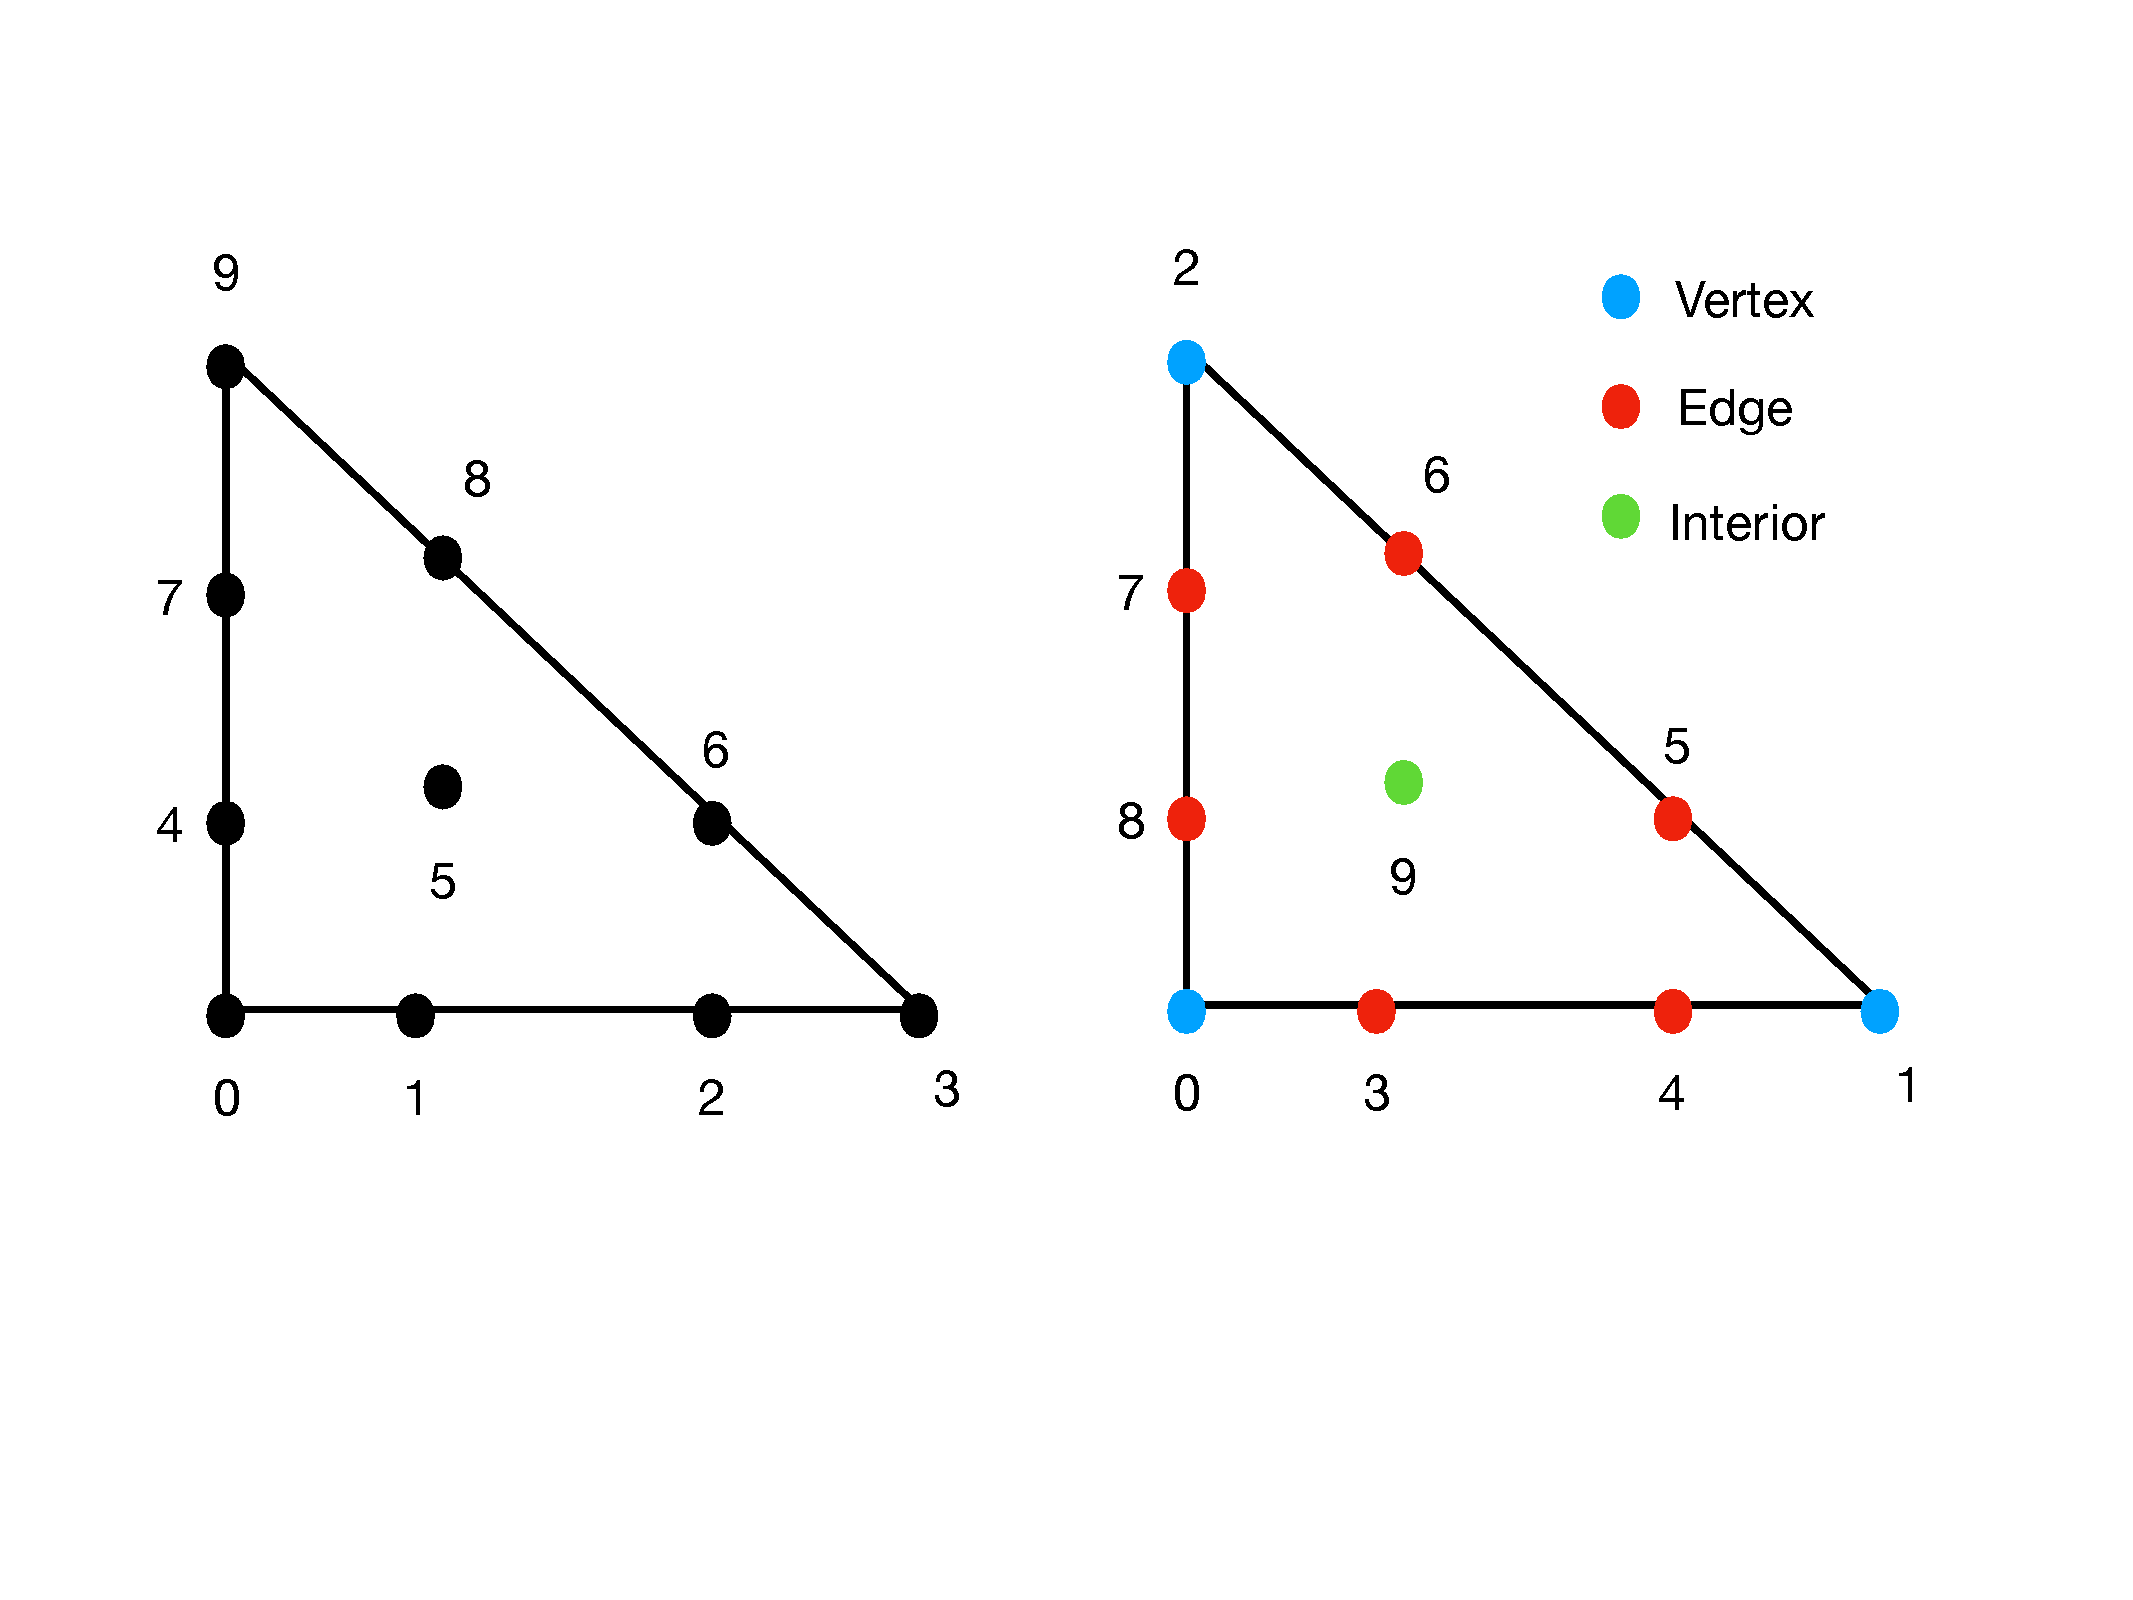
\includegraphics[width=4in]{img/nodeordering.pdf}
\caption{Example of how nodes are reordered to meet a geometric ordering.  On the left, we show the nodal positions that would
be used for building a total degree three polynomial space over a triangle ordered in canonical form.  On the right, we show 
the reordering of those nodes to follow a vertex, edge and interior ordering.  Note that in the case of a tetrahedron, the
ordering would be vertex, edge, face and then interior.}
\label{foundations:nodeordering}
\end{figure}


\paragraph{Fekete Points: }

The Fekete (Nodal) Points on a triangle are based upon the work of Taylor and Wingate \cite{TaylorW99,TaylorWV00},
and are an alternative nodal point distribution on both triangles and tetrahedra. 
As an alternative strategy to the one mentioned above, Taylor and Wingate explicitly attempt to find a point
distribution that minimizes the Lebesgue constant.  For their particular point set, the minimization if over
the Lebesgue function itself (not the electrostatic potential function, which can be viewed as a proxy for this function).  
The point positions as given in the paper are stored in the file NodalTriFeketeData.h and NodalTetFeketeData.h.  
Taylor and Wingate use a condensed format for the nodal positions similar to that used by Hesthaven.

\paragraph{Building Lagrange Interpolating Polynomials: }
One common operation done in both the case of the Electrostatic Points and the Fekete Points is to build the
Lagrange interpolating polynomial associated with a point set.  This is needed, for instance, for computing the integration
weights associated with a particular collection of points (as mentioned above).  This 
operation is done sufficiently often that we will try to spell it out here.  Forming the Lagrange basis functions for a particular
set of points, in particular in 2D and 3D, is non-trivial.  The most common way of arriving at a set of actionable basis functions is
to use a known basis (for which we are able to explicitly write down its form) 
and find the linear combination of those basis functions that yield the Lagrange basis.  For example, let us
assume we are dealing with the set of Electrostatic Points on a triangle.  The number of points, \verb+numpoints+, will
specify the number of ``modes'' (coefficients) we expect to find.  The total degree of the space is given by $N = \frac{(M+1)(M+2)}{2}$
where $N$ is the degree of the polynomials and $M$ is the number of points.  As an example: 
note that when $M=3$, we get $N=1$ -- that is, with three points we can support a polynomial of total 
degree one over a triangle.  Let $\phi_i$ denote a known non-interpolating basis function.  Although not
done in practice, imagine that this is, for instance, a monomial.  In 1D, this would equate to $\phi_i(x) = x^i$, and in
multiple dimensions this would equate to $\phi_i(x,y) = x^{i_1}y^{i_2}$ with some index mapping function $i=\sigma(i_1,i_2)$
that gives us an index ordering.  The total number of basis functions to span our degree $N$ space is given by $M$.
We first form the Vandermonde matrix ${\bf V}$ as follows:


\[
 {\bf V} =  \left[ {\begin{array}{cccc}
   \phi_0(x_{0,0},x_{1,0}) & \phi_1(x_{0,0},x_{1,0}) & \ldots & \phi_N(x_{0,0},x_{1,0}) \\
   \phi_0(x_{0,1},x_{1,1}) & \phi_1(x_{0,1},x_{1,1}) & \ldots & \phi_N(x_{0,1},x_{1,1}) \\
                                        & \vdots & & \\
   \phi_0(x_{0,N},x_{1,N}) & \phi_1(x_{0,N},x_{1,N}) & \ldots & \phi_N(x_{0,N},x_{1,N}) \\
  \end{array} } \right]
\]

\noindent where each row $i$ denotes the evaluation of our $N$ basis functions at a given point $(x_{0,i},x_{1,i})$.
Since we have selected the number of basis functions to be what can be uniquely resolved by our $N$ points, this matrix
is square and invertible.  The conditioning of the matrix is based upon our basis choice; hence we know that monomials 
are not a good choice beyond approximately cubics so in general we use our internal modified basis for this system.
With ${\bf V}$ now available, we can form the linear system:

\[
{\bf V}{\bf c} = {\bf b}
\]

\noindent where ${\bf c}$ is the vector of coefficients and where ${\bf b} = b_i$ is a binary vector where the $i^{th}$ entry is set to one
when finding the coefficients for the $i^{th}$ Lagrange basis function associated with a particular set of points.  For each Lagrange
basis function definition we seek to find, we update the right-hand-side vector and solve the linear system for the set of 
coefficients that denote the combination of our known basis that yields a Lagrange basis function.  Note that since this
operation (of ``inverting" this linear system) must be done for each Lagrange basis function, we can optimize our operations 
by accomplishing LU decomposition on ${\bf V}$ first, which can be done in $\mathcal{O}(N^2)$ operations, and then
each solution for the coefficient vector can be done in $\mathcal{O}(N)$ operations through backsolves.

\paragraph{Finding Integration Weights: }
When the points are related to Gaussian quadrature, the array \verb+m_weights+ will contain
the appropriate Gaussian quadrature weights computed using point and weight routines found in Foundations (our polymath
library functions).  In the case of weights associated with points sets that do not lie at the zeros of Jacobi polynomials, 
we must compute the weights directly based upon Lagrange interpolation through those points.  Although this can
be done in general for any point distribution, we will focus here on evenly-spaced points (note that when one
applies this approach to Chebyshev points, one arrives at Clenshaw-Curtis quadrature \cite{ClenshawC}).
Within {\nek}, given evenly-spaced points on the interval $[-1,1]$ -- if only one point is given,
then the weight is set to $2.0$ denoting a midpoint integration rule; otherwise, the weights are given by
the following expression:

\[
w_j = \int_{-1}^1 \ell_j(\xi)\, d\xi
\]

\noindent where $\ell_j(\xi)$ is the Lagrange basis function defined over an evenly-spaced set of points $\xi_k \in [-1,1]$.
For 2D and 2D nodal point sets (such as Electrostatic and Fekete Points), this same procedure is used.   We first form the
Lagrange interpolating functions via the algorithm given above (using the Vandermonde system), and then for each 
quadrature weight compute the integral of that Lagrange basis function using some known quadrature rule (such as
tensor product quadrature via Duffy transformation; this point will be more easily understood after reading Chapter
\ref{chap:stdregions})




\subsection{Basis}
The second of the two primary data structures in this directory is Basis. 
A basis object consists of a BasisKey and the extra information needed
to facilitate various operations on the basis.  The basis layout of the data 
structure is shown in Figure \ref{foundations:basisclass}.  

\begin{figure}[htb]
\centering
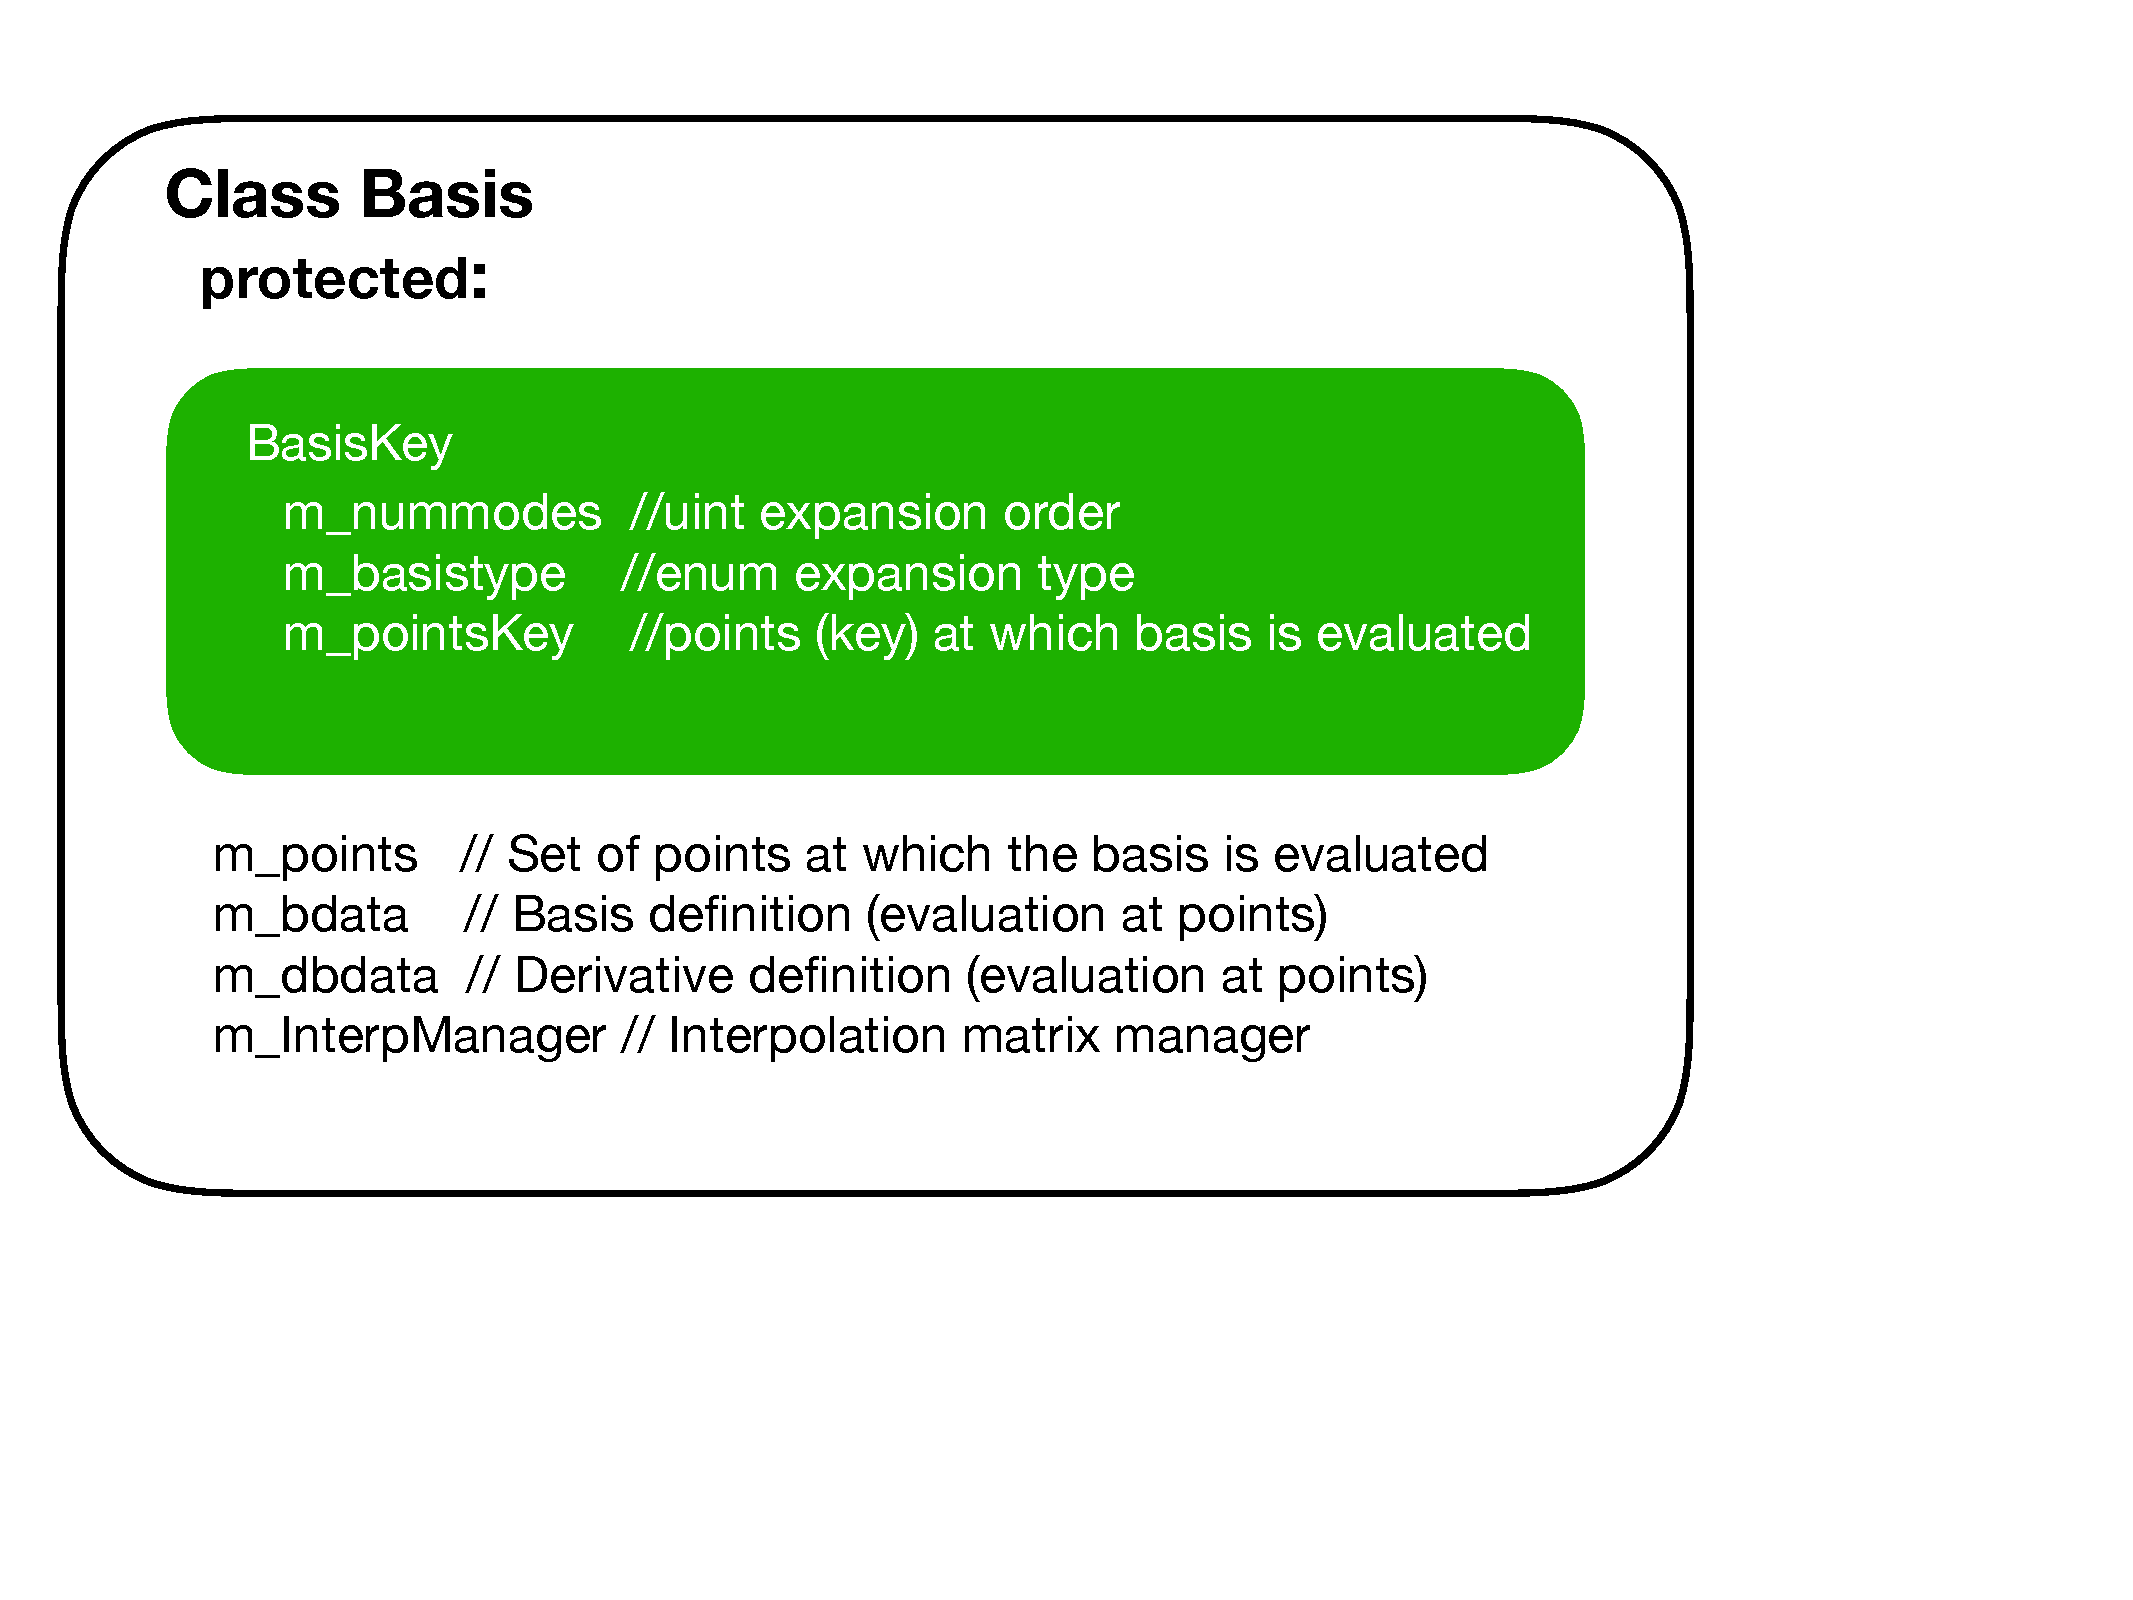
\includegraphics[width=4in]{img/basisclass.pdf}
\caption{The basic Basis class data object.  It consists of a BasisKey (used by a BasisManager) and various other data members needed for point operations.}
\label{foundations:basisclass}
\end{figure}


The Basis
object consists of a BasisKey (which in turn holds a PointsKey), 
a pointer to the positions at which the basis is evaluated and then
arrays which hold the evaluation of the basis (\verb+m_bdata+) and
the evaluation of the derivates of the basis (\verb+m_dbdata+).
The storage layout for these data structures are shown in 
Figure \ref{foundations:basisclass}.  The number of rows is given by 
the number of modes associated with a particular expansion, and the
number of columns is given by the number of points.  These arrays are stored
as contiguous memory to help avoid excessive memory hopping. 
      
\begin{figure}[htb]
\centering
\includegraphics[width=4in]{img/basismemory.pdf}
\caption{Diagram of the basic memory layout of the arrays associated with the basis and its derivatives evaluated at points.}
\label{foundations:basismemory}
\end{figure}

%
%
\section{Interpreter}

This directory contains two files, AnalyticExpressionEvaluator.hpp and AnalyticExpressionEvaluator.cpp, both of which provide
parser and evaluator functionality of analytic expressions.
%
%
\section{Kernel}

This directory contains two files, kernel.h and kernel.cpp, both of which are related to the line-SIAC (L-SIAC) filtering \cite{sanchez2016multi,jallepalli2017treatment} of FEM solutions.
SIAC filtering takes the form:

$$
u^*(x) = \int_{-\infty}^{\infty} K_H\left(\frac{\xi - x}{H}\right) u_h(\xi) \, d\xi
$$

\noindent where $u_h$ denotes the FEM (continuous Galkerkin or discontinuous Galerkin) solution and $K_H$ represents a kernel function:

$$
K_H(x) = \frac{1}{H} \sum_{\gamma = 0}^M c_\gamma \psi\left(\frac{x}{H} - \zeta_\gamma \right).
$$

In this expression, the functions $\psi(x)$ are B-Splines.  The two kernel files in this directory provide all the tools needed to construct the B-Spline functions and the kernel function described above.
%
%
\section{Linear Algebra}

This directory contains files related to linear algebra operations.  Files such as NekMatrix, BlockMatrix and NekLinearSystem are fundamental to many of the operations we do within {\nek}.
These files represent our attempt to encapsulate linear algebra operations in a way that make sense from the programmer perspective but for which we do not loose efficiency.  As can be seen in these
routines and throughout the code, we rely heavily on BLAS (Basic Linear Algebra Subroutines).

\begin{center}
\begin{tabular}{|c | c | c |} \hline
Arpack.hpp &	blas.cpp & Blas.hpp \\ \hline
BlasArray.hpp	& BlockMatrix.cpp & BlockMatrix.hpp \\ \hline
CanGetRawPtr.hpp & ExplicitInstantiation.h & Lapack.hpp \\ \hline
MatrixBase.cpp	& MatrixBase.hpp	 & MatrixFuncs.cpp	\\ \hline
MatrixFuncs.h	& MatrixOperations.cpp & MatrixOperations.hpp \\ \hline
MatrixStorageType.h & MatrixType.h & MatrixVectorMultiplication.cpp	\\ \hline
NekLinAlgAlgorithms.hpp	& NekLinSys.hpp	& NekLinSysIter.cpp \\ \hline
NekLinSysIter.h &  NekLinSysIterCG.cpp & NekLinSysIterCG.h \\ \hline
NekLinSysIterGMRES.cpp & NekLinSysIterGMRES.h & NekMatrix.hpp \\ \hline
NekMatrixFwd.hpp & NekNonlinSys.cpp & NekNonlinSys.h \\ \hline
NekNonlinSysNewton.cpp & NekNonlinSysNewton.h & NekPoint.hpp \\ \hline
NekTypeDefs.hpp &  NekVector.cpp & NekVector.hpp \\ \hline
NekVectorFwd.hpp & NistSparseDescriptors.hpp & PointerWrapper.h \\ \hline
ScaledMatrix.cpp & ScaledMatrix.hpp & SparseDiagBlkMatrix.cpp \\ \hline
SparseDiagBlkMatrix.hpp & SparseMatrix.cpp & SparseMatrix.hpp \\ \hline
SparseMatrixFwd.hpp & SparseUtils.cpp & SparseUtils.hpp \\ \hline
StandardMatrix.cpp & StandardMatrix.hpp & StorageSmvBsr.cpp \\ \hline
StorageSmvBsr.hpp & TransF77.hpp & \\ \hline
\end{tabular}
\end{center}

%
%
\section{Memory}

This directory contains three files, NekMemoryManager.hpp, ThreadSpecificPools.hpp and ThreadSpecificPools.cpp.
The strategy used within {\nek} was to preallocate a pool of arrays that could be used for various operations and then
released back to the pool.  This idea came about through profiling of the code early on -- noticing that the new/delete
operation of lots of small arrays used for temporary calculations was greatly slowing down the code.  Like with our manager
idea, we decided to invest in having a memory pool object what preallocated blocks of memory that could be requested and
then returned back to the pool.

If {\nek} is compiled with \verb+NEKTAR_MEMORY_POOL_ENABLED+, the MemoryManager
allocates from thread specific memory pools for small objects. Large objects are managed with the 
system supplied new/delete. These memory pools provide faster allocation and deallocation
of small objects (particularly useful for shared pointers which
allocate many 4 byte objects).

All memory allocated from the memory manager must be returned
to the memory manager.  Calling delete on memory allocated from the
manager will likely cause undefined behavior.  A particularly subtle
violation of this rule occurs when giving memory allocated from the
manager to a shared pointer.

%
%
\section{Polylib}

This directory contains polylib.h and polylib.cpp.  These files contain foundational routines used for computing various operations related to Jacobi polynomials.
The following abbreviations are used throughout the file:

\begin{itemize}
\item z   --   Set of collocation/quadrature points
%
\item w   --   Set of quadrature weights
%
\item D   --   Derivative matrix
%
\item h   --   Lagrange Interpolant
%
\item I    --   Interpolation matrix
%
\item g   --   Gauss
%
\item	 k   --   Kronrod
%
\item  gr  --   Gauss-Radau
%
\item  gl  --   Gauss-Lobatto
%
\item  j    --   Jacobi
%
\item  m  --   point at minus 1 in Radau rules
%
\item  p  --   point at plus  1 in Radau rules
\end{itemize}


\paragraph{Points and Weights: }  The following routines are used to compute points and weights:

\begin{itemize}
\item zwgj    --   Compute Gauss-Jacobi points and weights
%
\item zwgrjm  --   Compute Gauss-Radau-Jacobi points and weights ($z=-1$)
%
\item zwgrjp  --  Compute Gauss-Radau-Jacobi  points and weights ($z=1$)
%
\item zwglj    --  Compute Gauss-Lobatto-Jacobi points and weights
%
\item	zwgk   --  Compute Gauss-Kronrod-Jacobi points and weights
%
\item	zwrk   --  Compute Radau-Kronrod points and weights
%
\item	zwlk  --  Compute Lobatto-Kronrod points and weights
%
\item	 JacZeros  --  Compute Gauss-Jacobi points and weights
\end{itemize}

\paragraph{Derivative Matrices: } The following routines are used to compute derivative matrices:

\begin{itemize}
\item  Dgj  --   Compute Gauss-Jacobi  derivative matrix
%
\item Dgrjm --   Compute Gauss-Radau-Jacobi  derivative matrix ($z=-1$)
%
\item  Dgrjp  --  Compute Gauss-Radau-Jacobi  derivative matrix ($z=1$)
%
\item  Dglj  --  Compute Gauss-Lobatto-Jacobi derivative matrix
\end{itemize}

\paragraph{Lagrange Interpolants: } The following routines are used to compute Lagrange interpolation matrices:

\begin{itemize}
\item hgj  --  Compute Gauss-Jacobi  Lagrange interpolants
%
\item hgrjm --  Compute Gauss-Radau-Jacobi  Lagrange interpolants ($z=-1$)
%
\item hgrjp --   Compute Gauss-Radau-Jacobi  Lagrange interpolants ($z=1$)
%
\item hglj  --   Compute Gauss-Lobatto-Jacobi Lagrange interpolants
\end{itemize}

\paragraph{Interpolation Operators: } The following routines are used to compute various interpolation operators:

\begin{itemize}
\item Imgj  --  Compute interpolation operator gj->m
%
\item Imgrjm  --  Compute interpolation operator grj->m ($z=-1$)
%
\item Imgrjp  --  Compute interpolation operator grj->m ($z=1$)
%
\item Imglj  --  Compute interpolation operator glj->m
\end{itemize}

\paragraph{Polynomial Evaluation: } The following routines are used to evaluate Jacobi polynomials.

\begin{itemize}
 \item jacobfd  --   Returns value and derivative of Jacobi polynomial at point z
%
 \item jacobd  --    Returns derivative of Jacobi polynomial at point z (valid at $z=-1,1$)
\end{itemize}
       
%
%
\section{Time Integration}

This directory consists of the following files:


\begin{center}
\begin{tabular}{|c | c | } \hline
TimeIntegrationScheme.h & TimeIntegrationScheme.cpp \\ \hline 
TimeIntegrationGLM.h & TimeIntegrationGLM.cpp \\ \hline
*TimeIntegrationSchemes.h & Specific GLM schemes, e.g. AB, RK, IMEX, etc. \\ \hline
TimeIntegrationFIT.h & TimeIntegrationFIT.cpp \\ \hline
\end{tabular}
\end{center}

The original time-stepping interface (found in the parent class
TimeIntegrationScheme) where implemented by Vos et al. \cite{Vostime}
and a detailed explanation of the mathematics and computer science
concepts are provided there.  After the original implementation,
Cantwell et al. extended Vos' original work by adding the
time-stepping routines into a factory pattern (found in the child
class TimeIntegrationGLM). The GLM schemes have been further
compartmentalized into specific schemes covering both traditional and
exponential schemes. More recently Fractional-in-time schemes have
been added (found in the child class TimeIntegrationFIT). 

\subsection{General Linear Methods}
General linear methods (GLMs) can be considered as the generalization
of a broad range of different numerical methods for ordinary
differential equations.  They were introduced by Butcher and they
provide a unified formulation for traditional methods such as the
Runge-Kutta methods and the linear multi-step methods such as
Adams-Bashforth.  From an implementation point of view, this means
that all these numerical methods can be abstracted in a similar
way. As this allows a high level of generality, it is chosen in {\nek}
to cast all time integration schemes in the framework of general
linear methods.

For background information about general linear methods, please consult
\cite{Bu06}.

\subsubsection{Introduction}
The standard initial value problem can written in the form
\begin{align*}
\frac{d\boldsymbol{y}}{dt} = \boldsymbol{f}(t,\boldsymbol{y}),\quad
\boldsymbol{y}(t_0)=\boldsymbol{y}_0
\end{align*}
where $\boldsymbol{y}$ is a vector containing the variable (or an
array of array containing the variables).

In the formulation of general linear methods, it is more convenient to consider
the ODE in autonomous form, i.e.
\begin{align*}
\frac{d\boldsymbol{\hat{y}}}{dt}=\boldsymbol{\hat{f}}(\boldsymbol{\hat{y}}),\quad
\boldsymbol{\hat{y}}(t_0)= \boldsymbol{\hat{y}}_0.
\end{align*}

\subsubsection{Formulation}
Suppose the governing differential equation is given in autonomous form, the
$n^{th}$ step of the GLM comprising
\begin{itemize}
\item $r$ steps (as in a multi-step method)
\item $s$ stages (as in a Runge-Kutta method)
\end{itemize}
is formulated as:
\begin{align*}
\boldsymbol{Y}_i &= \Delta
t\sum_{j=0}^{s-1}a_{ij}\boldsymbol{F}_j+\sum_{j=0}^{r-1}u_{ij}\boldsymbol{\hat{y}}_{j}^{[n-1]},
\qquad i=0,1,\ldots,s-1 \\
\boldsymbol{\hat{y}}_{i}^{[n]}&=\Delta
t\sum_{j=0}^{s-1}b_{ij}\boldsymbol{F}_j+\sum_{j=0}^{r-1}v_{ij}
\boldsymbol{\hat{y}}_{j}^{[n-1]}, \qquad i=0,1,\ldots,r-1
\end{align*}
where $\boldsymbol{Y}_i$ are referred to as the stage values and
$\boldsymbol{F}_j$ as the stage derivatives. Both quantities are
related by the differential equation:
\begin{align*}
\boldsymbol{F}_i = \boldsymbol{\hat{f}}(\boldsymbol{Y}_i).
\end{align*}

The matrices $A=[a_{ij}]$, $U=[u_{ij}]$,
$B=[b_{ij}]$, $V=[v_{ij}]$ are characteristic of a
specific method. Each scheme can then be uniquely defined by a partitioned
$(s+r)\times(s+r)$ matrix
\begin{align*}
\left[
\begin{array}{cc}
  A & U\\
  B & V \end{array}\right]
\end{align*}


\subsubsection{Matrix notation}
Adopting the notation:
\begin{align*}
\boldsymbol{\hat{y}}^{[n-1]}= \left[\begin{array}{c}
\boldsymbol{\hat{y}}^{[n-1]}_0\\
\boldsymbol{\hat{y}}^{[n-1]}_1\\
\vdots\\
\boldsymbol{\hat{y}}^{[n-1]}_{r-1}
\end{array}\right],\quad \boldsymbol{\hat{y}}^{[n]}= \left[\begin{array}{c}
\boldsymbol{\hat{y}}^{[n]}_0\\
\boldsymbol{\hat{y}}^{[n]}_1\\
\vdots\\
\boldsymbol{\hat{y}}^{[n]}_{r-1}
\end{array}\right],\quad \boldsymbol{Y}= \left[\begin{array}{c}
\boldsymbol{Y}_0\\
\boldsymbol{Y}_1\\
\vdots\\
\boldsymbol{Y}_{s-1}
\end{array}\right],\quad \boldsymbol{F}= \left[\begin{array}{c}
\boldsymbol{F}_0\\
\boldsymbol{F}_1\\
\vdots\\
\boldsymbol{F}_{s-1}
\end{array}\right]\quad
\end{align*}
the general linear method can be written more compactly in the following form:
\begin{align*}
\left[ \begin{array}{c} \boldsymbol{Y}\\
\boldsymbol{\hat{y}}^{[n]}
\end{array}\right] = \left[ \begin{array}{cc} A\otimes I_N & U\otimes I_N \\
B\otimes I_N & V\otimes I_N \end{array}\right] \left[ \begin{array}{c} \Delta
t\boldsymbol{F}\\
\boldsymbol{\hat{y}}^{[n-1]}
\end{array}\right]
\end{align*}
where $I_N$ is the identity matrix of dimension $N\times N$.


\subsubsection{General Linear Methods in Nektar++}
Although the GLM is essentially presented for ODE's in its autonomous form, in
Nektar++ it will be used to solve ODE's formulated in non-autonomous form.
Given the ODE,
\begin{align*}
\frac{d\boldsymbol{y}}{dt}=\boldsymbol{f}(t,\boldsymbol{y}),\quad
\boldsymbol{y}(t_0)=\boldsymbol{y}_0
\end{align*}
a single step of GLM can then be evaluated in the following way:
\begin{itemize}
\item \textbf{input}

$\boldsymbol{y}^{[n-1]}$, \emph{i.e.} the $r$
    subvectors comprising $\boldsymbol{y}^{[n-1]}_i$ -
    $t^{[n-1]}$, \emph{i.e.} the equivalent of
    $\boldsymbol{y}^{[n-1]}$ for the time variable $t$.

\item \textbf{step 1}: The stage values $\boldsymbol{Y}_i$,
$\boldsymbol{T}_i$ and the stage derivatives
$\boldsymbol{F}_i$ are calculated through the relations:
\begin{enumerate}
\item $\boldsymbol{Y}_i = \Delta
    t\sum_{j=0}^{s-1}a_{ij}\boldsymbol{F}_j+\sum_{j=0}^{r-1}u_{ij}\boldsymbol{y}_{j}^{[n-1]},
    \qquad i=0,1,\ldots,s-1$
\item $T_i\ =\ \Delta
    t\sum_{j=0}^{s-1}a_{ij}+\sum_{j=0}^{r-1}u_{ij}t_{j}^{[n-1]}, \qquad
    i=0,1,\ldots,s-1$
\item $\boldsymbol{F}_i\ =\
    f(T_i,\boldsymbol{Y}_i), \qquad i=0,1,\ldots,s-1$
\end{enumerate}

\item \textbf{step 2}: The approximation at the new time level
$\boldsymbol{y}^{[n]}$ is calculated as a linear combination of the
stage derivatives $\boldsymbol{F}_i$ and the input vector
$\boldsymbol{y}^{[n-1]}$. In addition, the time vector
$t^{[n]}$ is also updated

\begin{enumerate}
\item $\boldsymbol{y}_{i}^{[n]} = \Delta
    t\sum_{j=0}^{s-1}b_{ij}\boldsymbol{F}_j+\sum_{j=0}^{r-1}v_{ij}\boldsymbol{y}_{j}^{[n-1]},
    \qquad i=0,1,\ldots,r-1$
\item $t_{i}^{[n]}\ =\ \Delta
    t\sum_{j=0}^{s-1}b_{ij}+\sum_{j=0}^{r-1}v_{ij}t_{j}^{[n-1]}, \qquad
    i=0,1,\ldots,r-1$
\end{enumerate}

\item \textbf{output}
\begin{enumerate}
\item $\boldsymbol{y}^{[n]}$, i.e. the $r$ subvectors
    comprising $\boldsymbol{y}^{[n]}_i$.
    $\boldsymbol{y}^{[n]}_0$ corresponds to the actual approximation
    at the new time level.
\item $t^{[n]}$ where $t^{[n]}_0$ is equal to the new time
    level $t+\Delta t$.
\end{enumerate}
\end{itemize}

For a detailed description of the formulation and a deeper insight of the
numerical method see \cite{Vostime}.


\subsubsection{Types of time Integration Schemes}
Nektar++ contains various classes and methods which implement the
concept of GLMs. This toolbox is capable of numerically solving the
generalised ODE using a broad range of different time-stepping
methods. We distinguish the following types of general linear methods:
\begin{itemize}
\item \textbf{Formally Explicit Methods}: These types of methods are
  considered explicit from an ODE point of view. They are
  characterised by a lower triangular coefficient matrix $A$, ''i.e.''
  $a_{ij} = 0$ for $j\geq i$. To avoid confusion, we make a further
  distinction:
  \begin{itemize}
    \item \textbf{direct explicit method}: Only forward operators are
      required.
    \item \textbf{indirect explicit method}: The inverse operator is
      required.
  \end{itemize}
  \item \textbf{Diagonally Implicit Methods}: Compared to explicit
    methods, the coefficient matrix $A$ has now non-zero entries on
    the diagonal.  This means that each stage value depend on the
    stage derivative at the same stage, requiring an implicit
    step. However, the calculation of the different stage values is
    still uncoupled. Best known are the DIRK schemes.
  \item \textbf{IMEX schemes}: These schemes support the concept of
    being able to split right hand forcing term into an explicit and
    implicit component. This is useful in advection diffusion type
    problems where the advection is handled explicitly and the
    diffusion is handled implicit.
  \item \textbf{Fully Implicit Methods}: The coefficient matrix has a
    non-zero upper triangular part. The calculation of all stages
    values is fully coupled.
  \item \textbf{Exponential Methods}: A forward Euler method has been
    extended to the exponential setting. These types of methods are
    considered explicit from an ODE point of view. They are
    characterized by a coefficient matrix of exponential values for
    each variable. Two schemes have been implemented:
  \begin{itemize}
    \item \textbf{Lawson-Euler explicit method}: $y_n =
      \varphi_0(z)N(y_{n-1},t_{n-1}) + \varphi_0(z)y_{n-1}$
    \item \textbf{N{\o}rsett-Euler explicit method}: $y_n =
      \varphi_1(z)N(y_{n-1},t_{n-1}) + \varphi_0(z)y_{n-1}$
  \end{itemize}
where $\varphi_0(z) = e^{z}$ for $k = 0$, $\varphi_{k}(z) =
\frac{\varphi_{k-1}(z) - \varphi_{k-1}(0)}{z}$ for $k \geq 1$.
\end{itemize}

The aim in {\nek} is to fully support the first three types of GLMs.
Fully implicit methods are currently not implemented. {\nek} also
fully supports Exponential Methods using GLMs.


\subsection{Fractional-in-time Integration Schemes}

In addition to the GLMs {\nek} also supports fractional methods:
\begin{itemize}
  \item \textbf{Fractional-in-time Methods}: A fast convolution
    algorithm for computing solutions to (Caputo) time-fractional
    differential equations. This is an explicit solver that expresses
    the solution as an integral over a Talbot curve, which is
    discretized with quadrature. First-order quadrature is currently
    implemented (Soon be expanded to forth order).
\end{itemize}

The Fractional methods follow the same paradigm as the GLMs, that is
both have the same parent class and as such are used in a similar
manner.

\subsection{Usage}
The goal of abstracting the concept of general linear methods and
fractional methods is to provide users with a single interface for
time-stepping, independent of the chosen method. The classes tree
allows the user to numerically integrate ODE's using high-order
complex schemes, as if it was done using the Forward-Euler method.
Switching between time-stepping schemes is as easy as changing a
parameter in an input file.

In the already implemented solvers the time-integration schemes have
been set up according to the nature of the equations.  For example the
incompressible Navier-Stokes equations solver allows the use of three
different Implicit-Explicit time-schemes if solving the equations with
a splitting-scheme.  This is because this kind of scheme has an
explicit and an implicit operator that combined solve the ODE's
system.

Once aware of the problem's nature and implementation, the user can
easily switch between some (depending on the problem) of the following
time-integration schemes:

\begin{center}
\footnotesize
\begin{tabular}{p{2.5cm}p{1cm}p{10cm}}
\toprule
Method         & Variant & Order / Free Parameters \\
ForwardEuler   &      & Forward-Euler scheme\\
BackwardEuler  &      & Backward-Euler scheme\\

AdamsBashforth &      & Adams-Bashforth Forward multi-step scheme of order 1-4\\

AdamsMoulton   &      & Adams-Moulton Forward multi-step scheme of order 1-4\\

BDFImplicit    &      & BDF multi-step implicit scheme of order 1-4\\

RungeKutta     &      & Runge-Kutta multi-stage explicit scheme of
                        order 1-5, (2 - midpoint, 3 - Ralston's, 4 - Classic)\\

RungeKutta     & SSP  & Strong Stability Preserving (SSP) variant of
                        the RungeKutta multi-stage explicit scheme of
                        order 1-3\\

DIRK           &      & Diagonally Implicit Runge-Kutta (DIRK) scheme of
                        order 2-3\\

CNAB           &      & Crank-Nicolson-Adams-Bashforth (CNAB) of order 2\\

MCNAB          &      & Modified Crank-Nicolson-Adams-Bashforth (MCNAB)
                        of order 2\\

IMEX           &      & Implicit-Explicit (IMEX) scheme using Backward
                        Different Formula Extrapolation of order 1-4\\

IMEX           & Gear & IMEX Gear variant of order 2\\

IMEX           & dirk & IMEX DIRK variant with free parameters (s, sigma), 
                        where s is the number of implicit stage schemes,
                        sigma is the number of explicit stage scheme and
                        p is the combined order of the scheme.\\

               & dirk & Forward-Backward Euler, first order, free parameters (1,1)\\
               & dirk & Forward-Backward Euler, first order, free parameters (1,2)\\
               & dirk & Implicit-Explicit Midpoint, second order, free parameters (1,2)\\
               & dirk & L-stable, two stage, second order, free parameters (2,2)\\
               & dirk & L-stable, two stage, second order, free parameters (2,3)\\
               & dirk & L-stable, two stage, third order, free parameters (2,3)\\
               & dirk & L-stable, three stage, third order, free parameters (3,4)\\
               & dirk & L-stable, four stage, third order, free parameters (4,4)\\

EulerExponential & Lawson  & Exponential Euler scheme using the
                             Lawson variant of order 1 \\

                  & Norsett & Exponential Euler scheme using the
                              Norsett variant of order 1-4
                              (Higher order not yet properly seeded) \\

FractionalInTime  &         & Fractional-in-time scheme of order 1-4
                              (Higher order not yet properly seeded) \\
                    
\bottomrule
\end{tabular}
\end{center}

Note: in many cases the first order schemes reduce to either a forward
or backward Euler scheme.

{\nek} input file for your problem will ask you for the string
corresponding the time-stepping scheme you want to use, the order, and
optionally the variant and free parameters. In addition, parameters
that define your integration in time, the time-step and number of
steps or final time. For example:\\
\begin{lstlisting}[style=XMLStyle]
<SOLVERINFO>
   <I PROPERTY="EQTYPE" VALUE="UnsteadyNavierStokes" />
   <I PROPERTY="SolverType" VALUE="VelocityCorrectionScheme" />
   <I PROPERTY="AdvectionForm" VALUE="Convective" /> 
   <I PROPERTY="Projection" VALUE="Galerkin" /> 
   <I PROPERTY="TimeIntegrationMethod" VALUE="IMEX" />
   <I PROPERTY="TimeIntegrationVariant" VALUE="dirk" />
   <I PROPERTY="TimeIntegrationOrder" VALUE="2" />
   <I PROPERTY="TimeIntegrationFreeParameters" VALUE="2 3" />
 </SOLVERINFO>
 
 <PARAMETERS>
   <P> TimeStep = 0.001 </P> 
   <P> NumSteps = 1000 </P> 
   <P> Kinvis = 1 </P>
</PARAMETERS>
\end{lstlisting}

The old schema which specifies the method, variant, order, and free
parameters as a single string can still be utilized as it has not been
deprecated.

\begin{center}
\footnotesize
\begin{tabular}{p{4cm}p{10cm}}
\toprule
AdamsBashforthOrder1 & Adams-Bashforth Forward multi-step scheme of order 1\\
AdamsBashforthOrder2 & Adams-Bashforth Forward multi-step scheme of order 2\\
AdamsBashforthOrder3 & Adams-Bashforth Forward multi-step scheme of order 3\\
AdamsBashforthOrder4 & Adams-Bashforth Forward multi-step scheme of order 4\\
AdamsMoultonOrder1   & Adams-Moulton Forward multi-step scheme of order 1\\
AdamsMoultonOrder2   & Adams-Moulton Forward multi-step scheme of order 2\\
AdamsMoultonOrder3   & Adams-Moulton Forward multi-step scheme of order 3\\
AdamsMoultonOrder4   & Adams-Moulton Forward multi-step scheme of order 4\\
BDFImplicitOrder1    & BDF multi-step scheme of order 1 (implicit)\\
BDFImplicitOrder2    & BDF multi-step scheme of order 2 (implicit)\\
RungeKutta5          & Runge-Kutta multi-stage scheme 5th order explicit\\
ClassicalRungeKutta4 & Runge-Kutta multi-stage scheme 4th order explicit (old name)\\
RungeKutta2          & Classical RungeKutta2 method (new name for Midpoint)\\
RungeKutta3\_SSP     & Nonlinear SSP RungeKutta3 explicit\\
RungeKutta2\_ImprovedEuler & Improved RungeKutta2 explicit (old name meaning Heun's method)\\
RungeKutta2\_SSP     & Nonlinear SSP RungeKutta2 explicit (surrogate for RungeKutta2\_ImprovedEuler)\\
ForwardEuler         & Forward-Euler scheme\\
BackwardEuler        & Backward Euler scheme\\
IMEXOrder1           & IMEX 1st order scheme using Euler Backwards Euler
                       Forwards \\
IMEXOrder2           & IMEX 2nd order scheme using Backward Different Formula \&
                       Extrapolation\\
IMEXOrder3           & IMEX 3rd order scheme using Backward Different Formula \&
                       Extrapolation\\
IMEXOrder4           & IMEX 4rd order scheme using Backward Different Formula \&
                       Extrapolation\\
DIRKOrder2           & Diagonally Implicit Runge-Kutta scheme of order 2\\
DIRKOrder3           & Diagonally Implicit Runge-Kutta scheme of order 3\\
CNAB                 & Crank-Nicolson-Adams-Bashforth Order 2 (CNAB)\\
IMEXGear             & IMEX Gear Order 2\\
MCNAB                & Modified Crank-Nicolson-Adams-Bashforth Order 2 (MCNAB)\\
IMEXdirk\_1\_1\_1    & Forward-Backward Euler, first order IMEX DIRK(1,1,1)\\
IMEXdirk\_1\_2\_1    & Forward-Backward Euler, first order IMEX DIRK(1,2,1)\\
IMEXdirk\_1\_2\_2    & Implicit-Explicit Midpoint, second order IMEX DIRK(1,2,2)\\
IMEXdirk\_2\_2\_2    & L-stable, two stage, second order IMEX DIRK(2,2,2)\\
IMEXdirk\_2\_3\_2    & L-stable, two stage, second order IMEX DIRK(2,3,2)\\
IMEXdirk\_2\_3\_3    & L-stable, two stage, third order IMEX DIRK(2,3,3)\\
IMEXdirk\_3\_4\_3    & L-stable, three stage, third order IMEX DIRK(3,4,3)\\
IMEXdirk\_4\_4\_3    & L-stable, four stage, third order IMEX DIRK(4,4,3)\\
\bottomrule
\end{tabular}
\end{center}

{\nek} input file for your problem will ask you just the string
corresponding the time-stepping scheme you want to use (between
quotation marks in the previous list).  In addition, parameters that
define your integration in time, the time-step and number of steps or
final time. For example:\\
\begin{lstlisting}[style=XMLStyle]
<SOLVERINFO>
   <I PROPERTY="EQTYPE" VALUE="UnsteadyNavierStokes" />
   <I PROPERTY="SolverType" VALUE="VelocityCorrectionScheme" />
   <I PROPERTY="AdvectionForm" VALUE="Convective" /> 
   <I PROPERTY="Projection" VALUE="Galerkin" /> 
   <I PROPERTY="TimeIntegrationMethod" VALUE="IMEXdirk_2_3_2" />
 </SOLVERINFO>
 
 <PARAMETERS>
   <P> TimeStep = 0.001 </P> 
   <P> NumSteps = 1000 </P> 
   <P> Kinvis = 1 </P>
</PARAMETERS>
\end{lstlisting}


\subsection{Implementation of a time-dependent problem}
In order to implement a new solver which takes advantage of the
time-integration class in {\nek}, two main ingredients are required:
\begin{itemize}
\item A main files in which the time-integration of you ODE's system is
initialized and performed.
\item A class representing the spatial discretization of your problem, which
reduces your system of PDE's to a system of ODE's.
\end{itemize}

Your pseudo-main file, where you actually loop over the time steps, will look
like
\begin{lstlisting}[style=C++Style]
NekDouble timestep    = 0.1; 
NekDouble time        = 0.0; 
int NumSteps          = 1000;

YourClass solver(Input);
    
LibUtilities::TimeIntegrationMethod  TIME_SCHEME;
LibUtilities::TimeIntegrationSchemeOperators ODE;

ODE.DefineOdeRhs(&YourClass::YourExplicitOperatorFunction,solver);
ODE.DefineProjection(&YourClass::YourProjectionFunction,solver);
ODE.DefineImplicitSolve(&YourClass::YourImplicitOperatorFunction,solver);
    
Array<OneD, LibUtilities::TimeIntegrationSchemeSharedPtr> IntScheme;
    
LibUtilities::TimeIntegrationSolutionSharedPtr ode_solution;
    
Array<OneD, Array<OneD, NekDouble> > U;

TIME_SCHEME = LibUtilities::eForwardEuler; 
int numMultiSteps=1; 
IntScheme = Array<OneD,LibUtilities::TimeIntegrationSchemeSharedPtr>(numMultiSteps); 
LibUtilities::TimeIntegrationSchemeKey IntKey(TIME_SCHEME); 
IntScheme[0] = LibUtilities::TimeIntegrationSchemeManager()[IntKey]; 
ode_solution = IntScheme[0]->InitializeScheme(timestep,U,time,ODE);

for(int n = 0; n < NumSteps; ++n) {
    U = IntScheme[0]->TimeIntegrate(timestep,ode_solution,ODE);
}
\end{lstlisting}

We can distinguish three different sections in the code above

\subsubsection{Definitions} 
\begin{lstlisting}[style=C++Style]
NekDouble timestep    = 0.1; 
NekDouble time        = 0.0;
int NumSteps          = 1000;

YourClass equation(Input);
    
LibUtilities::TimeIntegrationMethod  TIME_SCHEME;
LibUtilities::TimeIntegrationSchemeOperators ODE;

ODE.DefineOdeRhs(&YourClass::YourExplicitOperatorFunction,equation);
ODE.DefineProjection(&YourClass::YourProjectionFunction, equation);
ODE.DefineImplicitSolve(&YourClass::YourImplicitOperatorFunction, equation);
\end{lstlisting}
In this section you define the basic parameters (like time-step, initial time,
etc.) and the time-integration objects.
The operators are not all required, it depends on the nature of your problem and
on the type of time integration schemes you want to use. In this case, the
problem has been set up to work just with Forward-Euler, then for sure you will
not need the implicit operator.
An object named \texttt{equation} has been initialized, is an object of type
\texttt{YourClass}, where your spatial discretization and the functions which
actually represent your operators are implemented. An example of this class will
be shown later in this page.

\subsubsection{Initialisations}
\begin{lstlisting}[style=C++Style]
Array<OneD,LibUtilities::TimeIntegrationSchemeSharedPtr> IntScheme;
    
LibUtilities::TimeIntegrationSolutionSharedPtr ode_solution;
    
Array<OneD, Array<OneD, NekDouble> > U;

TIME_SCHEME = LibUtilities::eForwardEuler; 
int numMultiSteps=1; 
IntScheme = Array<OneD,LibUtilities::TimeIntegrationSchemeSharedPtr>(numMultiSteps); 
LibUtilities::TimeIntegrationSchemeKey IntKey(TIME_SCHEME); 
IntScheme[0] = LibUtilities::TimeIntegrationSchemeManager()[IntKey];
ode_solution = IntScheme[0]->InitializeScheme(timestep,U,time,ODE);
\end{lstlisting}
The second part consists in the scheme initialization. In this example we set up
just Forward-Euler, but we can set up more then one time-integration scheme and
quickly switch between them from the input file.
Forward-Euler does not require any other scheme for the start-up procedure. High
order multi-step schemes may need lower-order schemes for the start up.

\subsubsection{Integration}
\begin{lstlisting}[style=C++Style]
for(int n = 0; n < NumSteps; ++n) {
    U = IntScheme[0]->TimeIntegrate(timestep,ode_solution,ODE);
}
\end{lstlisting}
The last step is the typical time-loop, where you iterate in time to get
your new solution at each time-level.
The solution at time $t^{n+1}$ is stored into vector \texttt{U} (you need
to properly initialize this vector).
\texttt{U} is an Array of Arrays, where the first dimension corresponds to
the number of variables (eg. u,v,w) and the second dimension corresponds to the
variables size (e.g. the number of modes or the number of physical points).

The variable \texttt{ODE} is an object which contains the methods. A class
representing a PDE equation (or a system of equations) must have a series of
functions representing the implicit/explicit part of the method, which
represents the reduction of the PDE's to a system of ODE's.
The spatial discretization and the definition of this method should be
implemented in \texttt{YourClass}.
\texttt{\&YourClass::YourExplicitOperatorFunction} is a functor, i.e. a pointer
to a function where the method is implemented. \texttt{equation} is a pointer
to the object, i.e. the class, where the function/method is implemented.
Here a pseudo-example of the .h file of your hypothetical class representing the
set of equations.
The implementation of the functions is meant to be in the related .cpp file.

\begin{lstlisting}[style=C++Style]
class YourCalss
{ 
public:
    YourClass(INPUT);
    
    ~YourClass(void);

    void YourExplicitOperatorFunction(
        const Array<OneD, Array<OneD, NekDouble> > & inarray,
              Array<OneD, Array<OneD, NekDouble> > & outarray,
        const NekDouble time);

    void YourProjectionFunction(
        const Array<OneD, Array<OneD, NekDouble> > & inarray,
              Array<OneD, Array<OneD, NekDouble> > & outarray, const
              NekDouble time);

    void YourImplicitOperatorFunction(
        const Array<OneD, Array<OneD, NekDouble> > & inarray,
              Array<OneD, Array<OneD, NekDouble> > & outarray, const
              NekDouble time,
        const NekDouble lambda);
    
    void InternalMethod1(...);

    NekDouble internalvariale1;

protected:
    ...

private:
    ...
};
\end{lstlisting}

 
\subsection{Strongly imposed essential boundary conditions}
Dirichlet boundary conditions can be strongly imposed by lifting the known
Dirichlet solution.
This is equivalent to decompose the approximate solution $y$ into an
known part, $y^{\mathcal{D}}$, which satisfies the Dirichlet boundary
conditions, and an unknown part, $y^{\mathcal{H}}$, which is zero on
the Dirichlet boundaries, i.e.
\begin{align*}
y = y^{\mathcal{D}} + y^{\mathcal{H}}
\end{align*}

In a Finite Element discretisation, this corresponds to splitting the solution
vector of coefficients $\boldsymbol{y}$ into the known Dirichlet
degrees of freedom $\boldsymbol{y}^{\mathcal{D}}$ and the unknown
homogeneous degrees of freedom $\boldsymbol{y}^{\mathcal{H}}$.
Ordering the known coefficients first, this corresponds to:
\begin{align*}
\boldsymbol{y} = \left[ \begin{array}{c}
\boldsymbol{y}^{\mathcal{D}} \\
\boldsymbol{y}^{\mathcal{H}} \end{array} \right]
\end{align*}

The generalised formulation of the general linear method (i.e. the introduction
of a left hand side operator) allows for an easier treatment of these types of
boundary conditions. To better appreciate this, consider the equation for the
stage values for an explicit general linear method where both the left and right
hand side operator are linear operators, i.e. they can be represented by a
matrix.
\begin{align*}
\boldsymbol{M}\boldsymbol{Y}_i = \Delta
t\sum_{j=0}^{i-1}a_{ij}\boldsymbol{L}\boldsymbol{Y}_j+\sum_{j=0}^{r-1}u_{ij}\boldsymbol{y}_{j}^{[n-1]},
\qquad i=0,1,\ldots,s-1
\end{align*}

In case of a lifted known solution, this can be written as:
\begin{align*}
\left[ \begin{array}{cc}
\boldsymbol{M}^{\mathcal{DD}} & \boldsymbol{M}^{\mathcal{DH}} \\
\boldsymbol{M}^{\mathcal{HD}} & \boldsymbol{M}^{\mathcal{HH}} \end{array} \right]
\left[ \begin{array}{c}
\boldsymbol{Y}^{\mathcal{D}}_i \\
\boldsymbol{Y}^{\mathcal{H}}_i \end{array} \right]
= \Delta t\sum_{j=0}^{i-1}a_{ij}
\left[ \begin{array}{cc}
\boldsymbol{L}^{\mathcal{DD}} & \boldsymbol{L}^{\mathcal{DH}} \\
\boldsymbol{L}^{\mathcal{HD}} & \boldsymbol{L}^{\mathcal{HH}} \end{array} \right]
\left[ \begin{array}{c}
\boldsymbol{Y}^{\mathcal{D}}_j \\
\boldsymbol{Y}^{\mathcal{H}}_j \end{array} \right]
+\sum_{j=0}^{r-1}u_{ij}
\left[ \begin{array}{c}
\boldsymbol{y}^{\mathcal{D}[n-1]}_j \\
\boldsymbol{y}^{\mathcal{H}[n-1]}_j \end{array} \right],\\
\qquad i=0,1,\ldots,s-1
\end{align*}
 
In order to calculate the stage values correctly, the explicit operator
should now be implemented to do the following:
\begin{align*}
\left[ \begin{array}{c}
\boldsymbol{b}^{\mathcal{D}} \\
\boldsymbol{b}^{\mathcal{H}} \end{array} \right]
=
\left[ \begin{array}{cc}
\boldsymbol{L}^{\mathcal{DD}} & \boldsymbol{L}^{\mathcal{DH}} \\
\boldsymbol{L}^{\mathcal{HD}} & \boldsymbol{L}^{\mathcal{HH}} \end{array} \right]
\left[ \begin{array}{c}
\boldsymbol{y}^{\mathcal{D}} \\
\boldsymbol{y}^{\mathcal{H}} \end{array} \right]
\end{align*}
    
Note that only the homogeneous part $\boldsymbol{b}^{\mathcal{H}}$ will be used
to calculate the stage values. This means essentially that only the bottom part
of the operation above, i.e.
$\boldsymbol{L}^{\mathcal{HD}}\boldsymbol{y}^{\mathcal{D}} +
\boldsymbol{L}^{\mathcal{HH}}\boldsymbol{y}^{\mathcal{H}}$ is required. However,
sometimes it might be more convenient to use/implement routines for the explicit
operator that also calculate $\boldsymbol{b}^{\mathcal{D}}$.\\
 
An implicit method should solve the system:
\begin{align*}
\left(\left[ \begin{array}{cc}
\boldsymbol{M}^{\mathcal{DD}} & \boldsymbol{M}^{\mathcal{DH}} \\
\boldsymbol{M}^{\mathcal{HD}} & \boldsymbol{M}^{\mathcal{HH}} \end{array} \right]
- \lambda \left[ \begin{array}{cc}
\boldsymbol{L}^{\mathcal{DD}} & \boldsymbol{L}^{\mathcal{DH}} \\
\boldsymbol{L}^{\mathcal{HD}} & \boldsymbol{L}^{\mathcal{HH}} \end{array} \right]\right)
\left[ \begin{array}{c}
\boldsymbol{y}^{\mathcal{D}} \\
\boldsymbol{y}^{\mathcal{H}} \end{array} \right]
=
\left[ \begin{array}{cc}
\boldsymbol{H}^{\mathcal{DD}} & \boldsymbol{H}^{\mathcal{DH}} \\
\boldsymbol{H}^{\mathcal{HD}} & \boldsymbol{H}^{\mathcal{HH}} \end{array} \right]
\left[ \begin{array}{c}
\boldsymbol{y}^{\mathcal{D}} \\
\boldsymbol{y}^{\mathcal{H}} \end{array} \right]
=
\left[ \begin{array}{c}
\boldsymbol{b}^{\mathcal{D}} \\
\boldsymbol{b}^{\mathcal{H}} \end{array} \right]
\end{align*}
    
for the unknown vector $\boldsymbol{y}$. This can be done in three steps:
\begin{itemize}
\item Set the known solution $\boldsymbol{y}^{\mathcal{D}}$
\item Calculate the modified right hand side term
 $\boldsymbol{b}^{\mathcal{H}} -
 \boldsymbol{H}^{\mathcal{HD}}\boldsymbol{y}^{\mathcal{D}}$
\item Solve the system below for the unknown
 $\boldsymbol{y}^{\mathcal{H}}$, i.e.
 $\boldsymbol{H}^{\mathcal{HH}}\boldsymbol{y}^{\mathcal{H}} =
 \boldsymbol{b}^{\mathcal{H}} -
 \boldsymbol{H}^{\mathcal{HD}}\boldsymbol{y}^{\mathcal{D}}$
\end{itemize}

\subsection{How to add a new time-stepping method}

To add a new time integration scheme, follow the steps below:
\begin{itemize}
\item Choose a name for the method and add it to the
\texttt{TimeIntegrationMethod} enum list.
\item Populate the switch statement in the \texttt{TimeIntegrationScheme}
constructor with the coefficients of the new method.
\item Use ( or modify) the function \texttt{InitializeScheme} to select (or
implement) a proper initialisation strategy for the method.
\item Add documentation for the method (especially indicating what the auxiliary
 parameters of the input and output vectors of the multi-step method represent)
\end{itemize}

\subsection{Examples of already implemented time stepping schemes}

Here we show some examples time-stepping schemes implemented in {\nek}, to give an idea of what is required
to add one of them.

\subsubsection{Forward Euler}
\begin{align*}
\left[\begin{array}{c|c}
A & U \\
\hline
B & V
\end{array}\right] =
\left[\begin{array}{c|c}
0 & 1 \\
\hline
1 & 1
\end{array}\right],\qquad
\boldsymbol{y}^{[n]}=
\left[\begin{array}{c}
\boldsymbol{y}^{[n]}_0
\end{array}\right]=
\left[\begin{array}{c}
\boldsymbol{m}\left(t^n,\boldsymbol{y}^{n}\right)
\end{array}\right]
\end{align*}

\subsubsection{Backward Euler}
\begin{align*}
\left[\begin{array}{c|c}
A & U \\
\hline
 B & V
\end{array}\right] =
\left[\begin{array}{c|c}
1 & 1 \\
\hline
1 & 1
\end{array}\right],\qquad
\boldsymbol{y}^{[n]}=
\left[\begin{array}{c}
\boldsymbol{y}^{[n]}_0
\end{array}\right]=
\left[\begin{array}{c}
\boldsymbol{m}\left(t^n,\boldsymbol{y}^{n}\right)
\end{array}\right]
\end{align*}

\subsubsection{2$^{nd}$ order Adams-Bashforth}
\begin{align*}
\left[\begin{array}{c|c}
A & U \\
\hline
B & V
\end{array}\right] =
\left[\begin{array}{c|cc}
0 & 1 & 0 \\
\hline
\frac{3}{2} & 1 & \frac{-1}{2}  \\
1 & 0 & 0
\end{array}\right],\qquad
\boldsymbol{y}^{[n]}=
\left[\begin{array}{c}
\boldsymbol{y}^{[n]}_0\\
\boldsymbol{y}^{[n]}_1\\
\end{array}\right]=
\left[\begin{array}{c}
\boldsymbol{m}\left(t^n,\boldsymbol{y}^{n}\right)\\
\Delta t \boldsymbol{l}(t^{n-1},\boldsymbol{y}^{n-1})
\end{array}\right]
\end{align*}

\subsubsection{1$^{st}$ order IMEX Euler-Backward/ Euler-Forward}
\begin{align*}
\left[ \begin{array}{cc|c}
A^{\mathrm{IM}} & A^{\mathrm{EM}} & U \\
\hline
B^{\mathrm{IM}} & B^{\mathrm{EM}} & V
\end{array} \right ] =
\left[\begin{array}{cc|c}
\left [ \begin{array}{c} 1 \end{array} \right ] & \left [ \begin{array}{c} 0 \end{array} \right ] &
\left [ \begin{array}{cc} 1 & 1 \end{array} \right ] \\
\hline
\left [ \begin{array}{c} 1 \\ 0 \end{array} \right ] & \left [ \begin{array}{c} 0 \\ 1 \end{array} \right ]&
\left [ \begin{array}{cc} 1 & 1 \\ 0 & 0 \end{array} \right ]
\end{array}\right] \quad \mathrm{with}\quad
\boldsymbol{y}^{[n]}=
\left[\begin{array}{c}
\boldsymbol{y}^{[n]}_0\\
\boldsymbol{y}^{[n]}_1
\end{array}\right]=
\left[\begin{array}{c}
\boldsymbol{m}\left(t^n,\boldsymbol{y}^{n}\right)\\
\Delta t \boldsymbol{l}\left ( t^n, \boldsymbol{y}^{n}\right)
\end{array}\right]
\end{align*}

\subsubsection{2$^{nd}$ order IMEX Backward Different Formula \& Extrapolation}
\begin{align*}
\left[ \begin{array}{cc|c}
A^{\mathrm{IM}} & A^{\mathrm{EM}} & U \\
\hline
B^{\mathrm{IM}} & B^{\mathrm{EM}} & V
\end{array} \right ] =
\left[\begin{array}{cc|c}
\left [ \begin{array}{c} \frac{2}{3} \end{array} \right ] & \left [ \begin{array}{c} 0 \end{array} \right ] &
\left [ \begin{array}{cccc} \frac{4}{3} & -\frac{1}{3} & \frac{4}{3} &  -\frac{2}{3} \end{array} \right ] \\
\hline
\left [ \begin{array}{c} \frac{2}{3} \\ 0 \\ 0 \\ 0 \end{array} \right ] & \left [ \begin{array}{c} 0 \\0 \\ 1 \\ 0 \end{array} \right ]&
\left [ \begin{array}{cccc} \frac{4}{3} & -\frac{1}{3} & \frac{4}{3} & -\frac{2}{3} \\ 1 & 0 & 0 & 0 \\ 0 & 0 & 0 & 0\\ 0 & 0 & 1 & 0 \end{array} \right ]
\end{array}\right]
\end{align*}
with
\begin{align*}
\boldsymbol{y}^{[n]}=
\left[\begin{array}{c}
\boldsymbol{y}^{[n]}_0\\
\boldsymbol{y}^{[n]}_1 \\
\boldsymbol{y}^{[n]}_2 \\
\boldsymbol{y}^{[n]}_3
\end{array}\right]=
\left[\begin{array}{l}
\boldsymbol{m}\left(t^n,\boldsymbol{y}^{n}\right)\\
\boldsymbol{m}\left(t^{n-1},\boldsymbol{y}^{n-1}\right)\\
\Delta t \boldsymbol{l}\left ( t^n, \boldsymbol{y}^{n}\right)\\
\Delta t \boldsymbol{l}\left ( t^{n-1}, \boldsymbol{y}^{n-1}\right)
\end{array}\right]
\end{align*}

\begin{notebox}
The first two rows are normalised so the coefficient on
$\boldsymbol{y}_n^{[n+1]}$ is one. In the standard formulation it is $3/2$.
\end{notebox}

\subsubsection{3rdorder IMEX Backward Different Formula \& Extrapolation}
\begin{align*}
  \left[ \begin{array}{cc|c}
  A^{\mathrm{IM}} & A^{\mathrm{EM}} & U \\
  \hline
  B^{\mathrm{IM}} & B^{\mathrm{EM}} & V
  \end{array} \right ] =
  \left[\begin{array}{cc|c}
   \left [ \begin{array}{c} \frac{6}{11} \end{array} \right ] & \left [ \begin{array}{c} 0 \end{array} \right ] &
   \left [ \begin{array}{cccccc} \frac{18}{11} & -\frac{9}{11} & \frac{2}{11} & \frac{18}{11} &  -\frac{18}{11} & \frac{6}{11} \end{array} \right ] \\
  \hline
   \left [ \begin{array}{c} \frac{6}{11}\\ 0 \\ 0 \\ 0 \\0 \\0 \end{array} \right ] & \left [ \begin{array}{c} 0 \\0 \\ 0 \\ 1 \\ 0 \\ 0 \end{array} \right ]&
   \left [ \begin{array}{cccccc} \frac{18}{11} & -\frac{9}{11} & \frac{2}{11} & \frac{18}{11} & -\frac{18}{11} & \frac{6}{11} \\ 1 & 0 & 0 & 0 & 0 & 0 \\ 0 & 1 & 0 & 0 & 0 & 0 \\ 0 & 0 & 0 & 0 & 0 & 0\\ 0 & 0 & 0 & 1 & 0 & 0 \\ 0 & 0 &  0 & 0 & 1 & 0 \end{array} \right ]
  \end{array}\right]
\end{align*}
with
\begin{align*}
  \boldsymbol{y}^{[n]}=
  \left[\begin{array}{l}
  \boldsymbol{y}^{[n]}_0 \\
  \boldsymbol{y}^{[n]}_1 \\
  \boldsymbol{y}^{[n]}_2 \\
  \boldsymbol{y}^{[n]}_3 \\
  \boldsymbol{y}^{[n]}_4 \\
  \boldsymbol{y}^{[n]}_5
  \end{array}\right]=
  \left[\begin{array}{l}
  \boldsymbol{m}\left(t^n,\boldsymbol{y}^{n}\right)\\
  \boldsymbol{m}\left(t^{n-1},\boldsymbol{y}^{n-1}\right)\\
  \boldsymbol{m}\left(t^{n-2},\boldsymbol{y}^{n-2}\right)\\
  \Delta t \boldsymbol{l}\left ( t^n, \boldsymbol{y}^{n}\right)\\
  \Delta t \boldsymbol{l}\left ( t^{n-1}, \boldsymbol{y}^{n-1}\right)\\
  \Delta t \boldsymbol{l}\left ( t^{n-2}, \boldsymbol{y}^{n-2}\right)
  \end{array}\right]
\end{align*}

\begin{notebox}
The first two rows are normalised so the coefficient on
$\boldsymbol{y}_n^{[n+1]}$ is one. In the standard formulation it is $11/6$.
\end{notebox}

\subsubsection{2$^{nd}$ order Adams-Moulton}
\begin{align*}
  \left[\begin{array}{c|c}
  A & U \\
  \hline
  B & V
  \end{array}\right] =
  \left[\begin{array}{c|cc}
  \frac{1}{2} & 1 & \frac{1}{2} \\
  \hline
  \frac{1}{2} & 1 & \frac{1}{2} \\
  1 & 0 & 0
  \end{array}\right],\qquad
  \boldsymbol{y}^{[n]}=
  \left[\begin{array}{c}
  \boldsymbol{y}^{[n]}_0\\
  \boldsymbol{y}^{[n]}_1\\
  \end{array}\right]=
  \left[\begin{array}{c}
  \boldsymbol{m}\left(t^n,\boldsymbol{y}^{n}\right)\\
  \Delta t \boldsymbol{l}(t^{n},\boldsymbol{y}^{n})
  \end{array}\right]
\end{align*}

\subsubsection{Midpoint Method}
\begin{align*}
  \left[\begin{array}{c|c}
  A & U \\
  \hline
  B & V
  \end{array}\right] =
  \left[\begin{array}{cc|c}
  0 & 0 & 1 \\
  \frac{1}{2} & 0 & 1 \\
  \hline
  0 & 1 & 1
  \end{array}\right],\qquad
  \boldsymbol{y}^{[n]}=
  \left[\begin{array}{c}
  \boldsymbol{y}^{[n]}_0
  \end{array}\right]=
  \left[\begin{array}{c}
  \boldsymbol{m}\left(t^n,\boldsymbol{y}^{n}\right)
  \end{array}\right]
\end{align*}

\subsubsection{RK4: the standard fourth-order Runge-Kutta scheme}
\begin{align*}
  \left[\begin{array}{c|c}
  A & U \\
  \hline
  B & V
  \end{array}\right] =
  \left[\begin{array}{cccc|c}
  0 & 0 & 0 & 0 & 1 \\
  \frac{1}{2} & 0 & 0 & 0 & 1 \\
  0 & \frac{1}{2} & 0 & 0 & 1 \\
  0 & 0 & 1 & 0 & 1 \\
  \hline
  \frac{1}{6} & \frac{1}{3} & \frac{1}{3} & \frac{1}{6} & 1
  \end{array}\right],\qquad
  \boldsymbol{y}^{[n]}=
  \left[\begin{array}{c}
  \boldsymbol{y}^{[n]}_0
  \end{array}\right]=
  \left[\begin{array}{c}
  \boldsymbol{m}\left(t^n,\boldsymbol{y}^{n}\right)
  \end{array}\right]
\end{align*}

\subsubsection{2$^{nd}$ order Diagonally Implicit Runge-Kutta (DIRK)}
\begin{align*}
  \left[\begin{array}{c|c}
  A & U \\
  \hline
  B & V
  \end{array}\right] =
  \left[\begin{array}{cc|c}
  \lambda & 0 & 1 \\
  \left(1-\lambda\right) & \lambda & 1 \\
  \hline
  \left(1-\lambda\right) & \lambda & 1
  \end{array}\right]\quad \mathrm{with}\quad \lambda=\frac{2-\sqrt{2}}{2},\qquad
  \boldsymbol{y}^{[n]}=
  \left[\begin{array}{c}
  \boldsymbol{y}^{[n]}_0
  \end{array}\right]=
  \left[\begin{array}{c}
  \boldsymbol{m}\left(t^n,\boldsymbol{y}^{n}\right)
  \end{array}\right]
\end{align*}

\subsubsection{3$^{rd}$ order Diagonally Implicit Runge-Kutta (DIRK)}
\begin{align*}
  \left[\begin{array}{c|c}
  A & U \\
  \hline
  B & V
  \end{array}\right] =
  \left[\begin{array}{ccc|c}
  \lambda & 0 & 0 & 1 \\
  \frac{1}{2}\left(1-\lambda\right) & \lambda & 0 & 1 \\
  \frac{1}{4}\left(-6\lambda^2+16\lambda-1\right) & \frac{1}{4}\left(6\lambda^2-20\lambda+5\right) & \lambda & 1 \\
  \hline
  \frac{1}{4}\left(-6\lambda^2+16\lambda-1\right) & \frac{1}{4}\left(6\lambda^2-20\lambda+5\right) & \lambda & 1
  \end{array}\right]
\end{align*}
with
\begin{align*}
  \lambda=0.4358665215,\qquad
  \boldsymbol{y}^{[n]}=
  \left[\begin{array}{c}
  \boldsymbol{y}^{[n]}_0
  \end{array}\right]=
  \left[\begin{array}{c}
  \boldsymbol{m}\left(t^n,\boldsymbol{y}^{n}\right)
  \end{array}\right]
\end{align*}

\subsubsection{3$^{rd}$ order L-stable, three stage IMEX DIRK(3,4,3)}
\tiny
\begin{align*}
  &\left[\begin{array}{cc|c}
  A^{\mathrm{IM}} & A^{\mathrm{EM}} & U \\
  \hline
  B^{\mathrm{IM}} & B^{\mathrm{EM}} & V
  \end{array}\right] =\\
  &\left[\begin{array}{cc|c}
  \left[\begin{array}{cccc}
  0 & 0 & 0 & 0 \\
  0 & \lambda & 0 & 0 \\
  0 & \frac{1}{2}\left(1-\lambda\right) & \lambda & 0 \\
  0 & \frac{1}{4}\left(-6\lambda^2+16\lambda-1\right) & \frac{1}{4}\left(6\lambda^2-20\lambda+5\right) & \lambda
  \end{array}\right] &
  \left[\begin{array}{cccc}
  0 & 0 & 0 & 0 \\
  \lambda & 0 & 0 & 0 \\
  0.3212788860 & 0.3966543747 & 0 & 0 \\
  -0.105858296 & 0.5529291479 & 0.5529291479 & 0
  \end{array}\right] &
  \left[\begin{array}{c}
  1\\
  1\\
  1\\
  1
  \end{array}\right] \\
  \hline
  \left[\begin{array}{cccc}
  0 & \frac{1}{4}\left(-6\lambda^2+16\lambda-1\right) & \frac{1}{4}\left(6\lambda^2-20\lambda+5\right) & \lambda
  \end{array}\right] &
  \left[\begin{array}{cccc}
  0 & \frac{1}{4}\left(-6\lambda^2+16\lambda-1\right) & \frac{1}{4}\left(6\lambda^2-20\lambda+5\right) & \lambda
  \end{array}\right] &
  \left[\begin{array}{c}
  1
  \end{array}\right]
  \end{array}\right]
\end{align*}
\normalsize
with
\begin{align*}
  \lambda=0.4358665215,\qquad
  \boldsymbol{y}^{[n]}=
  \left[\begin{array}{c}
  \boldsymbol{y}^{[n]}_0
  \end{array}\right]=
  \left[\begin{array}{c}
  \boldsymbol{m}\left(t^n,\boldsymbol{y}^{n}\right)
  \end{array}\right]
\end{align*}




%%%%%%%%%%%%%%%%%%%%%%%%%%%%%%%
\chapter{Inside the Library: StdRegions}
\label{chap:stdregions}

In this chapter, we walk the reader through the different components of the StdRegions Directory.
We begin with a discussion of the mathematical fundamentals, for which we use the book
by Karniadakis and Sherwin \cite{KaSh05} as our principle reference.  We then provide
the reader with an overview of the primary data structures introduced within the
StdRegions Directory (often done through C++ objects), and then present the major 
algorithms -- expressed as either object methods or functions -- employed over these data structures.  

%
\section{The Fundamentals Behind StdRegions}
\label{sec:stdregions-fundamentals}

The idea behind standard regions can be traced back to one of the fundamental principles we learn in calculus: differentiation and integrating
on arbitrary regions are often difficult; however, differentiation and integration have been worked out on canonical (straight-sided or planar-sided), 
right-angled, coordinate aligned domains.   In the case of {\nek}, we do not need to work on truly arbitrary domains, but rather on seven
fundamental domains:  segments in 1D, triangles and quadrilaterals in 2D, and tetrahedra, hexahedra, prisms and pyramids in 3D.  Since
{\nek} deals with polynomial methods, the natural domain over which reference elements should be build is $[-1,1]$ as this is the
interval over which Jacobi Polynomials are defined and over which Gaussian quadrature is defined \cite{CanutoHQZ87}.  We show in
Figure \ref{stdregions:refelement} a pictorial representation of the standard segment, standard quadrilateral (often shorthanded quad) and
standard triangle.  


\begin{figure}[htb]
\centering
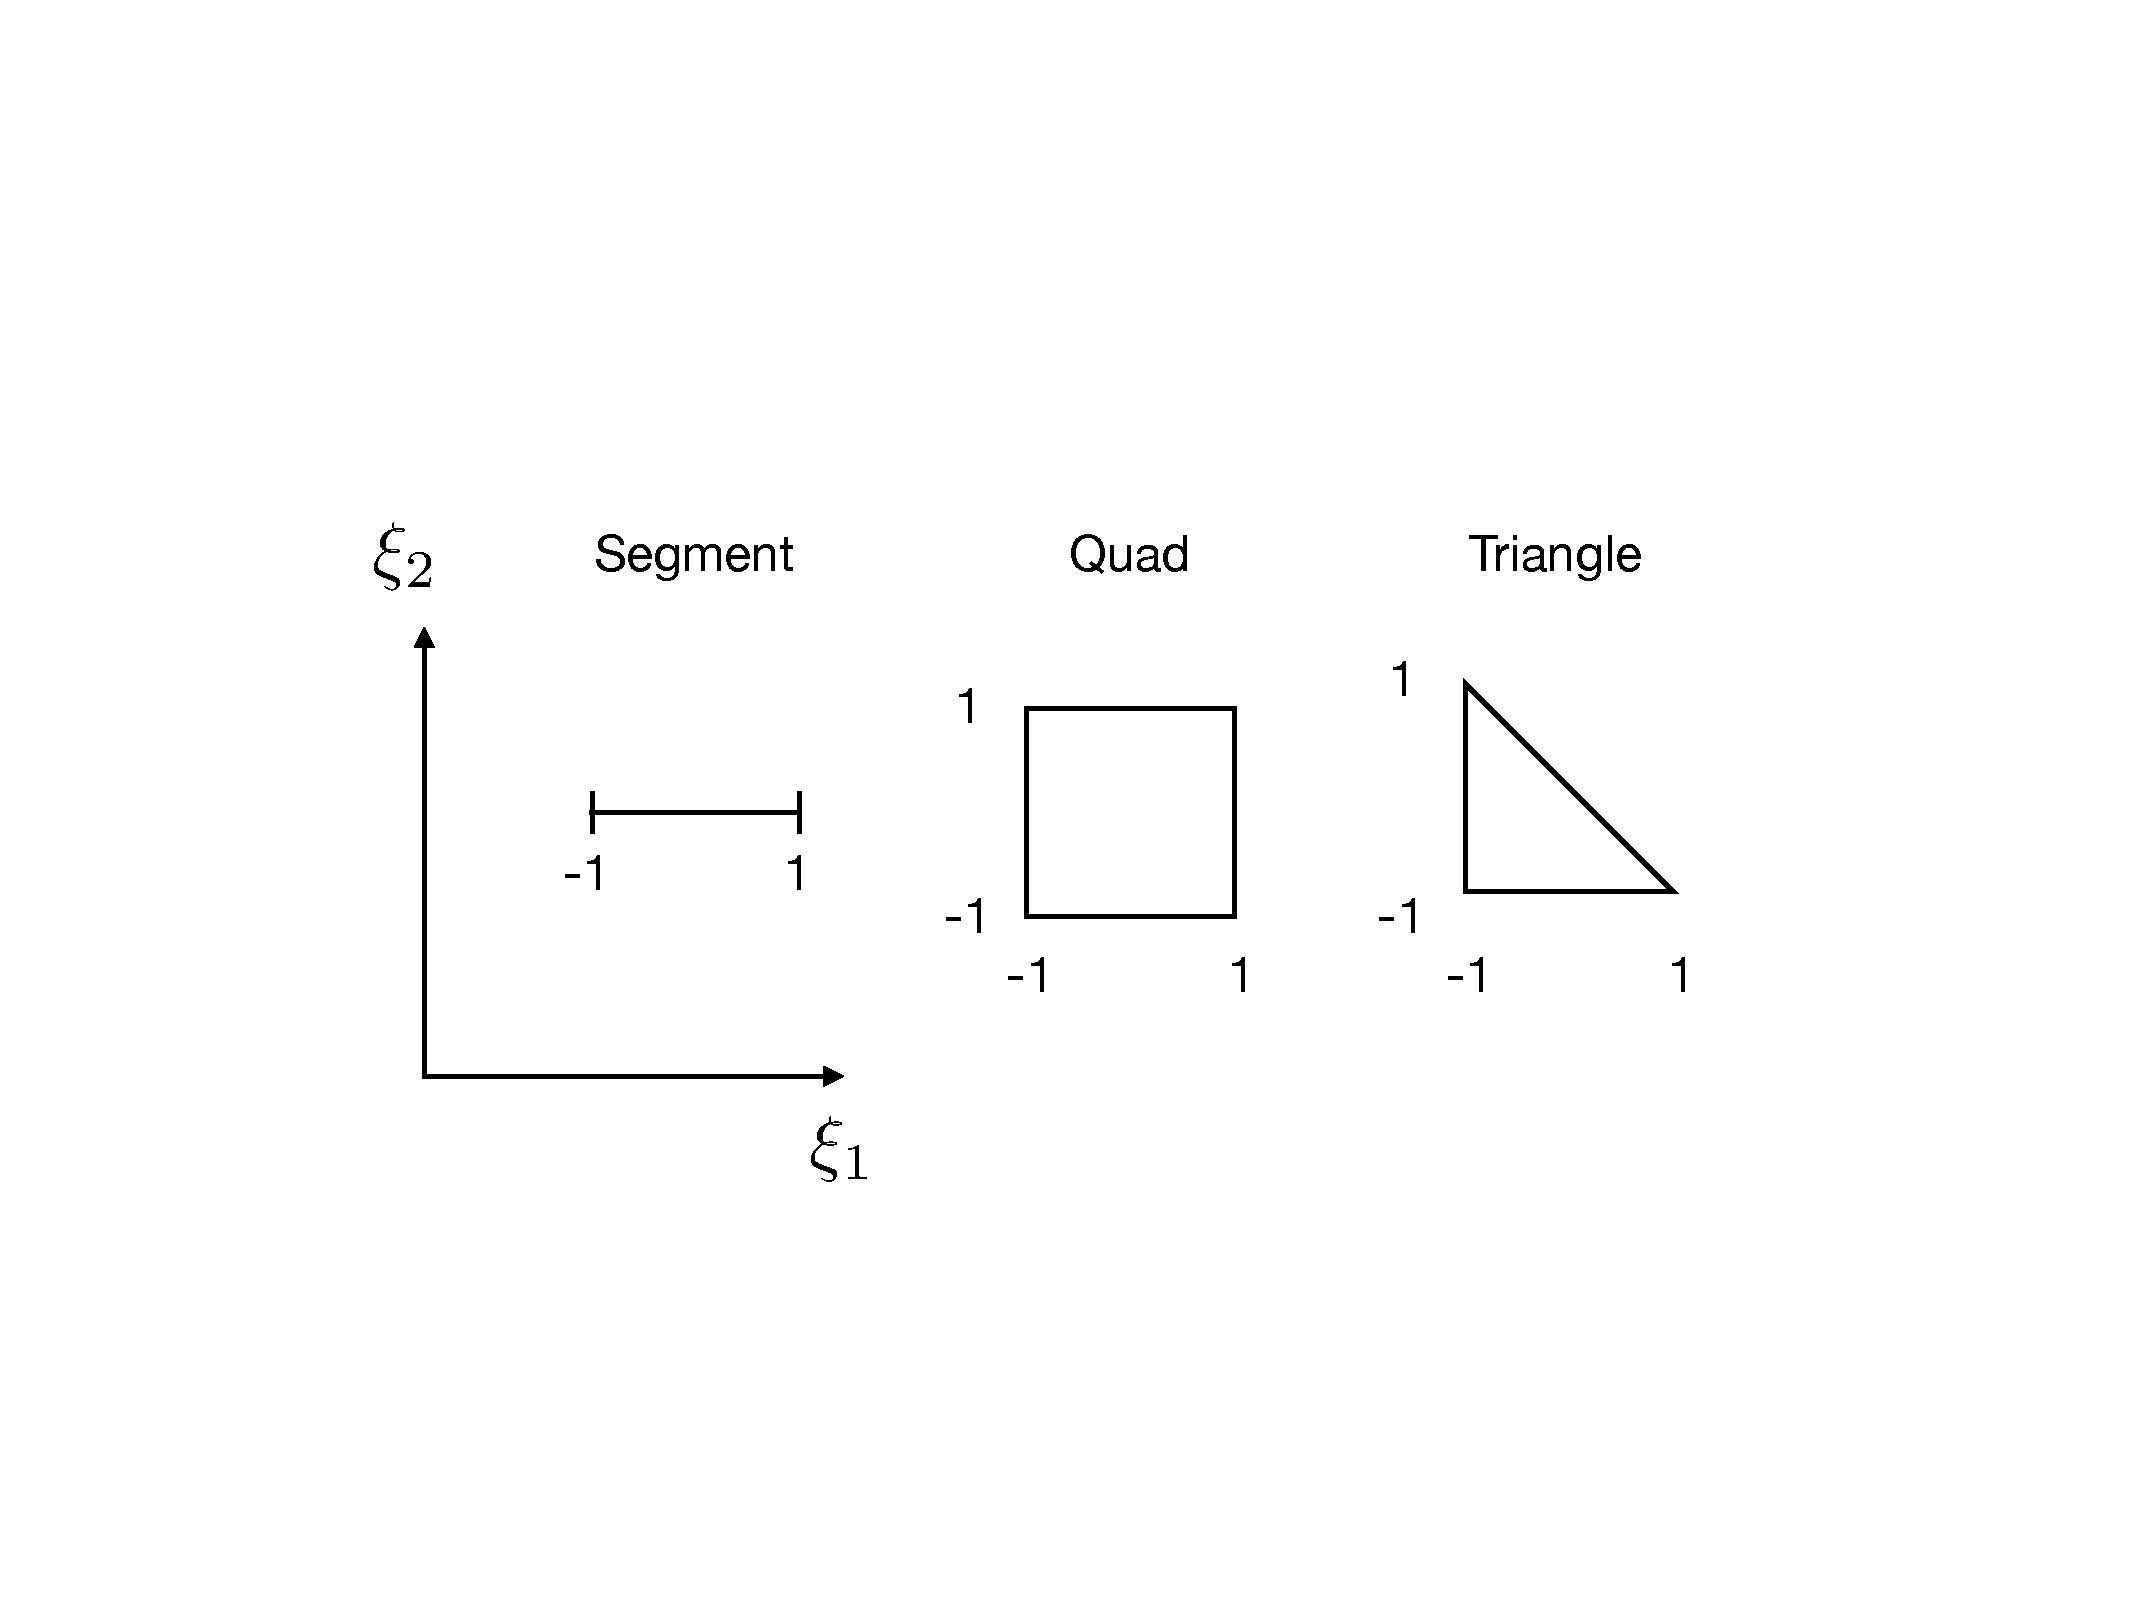
\includegraphics[width=4in]{img/refelement.pdf}
\caption{Example of the 1D and 2D reference space elements (segment, quad and triangle).}
\label{stdregions:refelement}
\end{figure}

The standard quad and standard hexahedra (shorthanded 'hex') are geometrically tensor-product constructions defined
on $[-1,1]^d$ for $d=2$ and $d=3$ respectively.  The standard triangle is constructed by taking $\xi_1 \in [-1,1]$ and taking $\xi_2 \le -\xi_1$.
The standard tetrahedra (shorthanded 'tet') is built upon the standard triangle and has all four faces being triangles, with the two
triangles along the coordinate directions looking like the standard triangle.  The standard prism consists of a standard 
triangle along the $\xi_1--\xi_2$ plane extruded into the third direction (yielding three quadrilateral faces).  The standard
pyramid consists of a standard quadrilateral at the base with four triangular faces reaching up to its top vertex  We show this
pictorially in Figure \ref{stdregions:3dshapes}.


\begin{figure}[htb]
\centering
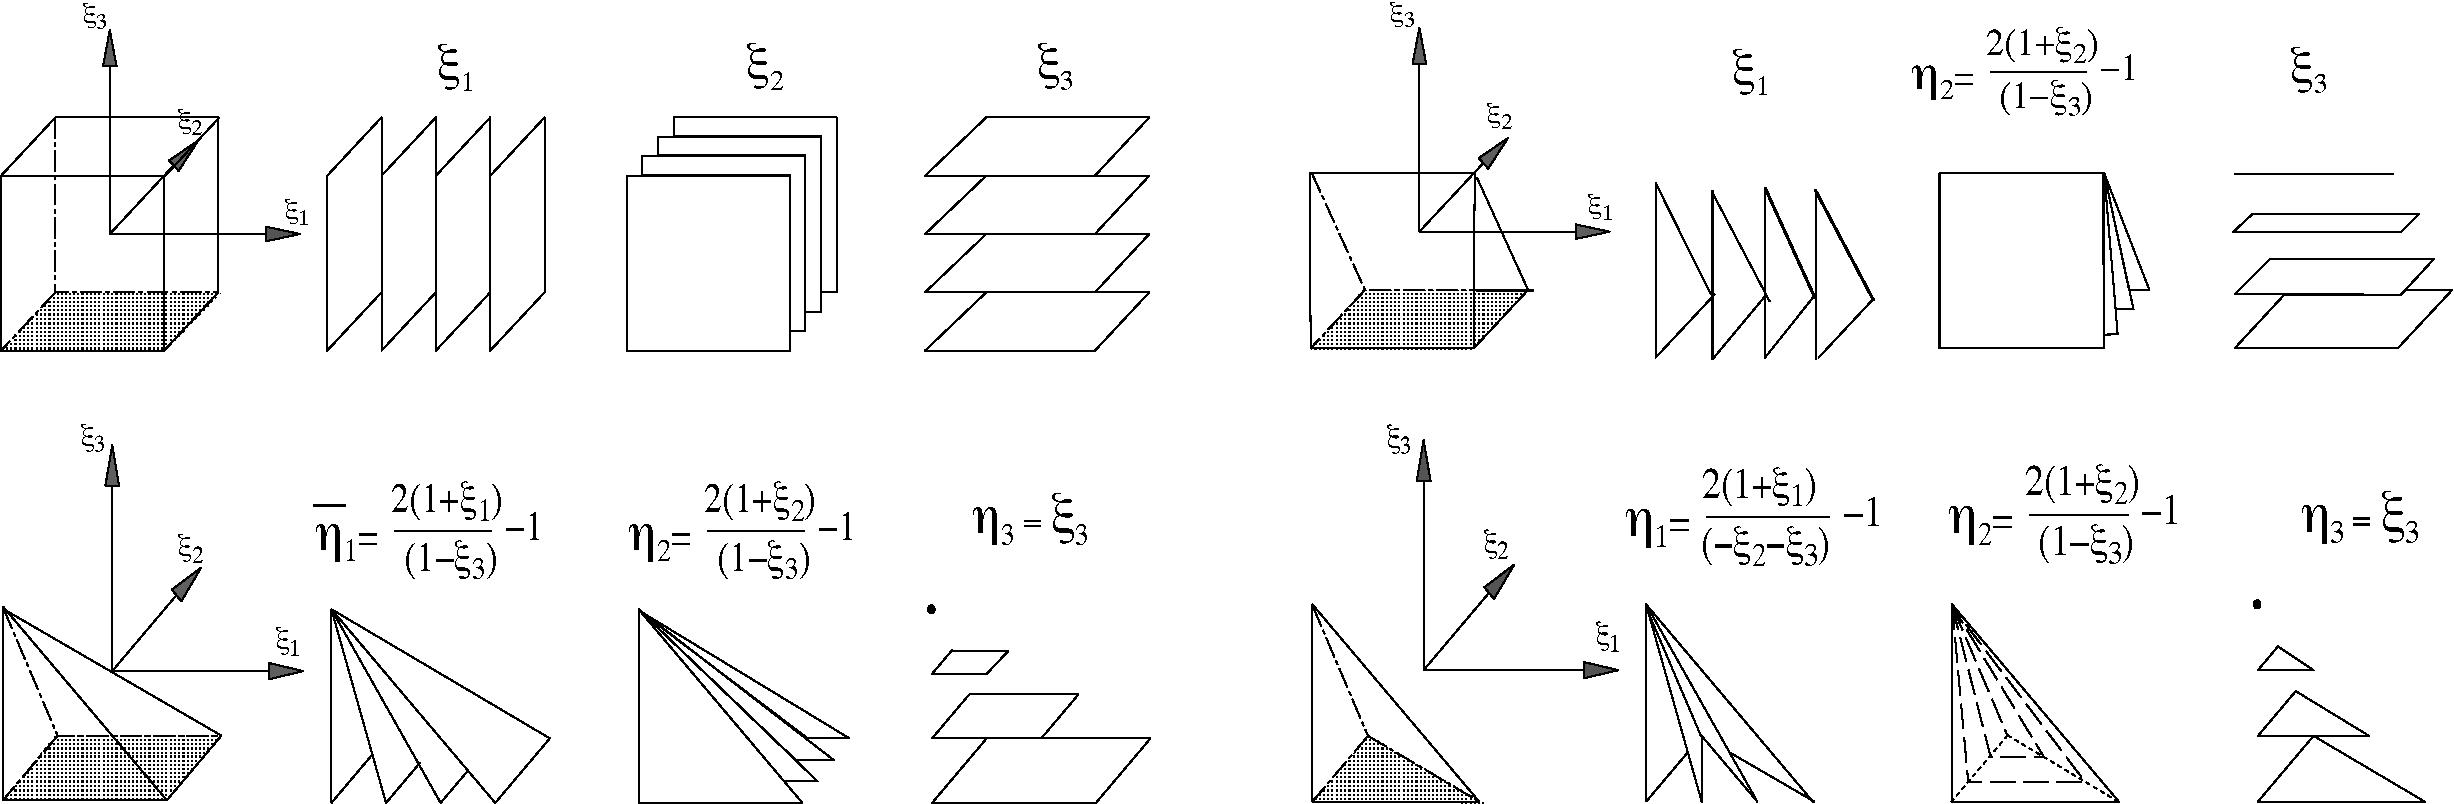
\includegraphics[width=4in]{img/LocalCoords.pdf}
\caption{Hexahedron to tetrahedron transformation showing how to go from an element on $[-1,1]^3$ (i.e. a standard hexahedron) to the three other element types which are subsets on $[-1,1]^3$.  Image taken from \cite{KaSh05}.}
\label{stdregions:3dshapes}
\end{figure}

Regardless of the particular element type, we use the fact one can build polynomial spaces over these geometric 
objects.  In the case of triangles and tetrahedra, these are polynomial spaces in the mathematical sense, i.e. $\mathcal{P}(k)$
spaces.  In the case of quadrilaterals and hexahedra, these are bi-- and tri-polynomial spaces, i.e. $\mathcal{Q}(k)$. 
In the case of prisms and pyramids, the spaces are more complicated and are a mixture in some sense of these spaces, but
they are indeed polynomial in form.  This allows us to define differentiation exactly and to approximate integrals
exactly up to machine precision.

In what is to follow, we describe (1) how you can build differentiation and integration operators over standard regions by mapping
them to a domain over which you can exploit index separability; and then (2) how you can build differentiation and integration operators
natively over various standard region shapes.  The former allows one to benefit from tensor-product operators, and is at present the 
primary focus of all {\nek} operators.  The latter as implemented for nodal element types is currently an {\em is-a} class definition 
extended from the (tensor-product-based) standard element definitions.



%%%%%%%%%%%%%%%%%%%%%%%%%%%%%%%%%%%%%%%%
\subsection{Reference Element Transformations That Facilitate Separability}

Differentiation and integration over the standard elements within {\nek}, in general, always try to map things back to tensor-product
(e.g. tensor-contraction indexing).  This allows one to transform operators that would normally have iterators that go from $i=0,\ldots,N^d$ 
where $d$ is the dimension of the shape to operators constructed with $d\cdot N$ operations (i.e., the product of one-dimensional operations).

As an example (to help the reader gain an intuitive understanding), consider the integration of a function $f(\vec{x})$ over a 
hexahedral element.  If we had a quadrature rule in 3D that needed $N^d$ points to integrate this function exactly, we would
express the operation as:

\begin{equation*}
\int_E f(\vec{x})\, d\vec{x} \approx \sum_{i=0}^{N^d} \omega_{i}\, f(\vec{z}_i)
\end{equation*}

\noindent where $E$ denotes our $d$-dimensional element and the set $Q = \{\vec{z}_i,\omega_i\}$ denotes the set of 
points and quadrature weights over the element $E$.  Now, suppose that both our function $f(\vec{x})$ and our $Q$ were
separable: that is, $f(\vec{x})$ can be written as $f_1(x_1)\cdot f_2(x_2)\cdot f_3(x_3)$ where $\vec{x} = (x_1,x_2,x_3)^T$
and $Q$ can we written in terms of 1D quadrature: $\vec{z}_i = z^{(1)}_{i_1}\cdot z^{(2)}_{i_2} \cdot z^{(3)}_{i_3}$ with
the index handled by an index map $\sigma$ defined by $i=\sigma(i_1,i_2,i_3)= i_1 + N\cdot i_2 + N^2 \cdot i_3$,
and similarly for the weights $\omega_i$.  We can then re-write the integral above as follows:

\begin{eqnarray*}
\int_E f(\vec{x})\, d\vec{x} &=& \int_E f(x_1)\cdot f(x_2) \cdot f(x_3)\,dx_1\,dx_2\,dx_3 \\
&\approx & \sum_{i=0}^{N^d} \omega_{i}\, f(\vec{z}_i) \\
&=& \sum_{i_1=0}^N \sum_{i_2=0}^N \sum_{i_3=0}^N \omega_{\sigma(i_1,i_2,i_3)}\, [f(z^{(1)}_{i_1})\cdot f(z^{(2)}_{i_2}) \cdot f(z^{(3)}_{i_3})] \\
&=& \left[ \sum_{i_1=0}^N \omega_{i_1}\,f(z^{(1)}_{i_1})\right]\cdot \left[ \sum_{i_2=0}^N \omega_{i_2}\,f(z^{(2)}_{i_2})\right] \cdot \left[ \sum_{i_3=0}^N \omega_{i_3}\,f(z^{(3)}_{i_3})\right]
\end{eqnarray*}

As you can see, when the functions are separable and the quadrature (or collocating points) can be written in separable form, we
can take $\mathcal{O}(N^d)$ operators and transform them into $\mathcal{O}(d\cdot N))$ operators.  The above discussion is
mainly focusing on the mathematical transformations needed to accomplish this; in subsequent sections, we will point out the 
memory layout and index ordering (i.e. now $\sigma$ is ordered and implemented) to gain maximum performance.

The discussion of tensor-product operations on quadrilaterals and hexahedra may seem quite natural as the element construction
is done with tensor-products of the segment; however, how do you create these types of operations on triangles (and anything
involving triangles such as tetrahedra, prisms and pyramids)?  The main mathematical building block we use that allows such
operators is a transformation due to Duffy \cite{Duffy82}, which was subsequently used by Dubiner \cite{Dubiner91} in the context
of finite elements  and was extended to general polyhedral types by Ainsworth \cite{AinsworthAD11,Ainsworth14}.

An image denoting the Duffy transformation is shown in Figure \ref{stdregions:duffy}.  On the left is an example of the
right-sided standard triangle with coordinate system $(\xi_1,\xi_2)$, and on the right is the separable tensor-product
domain with coordinates $(\eta_1,\eta_2)$.  We often refer to this transformation as ``collapsed coordinates" as it
appears as the ``collapsing" of a quadrilateral domain to a triangle.    Note that the edge along $\eta_1 = 1$ on
the quadrilateral collapses down to the single point $(\xi_1,\xi_2)=(1,1)$.  This, in general, does not cause issues
with our integration over volumes as this is a point of measure zero.  However, special case will need be taken when
doing edge integrals.  We will make it a point to highlight those places in which special care is needed.

\begin{figure}[htb]
\centering
\includegraphics[width=4in]{img/afg002.pdf}
\caption{Duffy mapping between a right-sided triangle and a square domain.}
\label{stdregions:duffy}
\end{figure}


With the 2D Duffy transformation in place, we can actually create all four 3D element types from the starting point
of a hexahedra (our base tensor-product shape).  One collapsing operation yields a prism.  The second collapsing
operation yields a pyramid.  Lastly, a final collapsing operation yields a tetrahedra.  A visual representation of these
operations are shown in Figure \ref{stdregions:3Dduffy}.

\begin{figure}[htb]
\centering
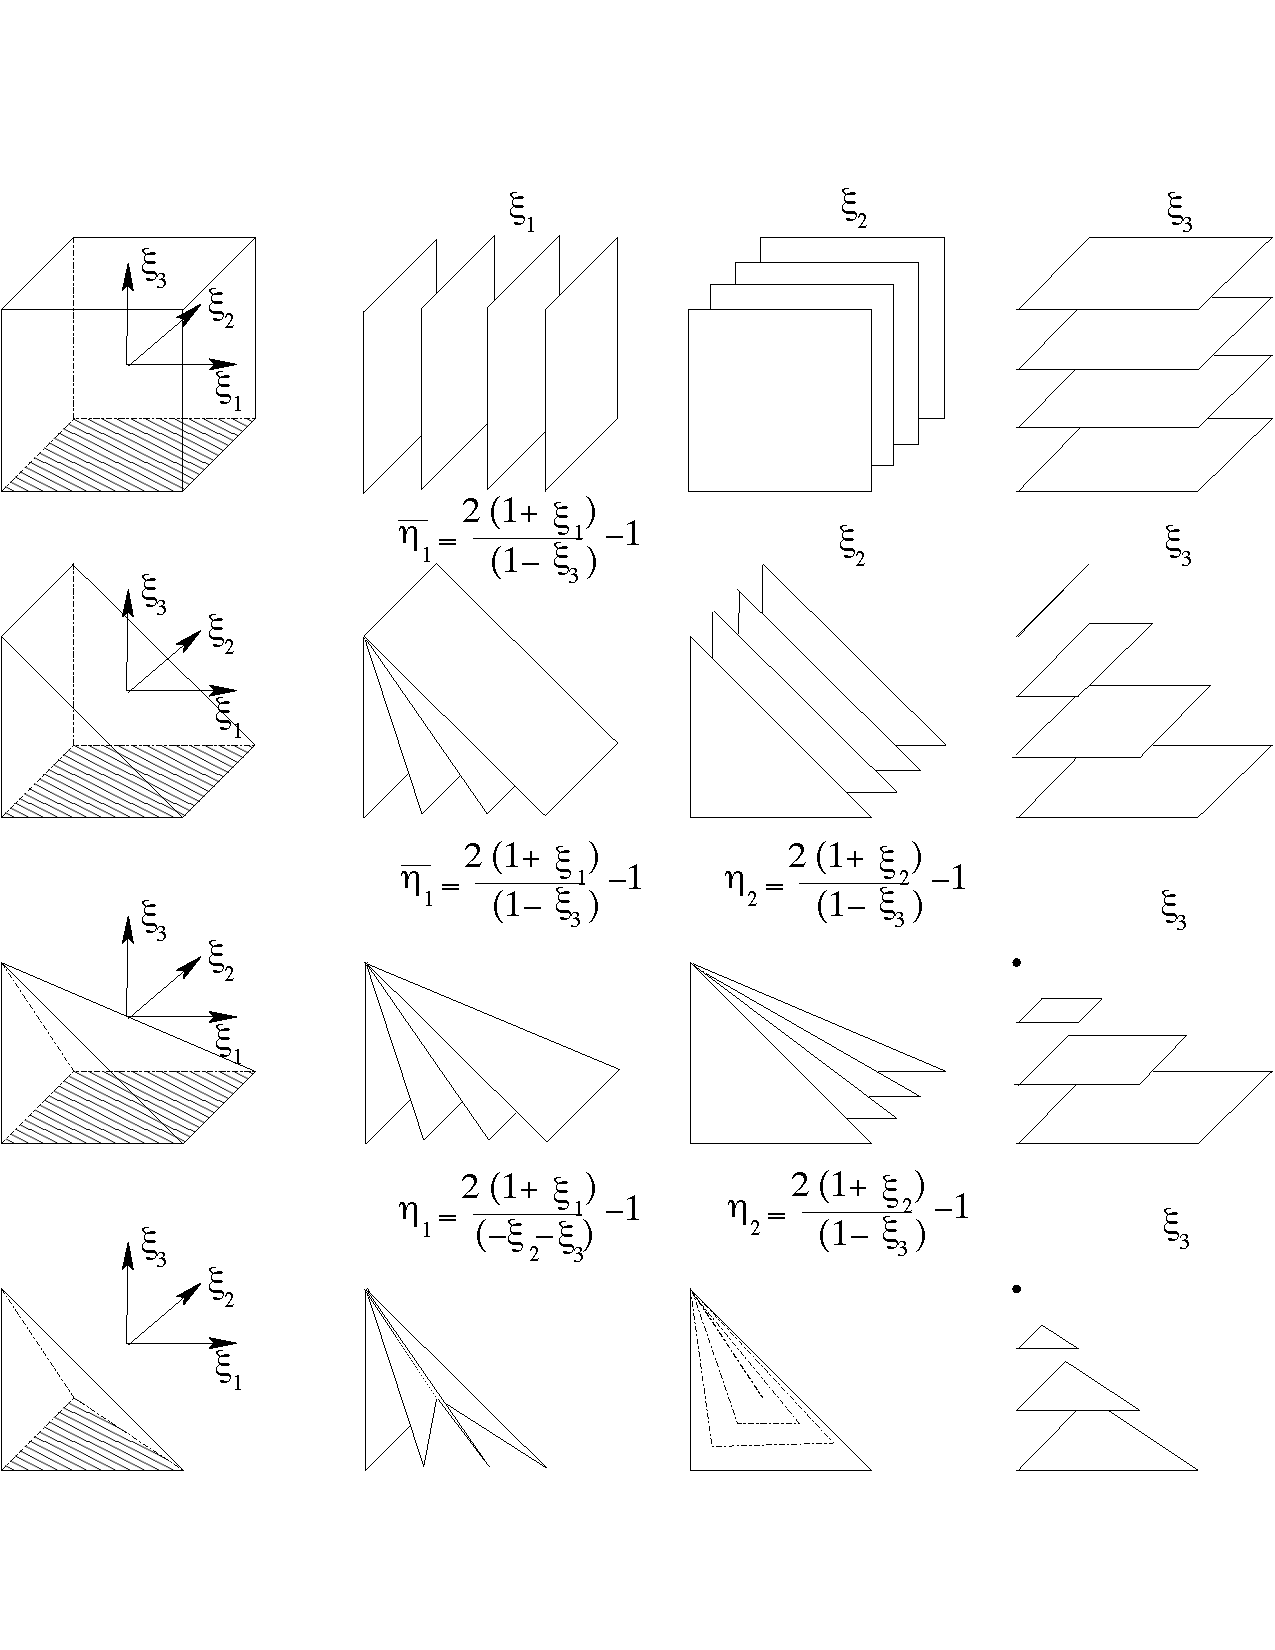
\includegraphics[width=4in]{img/3dcoords.pdf}
\caption{Duffy mapping application to generate all the 3D element types.  Image taken from \cite{KaSh05}.}
\label{stdregions:3Dduffy}
\end{figure}

This is meant merely to be a summary of tensor-product operations, enough to allow us to discuss the basic
data types and algorithms within {\nek}.  If more details are needed, we encourage the reader to consult
Karniadakis and Sherwin \cite{KaSh05} and the references therein.

%%%%%%%%%%%%%%%%%%%%%%%%%%%%%%%%%%%%%%%%
\subsection{Reference Elements On Primitive Geometric Types}

Although the primary backbone of {\nek} is tensor-product operations across all element types through the 
use of collapsed coordinates, we have implemented two commonly used non-tensorial basis set definitions.  
These are based upon Lagrange polynomial construction from a nodal (collocating) point set.  As derived
element types (in the $C++$ sense), we have implemented NodalStdTriangle (and Tet) based upon
the electrostatic points of Hesthaven \cite{Hesthaven98} and the Fekete points of 
Taylor and Wingate \cite{TaylorW99,TaylorWV00}.

Although these types of elements, at first glance, might seem to be ``sub-optimal" (in terms of operations), there
are various reasons why people might choice to use them.  For instance, the point set you use for defining 
the collocation points dictates the interpolative projection operator (and correspondingly the properties of that
operator) -- an important issue when evaluating boundary conditions, initial conditions and for some non-linear operator
evaluations.  Within the {\nek} team, we started an examination of this within the paper by 
Kirby and Sherwin \cite{KirbyS06}.  There has since been various papers in the literature (beyond the scope of this
developer's guide) that give the pros and cons of tensor-product (separable) and non-tensor-product element
types.  


%
%
\section{The Fundamental Data Structures within StdRegions}
\label{sec:stdregions-datastructures}

In almost all object-oriented languages (which includes $C++$), there exists the concepts of {\em class attributes} and {\em object attributes}.  Class attributes are those attributes shared by all object instances (both immediate and derived objects) of a particular class definition, and object attributes (sometimes called data members) are those attributes whose values vary from object to object and hence help to characterize (or make unique) a particular object. In $C++$, object attributes are specified a header file containing class declarations; within a class declaration, attributes are grouped by their accessibility: {\em public} attributes, {\em protected} attributes and {\em private} attributes.  A detailed discussion of the nuances of these
categories are beyond the scope of this guide; we refer the interested reader to the following books for further details:  \cite{BStroustrup,SMeyers}.
For our purposes, the main thing to appreciate is that categories dictate access patters within the inheritance hierarchy and to the ``outside'' world 
(i.e. access from outside the object).  We have summarized the relationships between the categories and their accessibility in Tables
\ref{table:stdreg_publicinheritance}, \ref{table:stdreg_protectedinheritance} and \ref{table:stdreg_privateinheritance} \footnote{These tables are based upon information provided at http://www.programiz.com/cpp-programming/public-protected-private-inheritance, accessed 6 April 2018.}.


\begin{table}[ht]
\begin{center}
\caption{Accessibility in Public Inheritance}
\begin{tabular}{c c c c}
\hline\hline
Accessibility & private variables & protected variables & public variables \\
\hline
Accessibility from own class? & yes & yes & yes \\
Accessibility from derived class? & no & yes & yes\\
Accessibility from 2nd derived class? & no & yes & yes\\
\end{tabular}
\end{center}
\label{table:stdreg_publicinheritance}
\end{table}

\begin{table}[ht]
\begin{center}
\caption{Accessibility in Protected Inheritance}
\begin{tabular}{c c c c}
\hline\hline
Accessibility & private variables & protected variables & public variables \\
\hline
Accessibility from own class? & yes & yes & yes \\
Accessibility from derived class? & no & yes & yes \\
&&&(inherited as \\
&&&protected variable)\\
Accessibility from 2nd derived class? & no & yes & yes\\
\end{tabular}
\end{center}
\label{table:stdreg_protectedinheritance}
\end{table}

\begin{table}[ht]
\begin{center}
\caption{Accessibility in Private Inheritance}
\begin{tabular}{c c c c}
\hline\hline
Accessibility & private variables & protected variables & public variables \\
\hline
Accessibility from own class? & yes & yes & yes\\
Accessibility from derived class? & no & yes & yes \\
& & (inherited as & (inherited as \\
& & private variable) &  private variable) \\
Accessibility from 2nd derived class? & no & no & no \\
\end{tabular}
\end{center}
\label{table:stdreg_privateinheritance}
\end{table}

Within the StdRegions directory of the library, there exists a class inheritance hierarchy designed to try to encourage re-use of core
algorithms (while simultaneously trying to minimize duplication of code).  We present this class hierarchy in Figure \ref{stdregions:stdexpansiontree}.

\begin{figure}[htb]
\centering
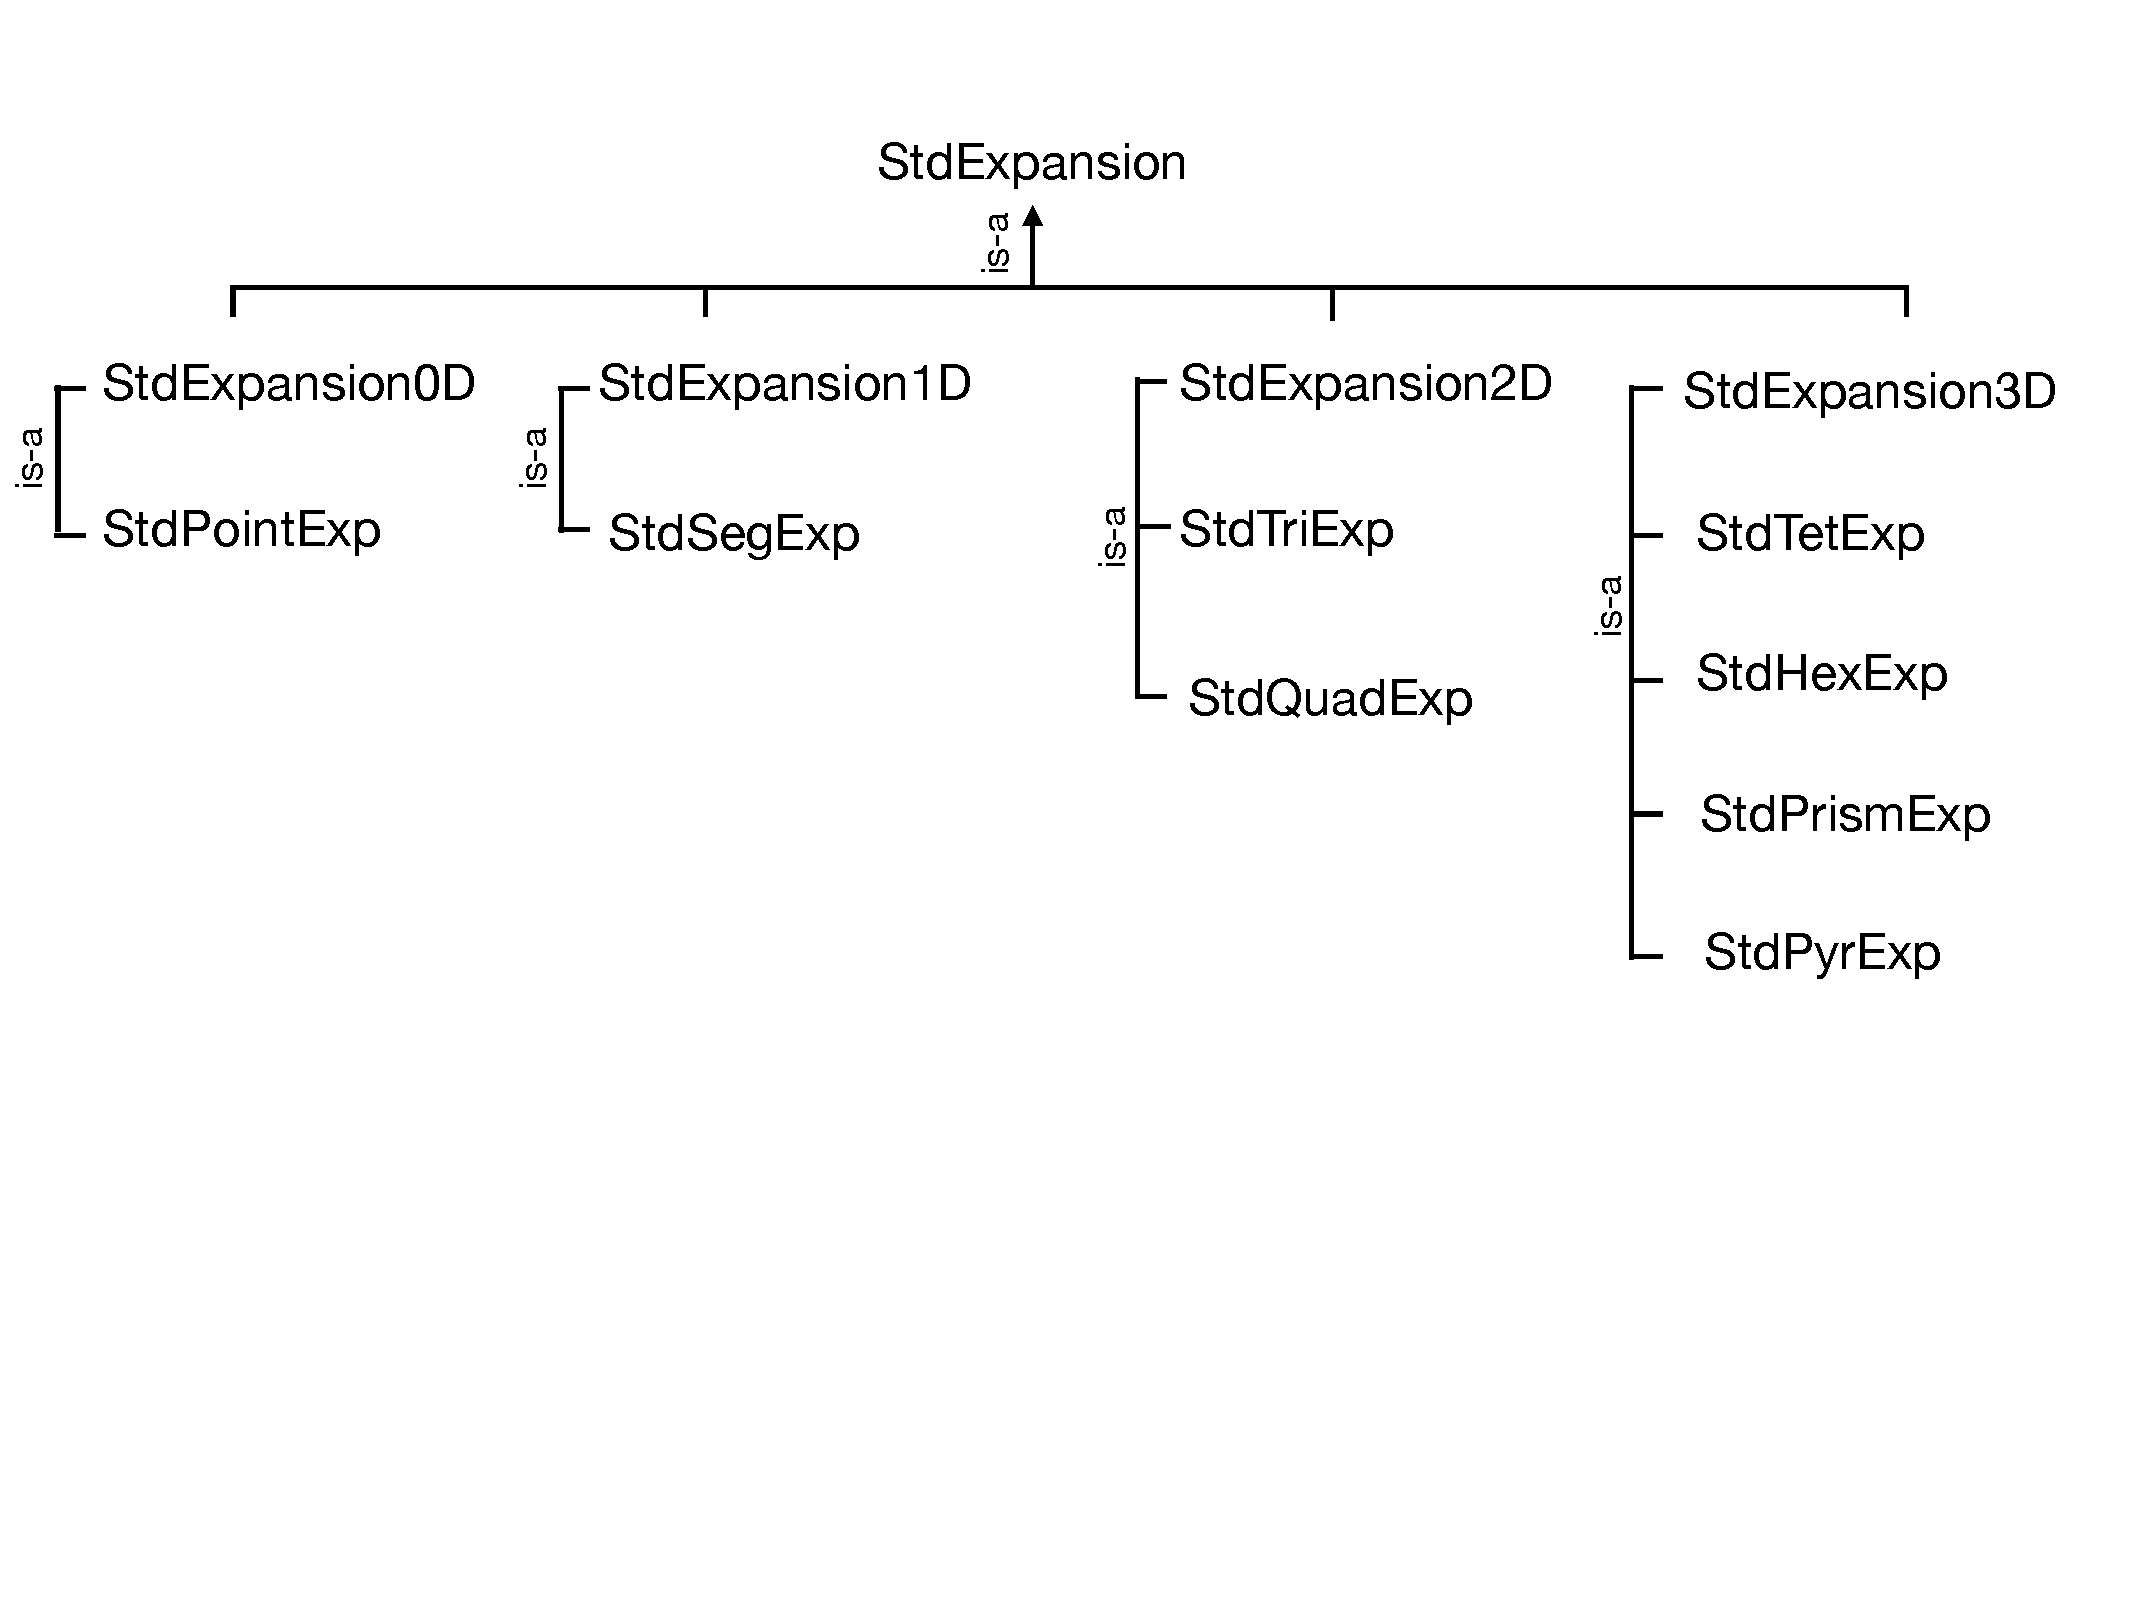
\includegraphics[width=6in]{img/stdexpansiontree.pdf}
\caption{Class hierarchy derived from StdExpansion, the base class of the StdRegions Directory.}
\label{stdregions:stdexpansiontree}
\end{figure}

As is seen in Figure \ref{stdregions:stdexpansiontree}, the StdRegions hierarchy consists of three levels:  the base level from which all
StdRegion objects are derived is StdExpansion.   This object is then specialized by dimension, yielding StdExpansion0D, 
StdExpansion1D, StdExpansion2D and StdExpansion3D.  The dimension-specific objects are then specialized based upon
shape.  

The object attributes (variables) at various levels of the hierarchy can be understood in light of Figure \ref{stdregions:stdexpansion}.
At its core, an expansion is a means of representing a function over a canonically-defined region of space evaluated at a collection of point positions.
The various data members hold information to allow all these basic building blocks to be specified.

\begin{figure}[htb]
\centering
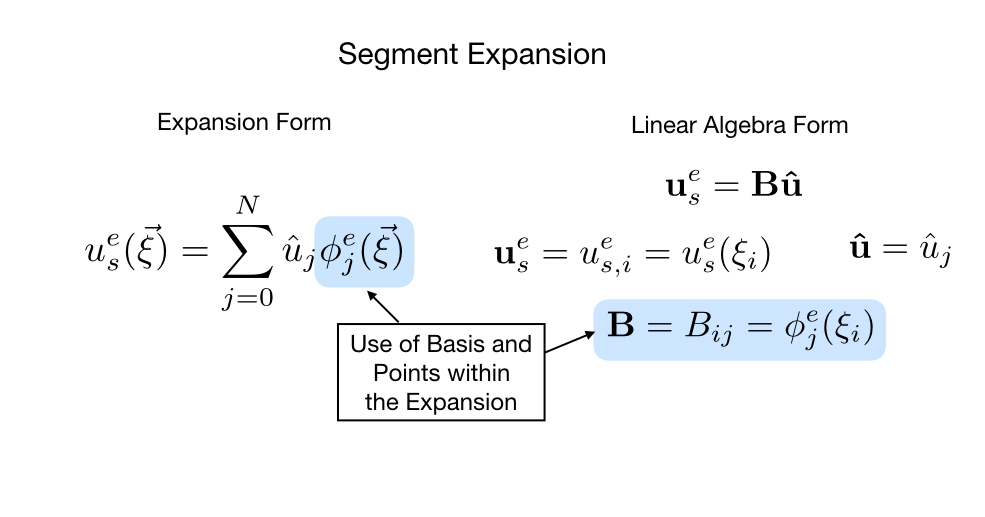
\includegraphics[width=6in]{img/StdExpansion.png}
\caption{Diagram to help understand the various data members (object attributes) contained within StdRegions and how they connect with the mathematical representation presented earlier.}
\label{stdregions:stdexpansion}
\end{figure}

The various private, protected and public data members contained within StdRegions are provided in the subsequent sections.

%%%%%%%%%%%%%%%%%%%%%%%%%%%%%%%%%%%%%%%%
\subsection{Variables at the Level of StdExpansion}

\paragraph{Private:}

There are private methods but no private data members within StdExpansion.

\paragraph{Protected:}

\begin{itemize}
\item  Array of Basis Shared Pointers:  \verb+m_base+
% 
\item  Integer element id: \verb+m_elmt_id+
%
\item Integer total number of coefficients in the expansion:  \verb+m_ncoeffs+
%
\item Matrix Manager: \verb+m_stdMatrixManager+
%
\item Matrix Manager: \verb+m_stdStaticCondMatrixManager+
%
\item IndexKeyMap Matrix Manager: \verb+m_IndexMapManager+
\end{itemize}


\paragraph{Public:}

There are public methods but no public data members within StdExpansion.



%%%%%%%%%%%%%%%%%%%%%%%%%%%%%%%%%%%%%%%%
\subsection{Variables at the Level of StdExpansion\$D for various Dimensions}

\paragraph{Private:}

There are private methods but no private data members within StdExpansion\$D.

\paragraph{Protected:}


\begin{itemize}
\item 0D and 1D: std::map<int, NormalVector> \verb+m_vertexNormals+
%
\item 2D: Currently does not have any data structure.  It should probably have \verb+m_edgeNormals+
%
\item 3D: std::map<int, NormalVector> \verb+m_faceNormals+
%
\item 3D: std::map<int, bool> \verb+m_negatedNormals+
\end{itemize}

\paragraph{Public:}

There are public methods but no public data members within StdExpansion\$D.

%%%%%%%%%%%%%%%%%%%%%%%%%%%%%%%%%%%%%%%%
\subsection{Variables at the Level of Shape-Specific StdExpansions}

\paragraph{Private:}

\paragraph{Protected:}

\paragraph{Public:}


%%%%%%%%%%%%%%%%%%%%%%%%%%%%%%%%%%%%%%%%
\subsection{General Layout of the Basis Functions in Memory}

\subsection{General Layout}

Basis functions are stored in a 1D array indexed by both mode and quadrature point. The fast index runs over quadrature points while the slow index runs over modes. This was done to match the memory access pattern of the inner product, which is the most frequently computed kernel for most solvers.

Bases are built from the tensor product of three different equation types (subsequently called Type 1, Type II and Type III respectively):
\begin{equation}
    \phi_{p}(z) =
    \begin{cases}
        \frac{1 - z}{2} & p = 0 \\
        \frac{1 + z}{2} & p = 1 \\
        \left(\frac{1-z}{2}\right)\left(\frac{1+z}{2}\right) P_{p-1}^{1,1}(z) & 2 \leq p < P
    \end{cases}
\end{equation}

\[
    \phi_{pq}(z) = \left\{
    \begin{array}{lll}
        \phi_{q}(z) & p = 0 & 0 \leq q < P \\
        \left(\frac{1 - z}{2}\right)^p & 1 \leq p < P & q = 0 \\
        \left(\frac{1-z}{2}\right)^p \left(\frac{1+z}{2}\right) P_{q-1}^{2p-1,1}(z) & 1 \leq p < P, & 1 \leq q < P - p
    \end{array}\right.
\]

\[
    \phi_{pqr}(z) = \left\{
    \begin{array}{llll}
        \phi_{qr} & p = 0 & 0 \leq q < P & 0 < r < P - q \\
        \left(\frac{1-z}{2}\right)^{p+q} & 1 \leq p < P, & 0 \leq q < P - p, & r = 0 \\
        \left(\frac{1 - z}{2}\right)^{p + q} \left(\frac{1+z}{2}\right) P_{r-1}^{2p + 2q - 1, r}(z) & 1 \leq p < P, & 0 \leq q < P - p, & 1 \leq r < P - p - qr.
    \end{array}\right.
\]

Here, $P$ is the polynomial order of the basis and $P^{\alpha,\beta}_{p}$ are the $p^{\text{th}}$ order jacobi polynomial.

\subsubsection{A Note Concerning Adjustments For $C_0$ Continuity}


Before going further it is worth reviewing the spatial shape of each node. The term $\frac{1 + z}{2}$ is an increasing function which is equal to zero at $z = -1$ and equal to one at $z = 1$. Similarly, $\frac{1 - z}{2}$ is a decreasing function which is equal to one at $z = -1$ and equal to zero at $z = +1$. These two functions are thus non-zero at one of each of the boundaries. If we need to maintain $C_0$ continuity with surrounding elements (as we do in the continuous Galerkin method), then these local modes must be assembled together with the correct local modes in adjacent elements to create a continuous, global mode. For instance $\frac{1 + z}{2}$ in the left element would be continuous with $\frac{1 - z}{2}$ in the right element. The union of these two modes under assembly form a single ``hat'' function. By contrast, functions of the form
\[
    \frac{1 - z}{2} \frac{1 + z}{2}
\]
are zero at both end points $z = \pm 1$. As a result, they are trivially continuous with any other function which is also equal to zero on the boundary. These ``bubble'' functions may be treated entirely locally and thus are used to construct the interior modes of a basis. Only bases with $p > 1$ have interior modes.

All of this holds separately in one dimension. Higher dimensional bases are constructed via the tensor product of 1D basis functions. As a result, we end up with a greater number of possibilities in terms of continuity. When the tensor product is taken between two bubble functions from different bases, the result is still a bubble function. When the tensor product is taken between a hat function and a bubble function we get ``edge'' modes (in both 2D and 3D). These are non-zero along one edge of the standard domain and zero along the remaining edges. When the tensor product is taken between two hat functions, they form a ``vertex'' mode which reaches its maximum at one of the vertices and is non-zero on two edges.  The 3D bases are constructed similarly.

Based upon this convention, the 1D basis set consists of vertex modes and bubble modes.  The 2D basis function set consists of vertex modes, edge modes and bubble modes.  The 3D basis set contains vertex modes, edge modes, face modes and bubble modes.

\subsection{2D Geometries}

\subsubsection{Quadrilateral Element Memory Organization}
Quads have the simplest memory organization. The quadrilateral basis is composed of the tensor product of two Type I functions $\phi_p(\xi_{0,i}) \phi_q(\xi_{1,j})$. This function would then be indexed as

\begin{lstlisting}
    basis0[p*nq0 + i] * basis1[q*nq1 + j]
\end{lstlisting}
where nq<b> is the number of quadrature points for the $b^{\text{th}}$ basis. Unlike certain mode orderings (e.g. Karniadakis and Sherwin \cite{KaSh05}), the two hat functions are accessed as the first and second modes in memory with interior modes placed afterward. Thus,
\begin{lstlisting}
    basis[i], basis[nq + i]
\end{lstlisting}
correspond to $\frac{1 - z}{2}$ and $\frac{1 + z}{2}$ respectively.

\subsubsection{Triangle Element Memory Organization}
Due to the use of collapsed coordinates, triangular element bases are formed via the tensor product of one basis function of Type I, and one of Type II, i.e. $\phi_p(\eta_{0,i} \phi_pq(\eta{1,j}))$. Since $\phi_p$ is also a Type I function, its memory ordering is identical to that used for quads. The second function is complicated by the mixing of $\xi_0$ and $\xi_1$ in the construction of $\eta_1$.

In particular, this means that the basis function has two modal indices, $p$ and $q$. While $p$ can run all the way to $P$, The number of $q$ modes depends on the value of the $p$ index q index such that $0 \leq q < P - p$. Thus, for $p = 0$, the q index can run all the way up to $P$. When p = 1, it runs up to $P - 1$ and so on. Memory is laid out in the same way starting with $p=0$. To access all values in order, we write
\begin{lstlisting}
    mode = 0
    for p in P:
        for q in P - p:
            out[mode*nq + q] = basis0[p*nq]*basis1[mode*nq + q]
        mode += P-p
\end{lstlisting}
Notice the use of the extra ``mode'' variable. Since the maximum value of $q$ changes with $p$, basis1 is not simply a linearized matrix and instead has a triangular structure which necessitates keeping track of our current memory location.

The collapsed coordinate system introduces one extra subtlety. The mode
\[
    \phi_1(\eta_1) \phi_1(\eta_2)
\]
represents the top right vertex in the standard basis. However, when we move to the standard element basis, we are dealing with a triangle which only has three vertices. During the transformation, the top right vertex collapses into the top left vertex. If we naively construct an operators by iterating through all of our modes, the contribution from this vertex to mode $\Phi_{01}$ will not be included. To deal with this, we add its contribution as a correction when computing a kernel. The correction is $\Phi_{01} = \phi_0 \phi_{01} + \phi_1 \phi_{10}$ for a triangle.

\subsection{3D Geometries}

\subsubsection{Hexahedral Element Memory Organization}
The hexahedral element does not differ much from the quadrilateral as it is the simply the product of three Type I functions.
\[
    \Phi_{pqr} = \phi_p(\xi_0) \phi_q(\xi_1) \phi_r(\xi_2).
\]

\subsubsection{Prismatic Element Memory Organization}
Cross sections of a triangular prism yield either a quad or a triangle based chosen direction. The basis, therefore, looks like a combination of the two different 2D geometries.
\[
    \Phi_{pqr} = \phi_p(\eta_0)\phi_q(\xi_1)\phi_{pr}(\eta_1).
\]
Taking $\phi_p \phi_{pr}$ on its own produces a triangular face while taking $\phi_p \phi_q$ on its own produces a quadrilateral face. When the three basis functions are combined into a single array (as in the inner product kernel), modes are accessed in the order p,q,r with r being the fastest index and p the slowest. The access pattern for the prism thus looks like
\begin{lstlisting}
    mode_pqr = 0
    mode_pr = 0
    for p in P:
        for q in Q:
            for r in P - p:
                out[mode_pqr*nq + r] = basis0[p*nq]*basis1[q*nq]*basis2[mode_pr + r]
            mode_pqr += P - p
        mode_pr += P - p
\end{lstlisting}

As with the triangle, we have to deal with complications due to collapsed coordinates. This time, the singular vertex from the triangle occurs along an entire edge of the prism. Our correction must be added to a collection of modes indexed by $q$
\[
    \Phi_{0q1} += \phi_1 \phi_q \phi_{10}.
\]

\subsubsection{Tetrahedral Element Memory Organization}
The tetrahedral element is the most complicated of the element constructions. It cannot simply be formed as the composition of multiple triangles since $\eta_2$ is constructed by mixing three coordinate directions. We thus need to introduce our first Type III function.
\[
    \Phi_{pqr}(\eta_0, \eta_1, \eta_2) = \phi_{p}(\eta_0) \phi_{pq} (\eta_1) \phi_{pqr}(\eta_2).
\]
The $r$ index is constrained by both $p$ and $q$ indices. It runs from $P - p - q$ to $1$ in a similar manner to the Type II function. Our typical access pattern is thus
\begin{lstlisting}
mode_pqr = 0
mode_pq = 0
for p in P:
    for q in P - p:
        for r in P - p - r:
            out[mode_pqr*nq + r] = basis0[p*nq]*basis1[mode_pq + q]*basis2[mode_pqr + r]
        mode_pqr += (P - p - r)
    mode_pq += (P - p)
\end{lstlisting}
The tetrahedral element also has to add a correction due to collapsed coordinates. Similar to the prism, the correction must be applied to an entire edge indexed by $r$
\[
    \Phi_{01r} += \phi_1 \phi_1 \phi_{11r}.
\]

\subsubsection{Pyramidic Element Memory Organization}
Like the tetrahedral element, a pyramid contains a collapsed coordinate direction which mixes three standard coordinates from the standard region. Unlike the tetrahedra, the collapse only occurs along one axis. Thus it is constructed from two Type I functions and one Type III function
\[
    \Phi_{pqr} = \phi_p(\eta_1) \phi_q(\eta_2) \phi_{pqr}(\eta_3).
\]
The product $\phi_p \phi_q$ looks like the a quad construction which reflects the quad which serves as the base of the pyramid. A typical memory access looks like
\begin{lstlisting}
mode_pqr = 0
for p in P:
    for q in P - p:
        for r in P - p - r:
            out[mode_pqr*nq + r] = basis0[p*nq]*basis1[q*nq]*basis2[mode_pqr*nq + r]
        mode_pqr += (P - p - r)
\end{lstlisting}



%
%
\section{The Fundamental Algorithms within StdRegions}

As stated in the introduction, this section of this guide is structured in question-answer form.  This is not meant to capture every possible
question asked of us on the {\nek} users list; however, this set of (ever-growing) questions are meant to capture the ``big ideas'' that developers 
want to know about how StdRegions work and how they can be used.  

In this section, we will through question and answer format try to cover the following basic algorithmic concepts that are found within 
the StdRegions part of the library:

\begin{itemize}
\item xx
\end{itemize}

With the big ideas in place, let us now start into our questions.

\paragraph{Question:}


%%%%%%%%%%%%%%%%%%%%%%%%%%%%%%%
\chapter{Inside the Library: SpatialDomains}
\label{chap:spatialdomains}


In this chapter, we walk the reader through the different components
of the SpatialDomains Directory.  We begin with a discussion of the
mathematical fundamentals, for which we use the book by Karniadakis
and Sherwin \cite{KaSh05} as our principle reference.  We then provide
the reader with an overview of the primary data structures introduced
within the SpatialDomains Directory (often done through C++ objects),
and then present the major algorithms -- expressed as either object
methods or functions -- employed over these data structures.


The SpatialDomains Directory and its corresponding class definitions serve two principal purposes:
\begin{enumerate}
\item To hold the elemental geometric information (i.e. vertex information, curve information and reference-to-world mapping information); and
\item To facility reading in and writing out geometry-related information.
\end{enumerate}

When designing Nektar++, developing a class hierarchy for StdRegions
(those fundamental domains over which we define integration and
differentiation) and LocalRegions (i.e. elements in world-space) was
fairly straightforward following \cite{KaSh05}.  For instance, a
triangle in world-space {\em is-a} standard triangle.  The first
question that arose was where to store geometric information, as
information within the LocalRegions element or as information
encapsulated from the element so that multiple Expansions could all
point to the same geometric information.  The decision we made was to
store geometric information -- that is, the vertex information in
world-space that defines an element and the edge and face curvature
information -- in its own data structure that could be shared by
multiple Expansions (functions) over the same domain (element) in
world-space.  Hence SpatialDomains started as the directory containing
Geometry and GeomFactors class definitions to meet the first item
listed above.  A LocalRegion {\em is-a} StdRegion and {\em has-a}
SpatialDomain (i.e. Geometry and GeomFactors).

We then realized that in order to jump-start the process of
constructing elements and combining them together into MultiRegions
(collections of elements that represent a (sub)-domain of interest),
we needed devise a light-weight data structure into which we could
load geometric information from our geometry file and from which we
could then construct Expansions (with their mappings, etc.).  The
light-weight data structure we devised was MeshGraph, and it was meant
to meet the second item listed above.


%
\section{The Fundamentals Behind SpatialDomains}
\label{sec:spatialdomains-fundamentals}

As mentioned in our discussions of the fundamentals of StdRegions (i.e. Section \ref{sec:stdregions-fundamentals}), one of the most
fundamental tools from calculus that we regularly employ is the idea of mapping from general domains to canonical domains.  General
domains are the regions in world space over which we want to solve engineering problems, and thus want to be able to take derivatives and
compute integrals.  But as we learned in calculus, it is often non-trivial to accomplish differentiation or integration over these regions.  We resort
to the mapping arbitrary domains back to canonical domains over which we can define various operations.  We introduced our canonical domains,
which we call standard regions, in Chapter \ref{chap:stdregions}.  We refer to our world space regions as local regions, which we will present
in Chapter \ref{chap:localregions}.  How these two are connected are via SpatialDomains.  

As will be further discussed in Section \ref{sec:spatialdomains-datastructures}, there are two fundamental purposes served by SpatialDomains:  (1) holding
basic geometric information (e.g. vertex values and curvature information) and (2) holding geometric factors information.  The former information relates to 
the geometric way we map standard regions to local regions.  The latter information relates to how we use this map to allow us to accomplish 
differentiation and integration of functions in world space via operations on standard regions with associated map (geometric) information.  In this section,
we will highlight the important mathematical principles that are relevant to this section. We will first discuss the mapping itself:  vertex and curvature information
and how it is used.  We will then discuss how geometric factor information is computed.  We break this down into two subsections following the convention of the
code.  We will first discussed what is labeled in the code as {\em Regular}, and denotes mappings between elements of the same dimension 
(i.e. standard region triangles to 2D triangles in world space).  Although our notation will be slightly different, we will use \cite{KaSh05} as our guide; we
refer the interested reader there for a more in-depth discussion of these topics. 
We will then discuss what is labeled in the code as {\em Deformed}, and denotes the mappings 
between standard region elements and their world space variants in a higher embedded dimension (i.e. standard region triangles to triangles lying on a 
surface embedded in a 3D space representing a manifold).  Since the manifold work within {\nek} was introduced as an area of research, we will
use \cite{CantwellYKPS14} as our guide.  The notation therein is slightly different than that of \cite{KaSh05} because of the necessity to use
broader coordinate system transformation principles (e.g. covariance and contravariance of vectors, etc.).   We will abbreviate the detailed
mathematical derivations here, but encourage the interested reader to review \cite{CantwellYKPS14} and references therein as needed.  For those
unfamiliar with covariant and contravariant spaces, we encourage the reader to review \cite{BorisenkoTS}.

\subsection{Vertex and Curvature Mapping Information}

When we load in a mesh into {\nek}, elements are often described in world space based upon their vertex positions.  In traditional FEM formats, this can be as
simple as a list of d-dimensional vertex coordinates, followed by a list of element definitions:  each row holding four integers (in the case of tetrahedra) denoting
the four vertices in the vertex list that comprise an element.   {\nek} uses an HTML-based geometry file with a more rich definition of the basic geometric
information that just described; we encourage developers and users to review our User Guide(s) for the organization and conventions used within our geometry 
files.  For the purposes of this section, the important pieces of information are as follows.  Let us assume that for each element, we have through our MeshGraph
data structure (described in the next section) access to the vertex positions of an element.   In general, each vertex $\vec{v}_j$ is a n-tuple of dimension $d$ denoting
the dimension in which the points are specified in world space.  For example, when considering a quadrilateral on the 2D plane, our vertex points each contain
two coordinates denotes the x-- and y--coordinates.  As shown in Figure \ref{spatialdomains:planarmap}, we can express the mapping between a world space
quadrilateral and the standard region quadrilateral on $[-1,1]\times[-1,1]$ via a bi-linear mapping function $\chi(\vec{\xi})$.

\begin{figure}[htb]
\centering
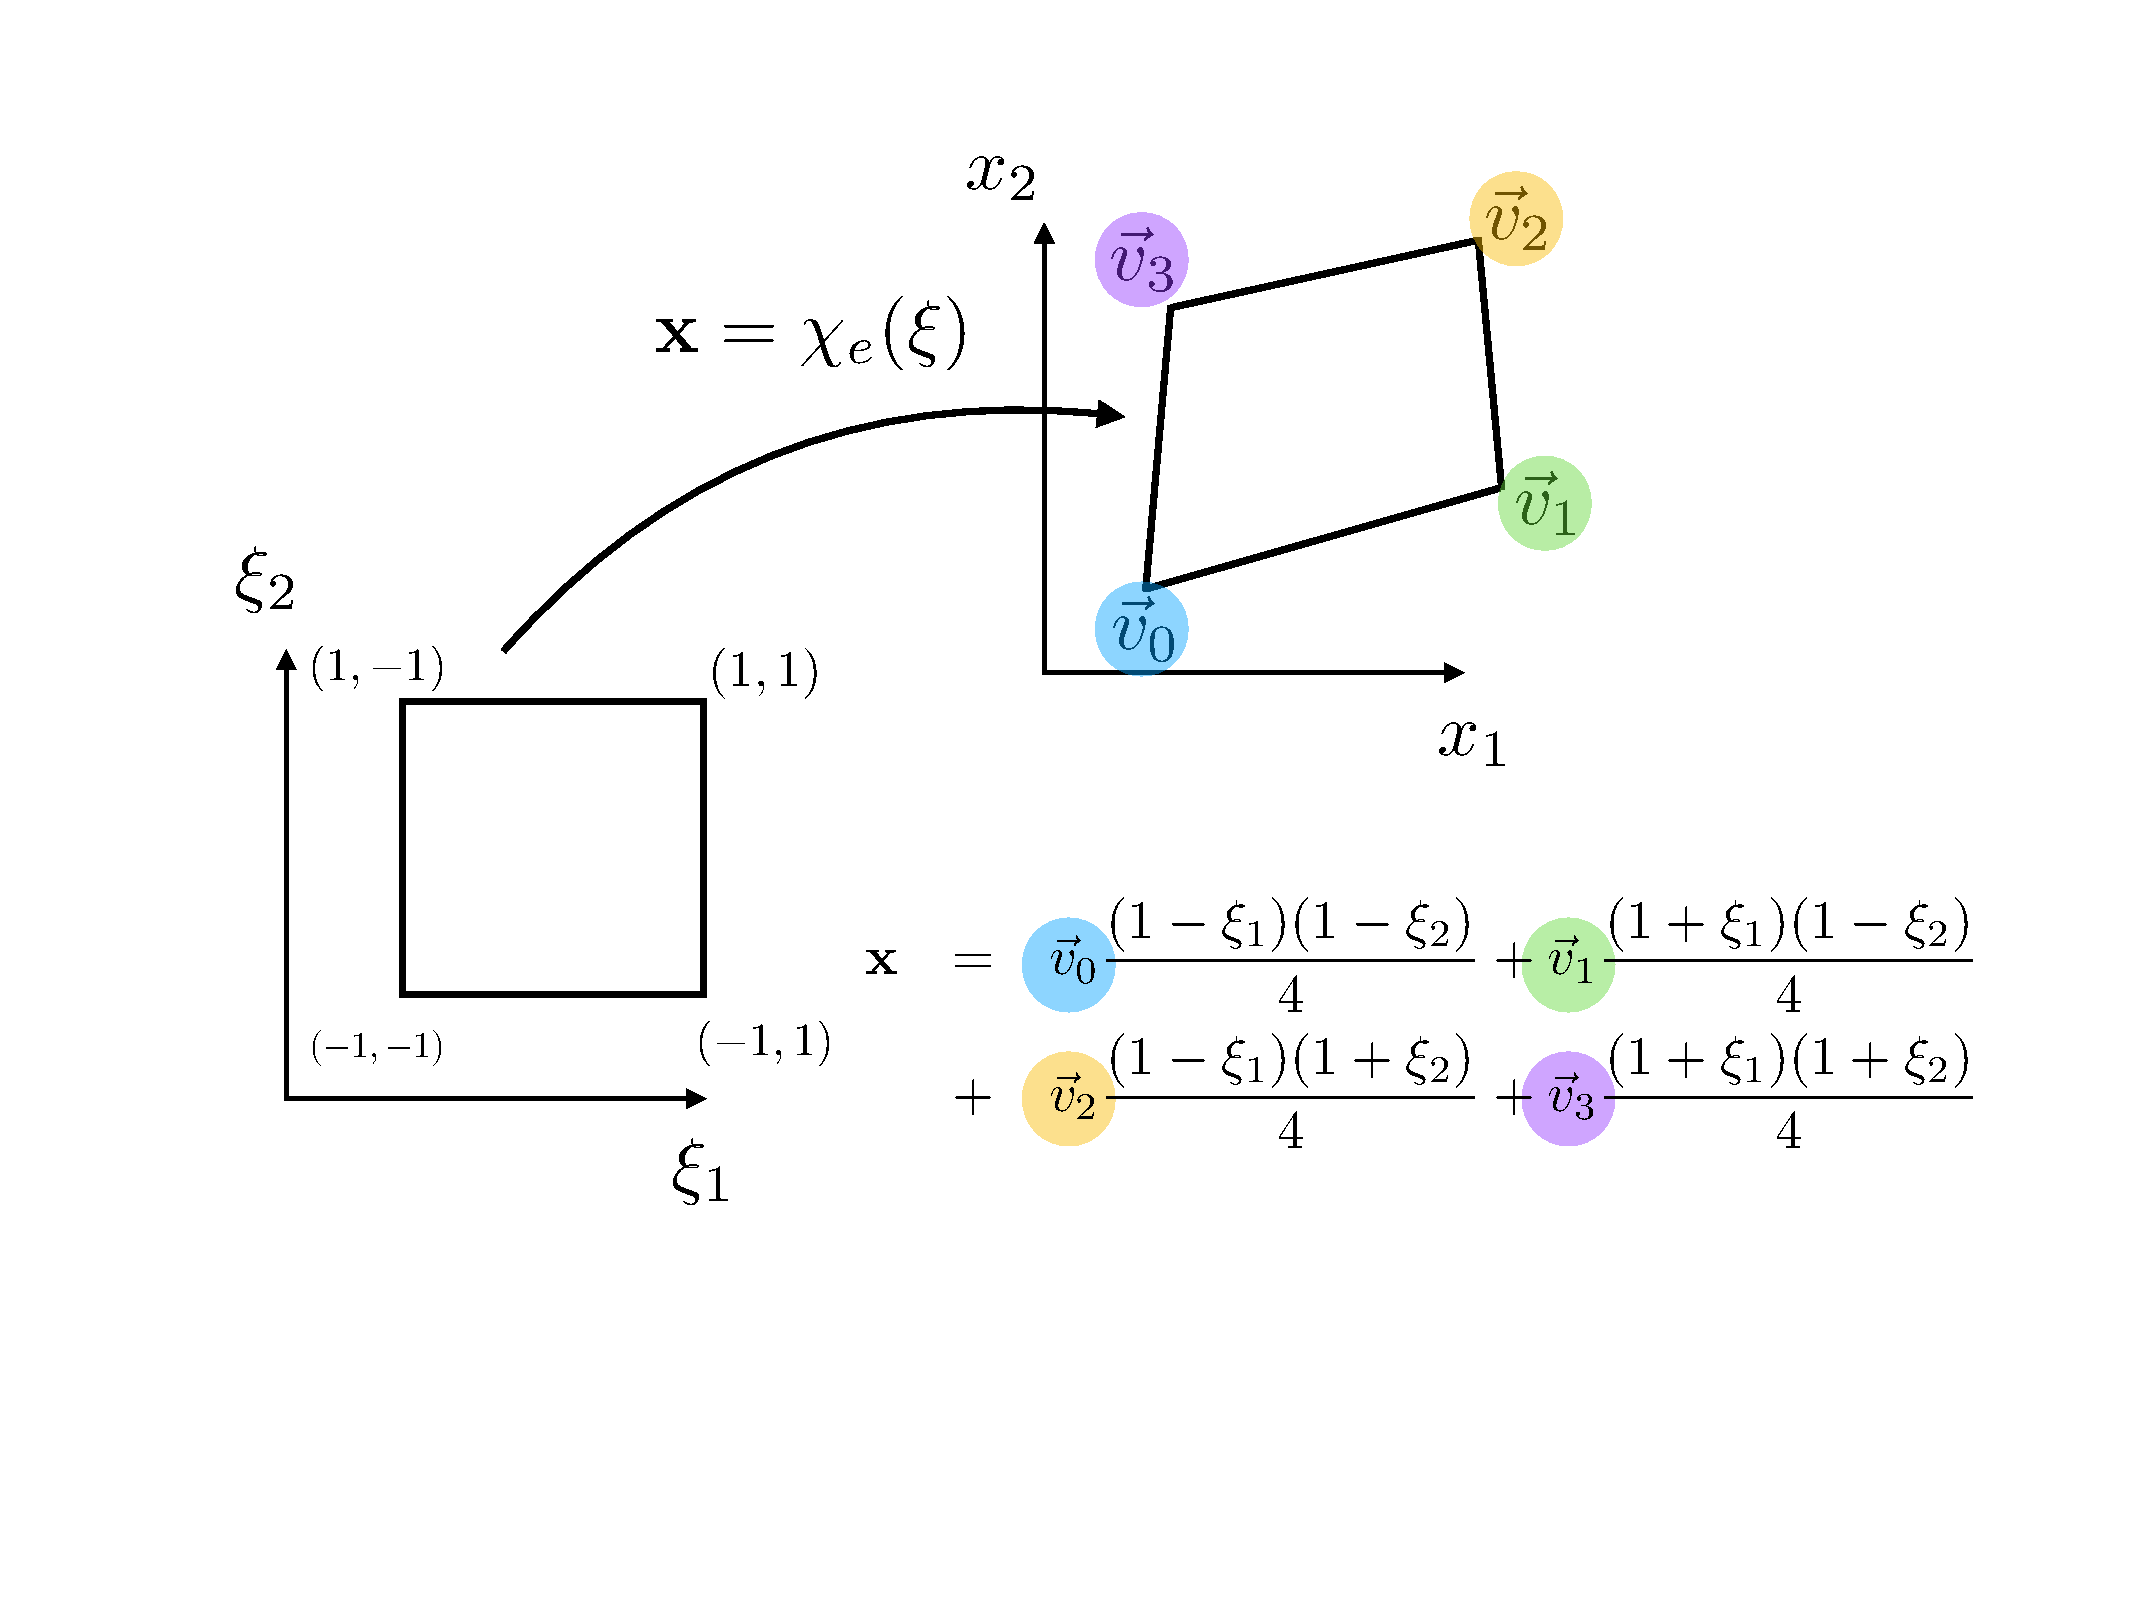
\includegraphics[width=6in]{img/planarmap.pdf}
\caption{Reference space to world space mapping of a 2D quadrilateral to a straight-sided (2D) quadrilateral in the plane via a bi-linear (i.e., $Q(1)$) mapping.}
\label{spatialdomains:planarmap}
\end{figure}

In the case of segments, this mapping function $\chi(\vec{\xi})$ is a function of one variable and is merely an affine mapping.  In two dimensions, the 
mapping of a straight-sided triangle is a linear mapping (i.e., P(1) in the language of traditional finite elements -- a total degree $k=1$ space) and
the mapping of a straight-sided quadrilateral is a bi-linear mapping (i.e, Q(1) in the language of traditional finite elements -- a degree $k=1$ map along each
coordinate direction combined through tensor-product).  In three dimensions, the mapping of a planar-sided tetrahedron is also a linear mapping, the
mapping of a planar-sided hexahedron is a tri-linear mapping, and the prism and pyramid are mathematically somewhere in-between these two canonical
types as given in \cite{KaSh05}.  The key point is that in the case of straight-sided (or planar-sided) elements, the mapping between reference space and
world space can be deduced solely based upon the vertex positions.  Furthermore in these cases, 
as denoted in Figure \ref{spatialdomains:planarmap}, the form of the mapping function is solely determined by type (shape) of the element.  If
only planar-sided elements are used, pre-computation involving the mapping functions can be done so that when vertex value information is available,
all the data structures can be finalized.  

As presented in \ref{KaSh05}, there are many components of {\nek} that capitalize on the geometric nature of the basis functions we use.  We often
speak in terms of vertex modes, edge modes, face modes and internal modes -- i.e., the coefficients that provide the weighting of vertex basis functions,
edge basis functions, etc.  It is beyond the scope of this developer guide to go into all the mathematical details of their definitions, etc.  However, we do 
want to point out a few common developer-level features that are important.   In the case of straight-sided (planar-sided) elements, the aforementioned
mapping functions can be fully described by vertex basis functions.  The real benefit of this approach (of connecting the mapping representation with a
geometric basis) is seen when moving to curved elements.

Consider Figure \ref{spatialdomains:curvemap} in which we modify the example given above to accommodate on curved edge.  From the 
mathematical perspective, we know that the inclusion of this (quadratic) edge will require our mapping function to now be in $Q(2)$.  If we were
not to use the fact that our basis is geometric in nature, we would be forced to form a Vandermonde system for a set of coefficients used
to combine the tensor-product quadratic functions (nine basis functions in all), and use the five pieces of information available to us (the four
vertex values and the one point $\vec{c}_0$ that informs the curve on edge $1$.   As shown in Figure \ref{spatialdomains:curvemap}, we would
expect that this updated (to accommodate a curved edge) mapping function to consist of the bi-linear mapping 
function with an additional term $C_1(\xi_1,\xi_2)$ that encompasses the new curvature information.  

\begin{figure}[htb]
\centering
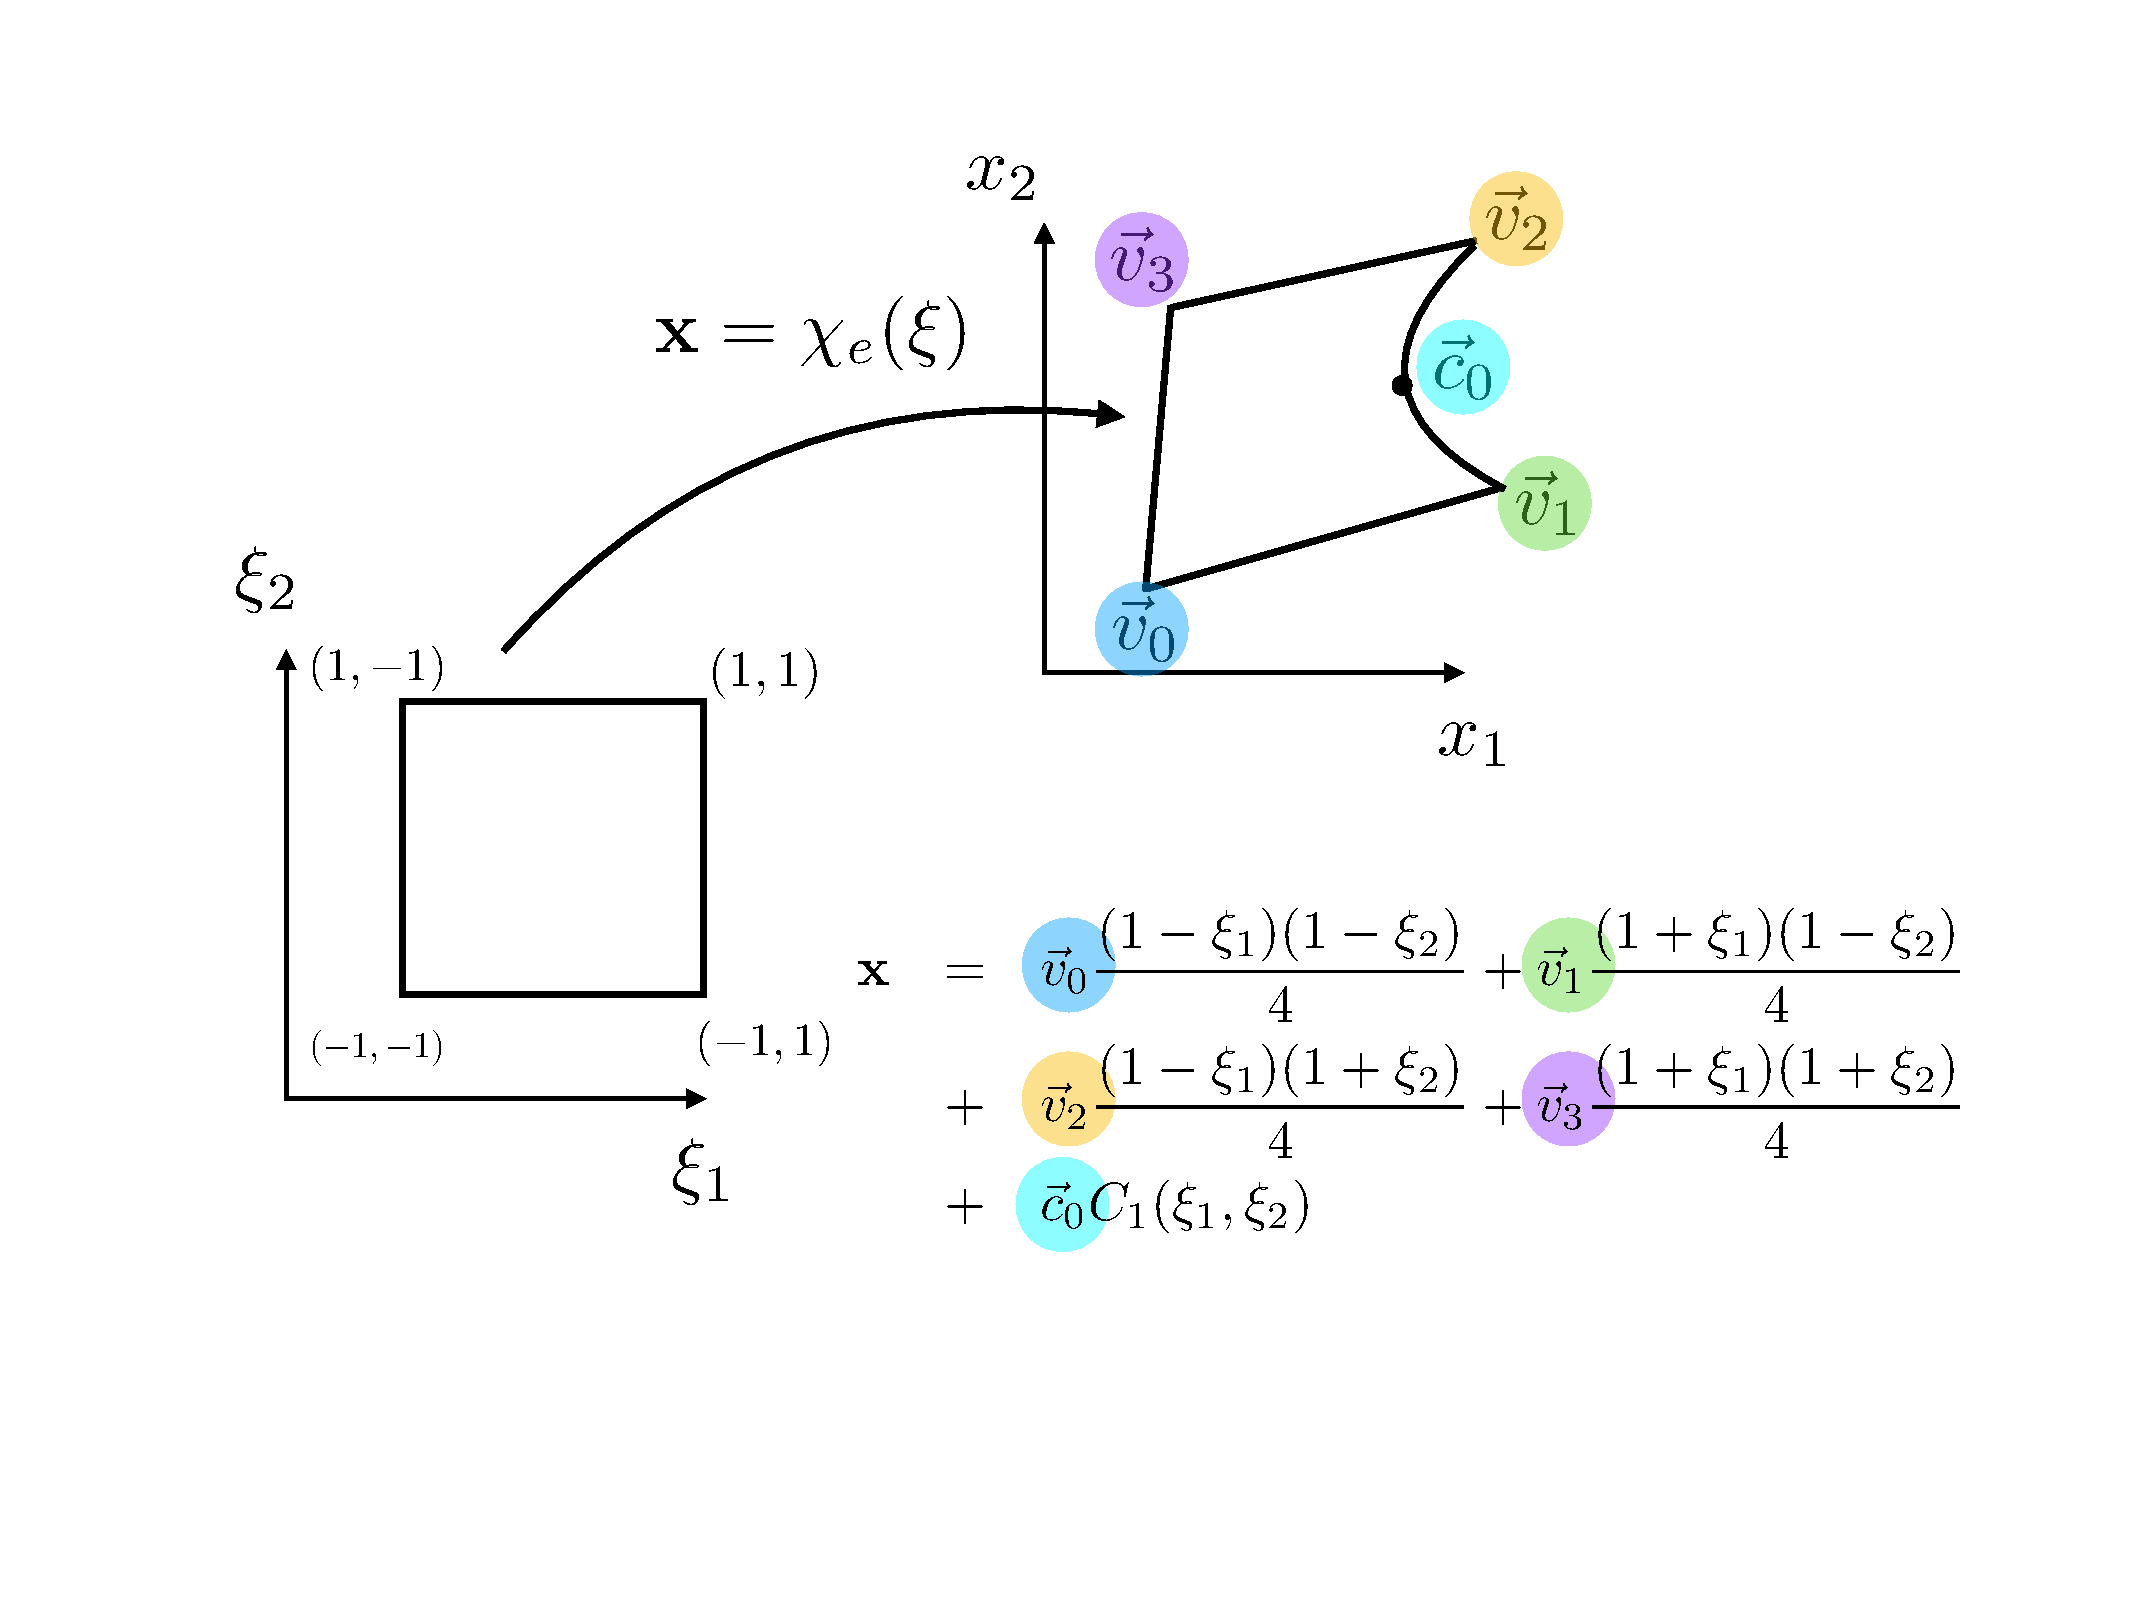
\includegraphics[width=6in]{img/curvemap.pdf}
\caption{Reference space to world space mapping of a 2D quadrilateral to a curve (2D) quadrilateral in the plane via a bi-quadratic (i.e., $Q(2)$) mapping.}
\label{spatialdomains:curvemap}
\end{figure}

The basis we use, following \cite{KaSh05}, allows us to precisely specify $C_1(\xi_1,\xi_2)$ using the edge basis function associated with edge $1$, and
to use the point value $\vec{c}_0$ to specify the coefficient to be used.  In the figure, we assume that the form of the function is collocating, but in practice
it need not be so.  

In practice, edge (and face) information can be given either as a set of point positions in world space that correspond to a particular point distribution 
in the reference element (i.e., evenly-spaced points or GLL points) or modal information corresponding to the geometric basis we use internally.  Our
geometric file formats assume the former -- that curve information is provided to us as physical values at specified positions from which we infer (calculate)
the modal values and store these values within SpatialDomain data structures.

Assuming we now have, for each element, a way of specifying the mapping function $\chi(\vec{\xi})$, we can now move to how we compute the geometric 
factors for regular as well as for deformed mappings. 
We use the term ``regular mappings" to refer to mappings from reference space elements to world space elements with the same dimension.  For instance, a 
collection of triangles that lie in a plane can be represented by vertex coordinates that an only 2-tuples and the mappings between the reference space
triangle the and world space triangle does not need to consider a larger embedded dimension.  This was a fundamental assumption of the original
Nektar code:  segments lived on the 1D line, triangles and quadrilaterals lived on the 2D plane and that hexahedra, tetrahedra, etc., lived in the 3D 
volume.   When redesigning {\nek}, we purposefully enabled geometric entities to live in a high-dimensional embedding space, different from their
parameterized dimension.  For instance, in {\nek}, it is possible to define segment expansions (functions that live over one dimensional parameterized
curves) that are embedded in 3D.  The same is true for quadrilaterals and triangles -- although their parameterized dimension is two, both may live in
a higher dimensional embedding space and thus represent a {\em manifold} of co-dimension one in that space.  For mappings that maintain the
co-dimension is the opposite of the dimension (i.e., quadrilateral in a plane represented by vertices with two coordinates mapped to a two parameter 
reference quadrilateral), we keep to the mapping conventions originally outlined in \cite{KaSh05} and denote these mapping operations in the code by the enumerated 
value {\em Regular}; for mappings in which the co-dimension is greater than zero, we following the modified convention outlined in \cite{CantwellYKPS14} and denote
these mapping operations in the code by the enumerated value {\em Deformed}.

\subsection{Regular Mappings: Geometric Factors}

Following \cite{KaSh05}, we assume that the vertex positions of an element in world space are given by $\vec{x} = x_i$ and that our reference space
coordinates are given by $\vec{\xi} = \xi_j$, there $i \text{ and } j$ run from zero to $dim-1$ where $dim$ is the parameter dimension of the element (e.g.
for a triangle, $dim = 2$).

The Jacobian (matrix) is correspondingly defined as:

\begin{equation} \label{eqn:jacobianmat}
{\bf J} = \frac{\partial x_i}{\partial \xi_j}.
\end{equation}

Note that this matrix is always square, but also note that it is not always constant across an element.  Only in special cases such as the 
linear mapping of triangles and tetrahedra does the Jacobian matrix reduce to a constant (matrix) over the entire element.  In general, 
this matrix can be evaluated at any point over the element for which it is constructed.

There are two (high-level) times in which this information is needed: when computing derivatives and when computing
integrals.  When computing derivatives, we employ the chain rule for differentiation, which in Einstein notation is given by the following expression:

$$
\frac{\partial}{\partial x_i} = \frac{\partial \xi_j}{\partial x_i} \frac{\partial}{\partial \xi_j}.
$$

Note that this expression requires the reciprocal of the expression above -- that is, ${\bf J}^{-1}$.  The polynomial mappings we use in {\nek}
are defined in terms of their forward mappings (reference to world).  If the determinant of the mapping is non-zero, the inverse of the mapping
exists but is not available analytically (except is special cases).  As a consequence, we in general limit the places at which we compute
the inverse of the Jacobian.  Typically, the quadrature point positions are the places at which you need these values (since it as at these
points we take physical space derivates and then use integration rules to construct weak form operators).  Thus, procedurally, we do the following:

\begin{enumerate}
\item For a given element, compute the Jacobian matrix using the expression given in Equation \ref{eqn:jacobianmat} for each quadrature point
position on the element (or for any points positions within an element at which it is needed).
\item Explicitly form the inverse of the matrix at each point position.
\end{enumerate}

Because we accomplish the inversion of the Jacobian matrix at particular positions, this introduces an approximation to this computation.
Although the inverse Jacobian matrix can be computed exactly at each point -- when we then correspondingly use this information 
in the inner product over an element -- we are in effect assuming that we are using a polynomial interpolative projection of this operator.
The approximation error is introduced at the point of our quadrature approximation.  Although the forward mapping is polynomial and hence
we could find a polynomial integration rule and number of points/weights to integrate our bilinear forms exactly, our use of the inverse
mapping in our bilinear forms means that we can only approximate our integrals.  From our experiments, the impact of his is negligible
in most cases, and only becomes in a concern in highly curved geometries.  In such cases, over-integration might be requires to minimize
the errors introduced due this approximation.

The other place at which we need the Jacobian matrix is to compute its determinant to be used in integration.  The determinant of the Jacobian
matrix (sometimes also called ``the Jacobian" of the mapping) provides us the scaling of the metric terms used in integration.  In all our
computations, we assume that the determinant of the Jacobian matrix is strictly positive.   In the area of mesh generation, the value 
of the determinant is used to estimate how good or bad the quality of the mapping is -- in effect, if you have reasonable elements in your mesh.
Negative Jacobian elements are inadmissible but even elements with small Jacobian determinants might cause issues.   At
the level of the library and solvers, we assume that these issues have been addressed by the user prior to attempting to run {\nek}
solvers and interpret their results.


\subsection{Deformed Mappings: Geometric Factors}

Following \cite{CantwellYKPS14}, we again assume that the vertex positions of an element in world space are given by $\vec{x} = x_i$ and that our reference space
coordinates are given by $\vec{\xi} = \xi_j$, there $i$ runs from zero to $dim-1$ where $dim$ is the embedding dimension and $j$ runs from zero to $M-1$ where $M$
is the parameter dimension of the element (e.g.for a triangle on a manifold embedded in 3D with vertex values in 3D, $dim = 3$ whilst $M=2$).

The Jacobian (matrix) is correspondingly defined as:

\begin{equation} \label{eqn:jacobianmat}
{\bf J} = J^i_j = \frac{\partial x_i}{\partial \xi_j}.
\end{equation}

In this case, we use the notational conventions of \cite{Ar89} which delineate covariant and contravariant forms. In general, this matrix is not square, 
also also note that it is not always constant across an element.  In general, this matrix can be evaluated at any point over the element for which it is constructed.
The metric tensor related to this transformation can be formed as:

$$
{\bf g} = {\bf J}{\bf J}^T
$$

\noindent and the Jacobian factor associated with this mapping is then given by:

$$
g = \det{\bf g}.
$$

Because various mappings are necessary when dealing with covariant and contravariant vectors, we have encapsulated all these routines 
into the directory GlobalMapping (see Chapter \ref{chapter:globalmapping}).  At this stage, we do not implement general Piola transformations \cite{McRaeBMHC} that further respect $H(div)$ and $H(curl)$ constraints on these mappings
as would be needed in solid mechanics or electromagnetics; however, there is nothing inherent within the {\nek} framework that would preclude someone from
adding these additional features as necessary.



%
%
\section{The Fundamental Data Structures within SpatialDomains}
\label{sec:spatialdomains-datastructures}

As mentioned earlier, in almost all object-oriented languages (which includes $C++$), there exists the concepts of {\em class attributes} and {\em object attributes}.   For a summary of attributes and access patterns, please review Section \ref{sec:stdregions-datastructures}.
Within the SpatialDomains directory of the library, there exists a class inheritance hierarchy designed to try to encourage re-use of core
algorithms (while simultaneously trying to minimize duplication of code).  We present this class hierarchy in Figure \ref{spatialdomains:geomtree}.


\begin{figure}[htb]
\centering
\includegraphics[width=6in]{img/geomtree.pdf}
\caption{Class hierarchy derived from Geometry, the base class of the SpatialDomains Directory.}
\label{spatialdomains:geomtree}
\end{figure}

At its core, the items contained within SpatialDomains are meant to represent the mapping of StdRegion information into world-space.  The various attributes contained herein related to this geometric (mesh, curvature and mapping) information.  The various private, protected and public data members contained within StdRegions are provided in the subsequent sections.


%%%%%%%%%%%%%%%%%%%%%%%%%%%%%%%%%%%%%%%%
\subsection{Variables at the Level of Geometry}

\paragraph{Private:}

\paragraph{Protected:}

\paragraph{Public:}


%%%%%%%%%%%%%%%%%%%%%%%%%%%%%%%%%%%%%%%%
\subsection{Variables at the Level of Geometry\$D for various Dimensions}

\paragraph{Private:}

\paragraph{Protected:}

\paragraph{Public:}

%%%%%%%%%%%%%%%%%%%%%%%%%%%%%%%%%%%%%%%%
\subsection{Variables at the Level of Shape-Specific Geometry Information}

\paragraph{Private:}

\paragraph{Protected:}

\paragraph{Public:}



%%%%%%%%%%%%%%%%%%%%%%%%%%%%%%%%%%%%%
\subsection{Reference to World-Space Mapping}

%%%%%%%%%%%%%%%%%%%%%%%%%%%%%%%%%%%%%
\subsubsection{Geometry}


%%%%%%%%%%%%%%%%%%%%%%%%%%%%%%%%%%%%%
\subsubsection{GeomFactors}




%%%%%%%%%%%%%%%%%%%%%%%%%%%%%%%%%%%%%
\subsection{MeshGraph}
%
%
\section{The Fundamental Algorithms within SpatialDomains}

As stated in the introduction, this section of this guide is structured in question-answer form.  This is not meant to capture every possible
question asked of us on the {\nek} users list; however, this set of (ever-growing) questions are meant to capture the ``big ideas'' that developers 
want to know about how SpatialDomains work and how they can be used.  

In this section, we will through question and answer format try to cover the following basic algorithmic concepts that are found within 
the SpatialDomains part of the library:

\begin{itemize}
\item xx
\end{itemize}

With the big ideas in place, let us now start into our questions.

\paragraph{Question:}



%%%%%%%%%%%%%%%%%%%%%%%%%%%%%%%
\chapter{Inside the Library: LocalRegions}
\label{chap:localregions}


In this chapter, we walk the reader through the different components
of the LocalRegions Directory.  We begin with a discussion of the
mathematical fundamentals, for which we use the book by Karniadakis
and Sherwin \cite{KaSh05} as our principle reference.  We then provide
the reader with an overview of the primary data structures introduced
within the LocalRegions Directory (often done through C++ objects),
and then present the major algorithms -- expressed as either object
methods or functions -- employed over these data structures.

%
\section{The Fundamentals Behind LocalRegions}

The idea behind local regions is strongly connected to that of standard regions, but from the top-down perspective.  As an example: in standard regions, we only had to consider one type of triangle, the one that is straight-sided, right-angled, and whose principle horizontal and vertical sides where aligned with the coordinate axes.  Of course, meshes of elements consist of elements that may are may not be right-angled, planar-sided, etc.  The starting point for us is the question of how to build build basis functions that exist of a {\em world-space} element -- that is, an element whose vertex positions lie in the engineering (PDE) coordinate system of interest.  Such an expansion is a local region.  In {\nek}, each local region {\em is-a} standard region and {\em has-a} spatial domain data structure.  The local region inherits common expansion methods from its standard region parent, and it uses its spatial domain information to specialize its operators to its local coordinate system.


%
%
\section{The Fundamental Data Structures within LocalRegions}

As mentioned earlier, in almost all object-oriented languages (which includes $C++$), there exists the concepts of {\em class attributes} and {\em object attributes}.   For a summary of attributes and access patterns, please review Section \ref{sec:stdregions-datastructures}.
Within the LocalRegions directory of the library, there exists a class inheritance hierarchy designed to try to encourage re-use of core
algorithms (while simultaneously trying to minimize duplication of code).  We present this class hierarchy in Figure \ref{localregions:localclasstree}.


\begin{figure}[htb]
\centering
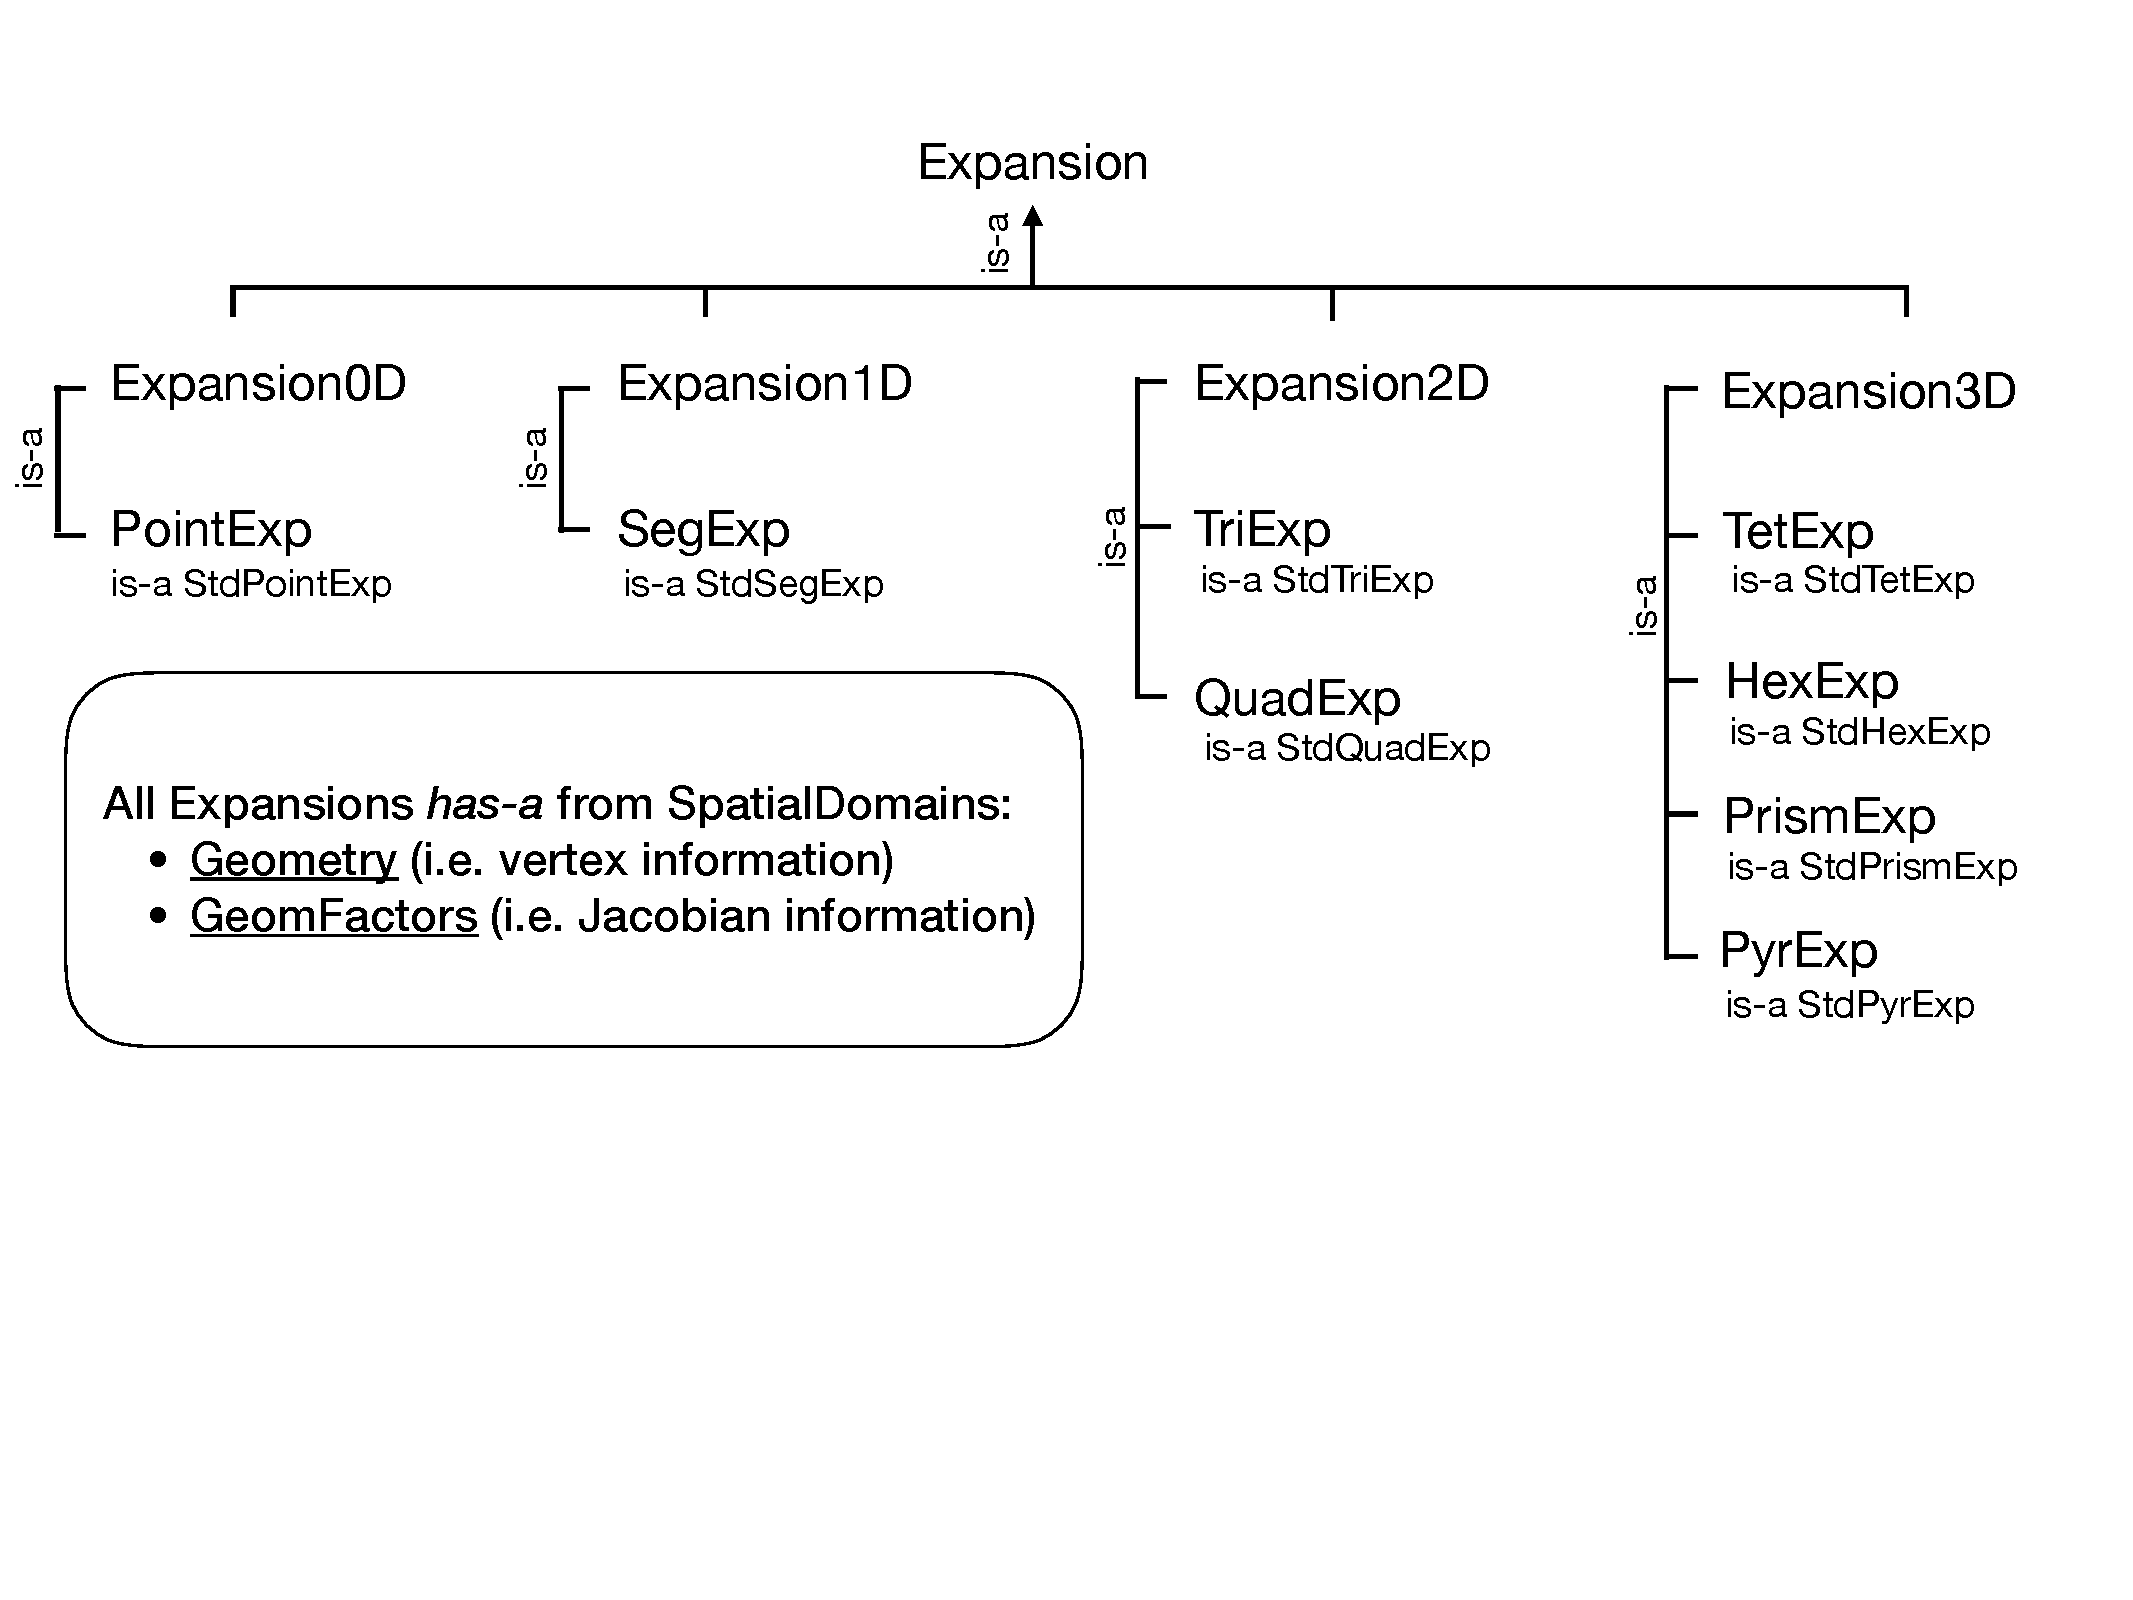
\includegraphics[width=6in]{img/expansiontree.pdf}
\caption{Class hierarchy derived from Expansion, the base class of the LocalRegions Directory.}
\label{localregions:localclasstree}
\end{figure}

As is seen in Figure \ref{stdregions:localclasstree}, the LocalRegions hierarchy consists of three levels:  the base level from which all
LocalRegion objects are derived is Expansion.   This object is then specialized by dimension, yielding Expansion0D, 
Expansion1D, Expansion2D and Expansion3D.  The dimension-specific objects are then specialized based upon
shape.  

The object attributes (variables) at various levels of the hierarchy can be understood in light of Figure \ref{stdregions:stdexpansion}.
At its core, an expansion is a means of representing a function over a world-space region evaluated at a collection of point positions.
The various data members hold information to allow all these basic building blocks to be specified.  Many of the attributes are 
inherited from StdRegions as they are not unique to LocalRegions; however, each LocalRegion Expansion is uniquely defined based
upon its geometric factors (which it stores via SpatialDomain information).


\begin{figure}[htb]
\centering
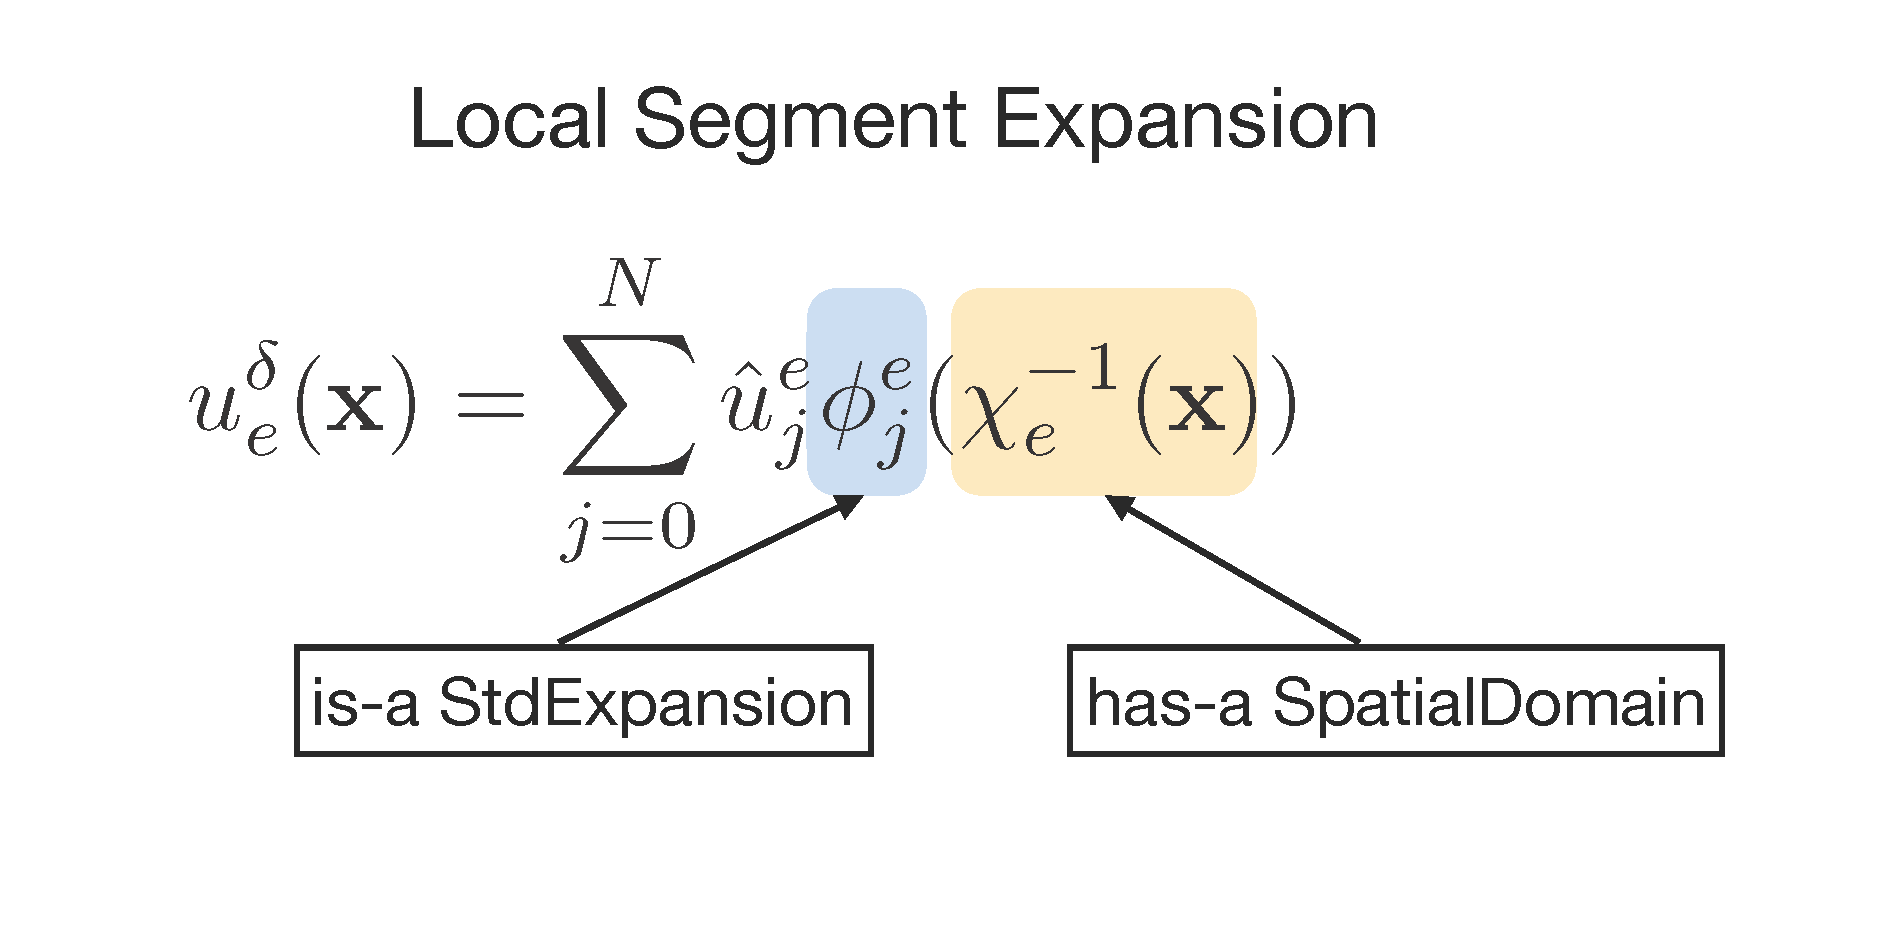
\includegraphics[width=6in]{img/LocalExpansion.png}
\caption{Diagram to help understand the various data members (object attributes) contained within LocalRegions and how they connect with the mathematical representation presented earlier.  Recall that a LocalRegion {\em is-a} StdRegion and {\em has-a} SpatialDomain.}
\label{localregions:localexpansion:stdexpansion}
\end{figure}

The various private, protected and public data members contained within LocalRegions are provided in the subsequent sections.

%%%%%%%%%%%%%%%%%%%%%%%%%%%%%%%%%%%%%%%%
\subsection{Variables at the Level of Expansion}

\paragraph{Private:}

There are private methods but no private data members within Expansion.

\paragraph{Protected:}

As discussed above, the primary data in LocalRegions that distinguishes it from StdExpansions is the {\em has-a} relationship with SpatialDomains, given by the following:

\begin{itemize}
\item SpatialDomains::GeometrySharedPtr  \verb+m_geom+
%
\item SpatialDomains::GeomFactorsSharedPtr \verb+m_metricinfo+
%
\item MetricMap \verb+m_metrics+
\end{itemize}


\paragraph{Public:}

There are public methods but no public data members within Expansion.


%%%%%%%%%%%%%%%%%%%%%%%%%%%%%%%%%%%%%%%%
\subsection{Variables at the Level of Expansion\$D for various Dimensions}
\paragraph{Private:}

\paragraph{Protected:}

\paragraph{Public:}


%%%%%%%%%%%%%%%%%%%%%%%%%%%%%%%%%%%%%%%%
\subsection{Variables at the Level of Shape-Specific Expansions}

\paragraph{Private:}

\paragraph{Protected:}

\paragraph{Public:}


%
%
\section{The Fundamental Algorithms within LocalRegions}

As stated in the introduction, this section of this guide is structured in question-answer form.  This is not meant to capture every possible
question asked of us on the {\nek} users list; however, this set of (ever-growing) questions are meant to capture the ``big ideas'' that developers 
want to know about how LocalRegions work and how they can be used.  

In this section, we will through question and answer format try to cover the following basic algorithmic concepts that are found within 
the LocalRegions part of the library:

\begin{itemize}
\item xx
\end{itemize}

With the big ideas in place, let us now start into our questions.

\paragraph{Question:}



%%%%%%%%%%%%%%%%%%%%%%%%%%%%%%%
\chapter{Inside the Library: Collections}

In this chapter, we walk the reader through the different components
of the Collections Directory.  We begin with a discussion of the
mathematical fundamentals, for which we use the book by Karniadakis
and Sherwin \cite{KaSh05} as our principle reference.  We then provide
the reader with an overview of the primary data structures introduced
within the Collections Directory (often done through C++ objects), and
then present the major algorithms -- expressed as either object
methods or functions -- employed over these data structures.

%
\section{The Fundamentals Behind Collections}

The concept of ``collections'' is that there are many operations that we (conceptually) accomplish on an element-by-element basis that can be aggregated together into a single operation.  The
basic idea is that whenever you see a piece of code that consists of a loop in which, in the body of the loop, you are accomplishing the same operation (e.g. function evaluation) based upon 
an input variable tied to the loop index -- you may be able to make the operation a ``collection''.  For instance, consider if you were given the following snippet of code in Matlab notation:
\vspace{-5mm}
\begin{verbatim}
     do j = 1:N,
          y(j) = dot(a,x(:,j))
     end
\end{verbatim}

\noindent where $y$ is a row vector of length $N$, $x$ is an $M \times N$ matrix and $a$ is a row vector of length $M$.  Note that in this code snipped, the
vector $a$ remains constant; only the vector $x$ involved in the dot product is changing based upon the index (i.e. selecting a column of the array).  
From linear algebra, you might recognize this as the way we accomplish the product of a row vector with a matrix -- we march through the matrix accomplishing
dot products.  Although these two things are equivalent mathematically, they are not equivalent computationally {\em from the perspective of computational efficiency}.   Most linear algebra operations within {\nek} are done using BLAS -- Basic Linear Algebra Subroutines -- a collection of specialized routines
for accomplishing Level 1 (single loop), Level 2 (double nested loop) and Level 3 (triple nested loop) operations.  A dot product is an example of a Level 1
BLAS operation;  A matrix-vector multiplication is an example of a Level 2 BLAS operation; and finally a matrix-matrix multiplication is an example of a Level 3
BLAS operation.  The general rule of thumb is that as you move up the levels, the operations can be made more efficient (using various algorithmic 
reorganization and memory layout strategies).  Hence when you see a loop over Level 1 BLAS calls (like in the above piece of code), you should always
ask yourself if this could be transformed into a Level 2 BLAS call.  Since the vector $a$ is not changing, this piece of code should be replaced with an
appropriate vector-matrix multiply.

As seen in StdRegions and LocalRegions, we often conceptually thing of many of our basic building block operations as being elemental.  We have 
elemental basis matrices, local stiffness matrices, etc.  Although it is correct to implement operations as an iterator over elements in which you accomplish
an action like evaluation (done by taking a basis evaluation matrix times a coefficient vector), this operation can be made more efficient by ganging all these
elemental operations together into a {\em collection}.  

As mentioned earlier, one of the caveats of this approach is that you must assume some level of consistency of the operation.  For instance, in the case of physical evaluations, you must assume that a collection consists of elements that are all of the same time, have the same basis number and ordering, and are evaluated at the same set of points -- otherwise the operation cannot be expressed as a single (basis) matrix multiplied by a matrix whose columns consist of the modes
of all the elements who have joined the collective operation.

As will be seen in the data structure and algorithms sections of this discussion, these assumptions lead us to two fundamental types of collections:  collections that live at the StdRegions level (i.e. collection operations that act on a group of elements as represented in reference space) and collections that live at the LocalRegions level (i.e. collection operations that act on a group of elements as represented in world space).
%
%
\section{The Fundamental Data Structures within Collections}
%
%
\section{The Fundamental Algorithms within Collections}

As stated in the introduction, this section of this guide is structured in question-answer form.  This is not meant to capture every possible
question asked of us on the {\nek} users list; however, this set of (ever-growing) questions are meant to capture the ``big ideas'' that developers 
want to know about how Collections work and how they can be used.  

In this section, we will through question and answer format try to cover the following basic algorithmic concepts that are found within 
the Collections part of the library:

\begin{itemize}
\item xx
\end{itemize}

With the big ideas in place, let us now start into our questions.

\paragraph{Question:}



%%%%%%%%%%%%%%%%%%%%%%%%%%%%%%%
\chapter{Inside the Library: MultiRegions}
\label{chap:multiregions}


In this chapter, we walk the reader through the different components
of the MultiRegions Directory.  We begin with a discussion of the
mathematical fundamentals, for which we use the book by Karniadakis
and Sherwin \cite{KaSh05} as our principle reference.  We then provide
the reader with an overview of the primary data structures introduced
within the MultiRegions Directory (often done through C++ objects),
and then present the major algorithms -- expressed as either object
methods or functions -- employed over these data structures.

%
\section{The Fundamentals Behind MultiRegions}

Up to now in the library, the various data structures and methods associated with standard regions, spatial domains and local regions are not 
specifically dictated by any particular numerical method.   In fact, at this stage, they can all be viewed in light of approximation theory.  With
local regions in place, we have a region in world space over which we can represent an expansion (i.e. linear combination of basis functions)
and form its derivatives and its integral.  It is at the level of MultiRegions that we now combine two fundamental concepts: the idea of a collection
of elements together to form a ``global" expansion and the idea of how these (local) elements communicate (in the sense of how does one form
approximations of a PDE of these collections of elements).   Hence MultiRegions is important because it gives us a way of dealing with general tessellation and
also because it is the first place at which we can connect to a specific numerical PDE approximation methods of choice (i.e. continuous Galerkin FEM methods,
discontinuous Galerkin finite volume methods, etc.).

Because MultiRegions is both about grouping of elements in space (to form a domain) and about solving PDEs over these domains, you will find two primary
collections of routines contained within the MultiRegions directory.  You will find things related to collections of elements:  ExpList (Expansion List), DisContField (discontinuous
field) and ConField (continuous field); and you will find objects related to the linear systems formed based upon the particular numerical method once selects (i.e. GlobalLinSys, 
which stands for Global Linear System).

At present, the {\nek} framework supports three types of numerical PDE discretizations for conservation laws:

\begin{itemize}
\item {\bf Discontinuous Galerkin Methods:} These weak-form (variational) methods do not require element continuity, but do put restrictions on the flux of information between elements.  In general, these methods can be thought of as being in the class of finite volume (FV) methods.  One feature of these methods that is often exploited computationally is that
many operations can be considered as elemental.   See \cite{CockburnKS,HesthavenW08} and references therein for a more complete summary.
%
\item {\bf Continuous Galkerin Methods:}  These weak-form (variational) methods require at least $C^0$ continuity.  Mathematically, there have been extensions to 
higher levels of continuity, e.g. Isogeometric Analysis  \cite{CottrellISO}, these are not implemented in {\nek} and would require further constraints on our SpatialDomain
representations than we currently accommodate.  In general, these methods can be thought of as being in the class of finite element methods (FEM).  Although 
these methods are technically (mathematically) formulated as global methods, their elemental construction and compact basis types allow for many local operations.
Many (but not all) of the linear system routines that are contained with the MultiRegions directory are focussed on this discretization type.
See \cite{Schwab, DevilleFM02,KaSh05}  and references therein for a more complete summary.
%
\item {\bf Flux Reconstruction Methods:}  These strong-form methods do not require element continuity, but like dG methods they impose restrictions on the flux of information between elements.  In general, these methods can be though of as being in the class of generalized finite difference (FD) or collocating methods. 
See  \cite{Kopriva,WitherdenVJ2016} and references therein for a more complete summary.
\end{itemize}

\paragraph{Assembly Map}



\begin{figure}[htb]
\centering
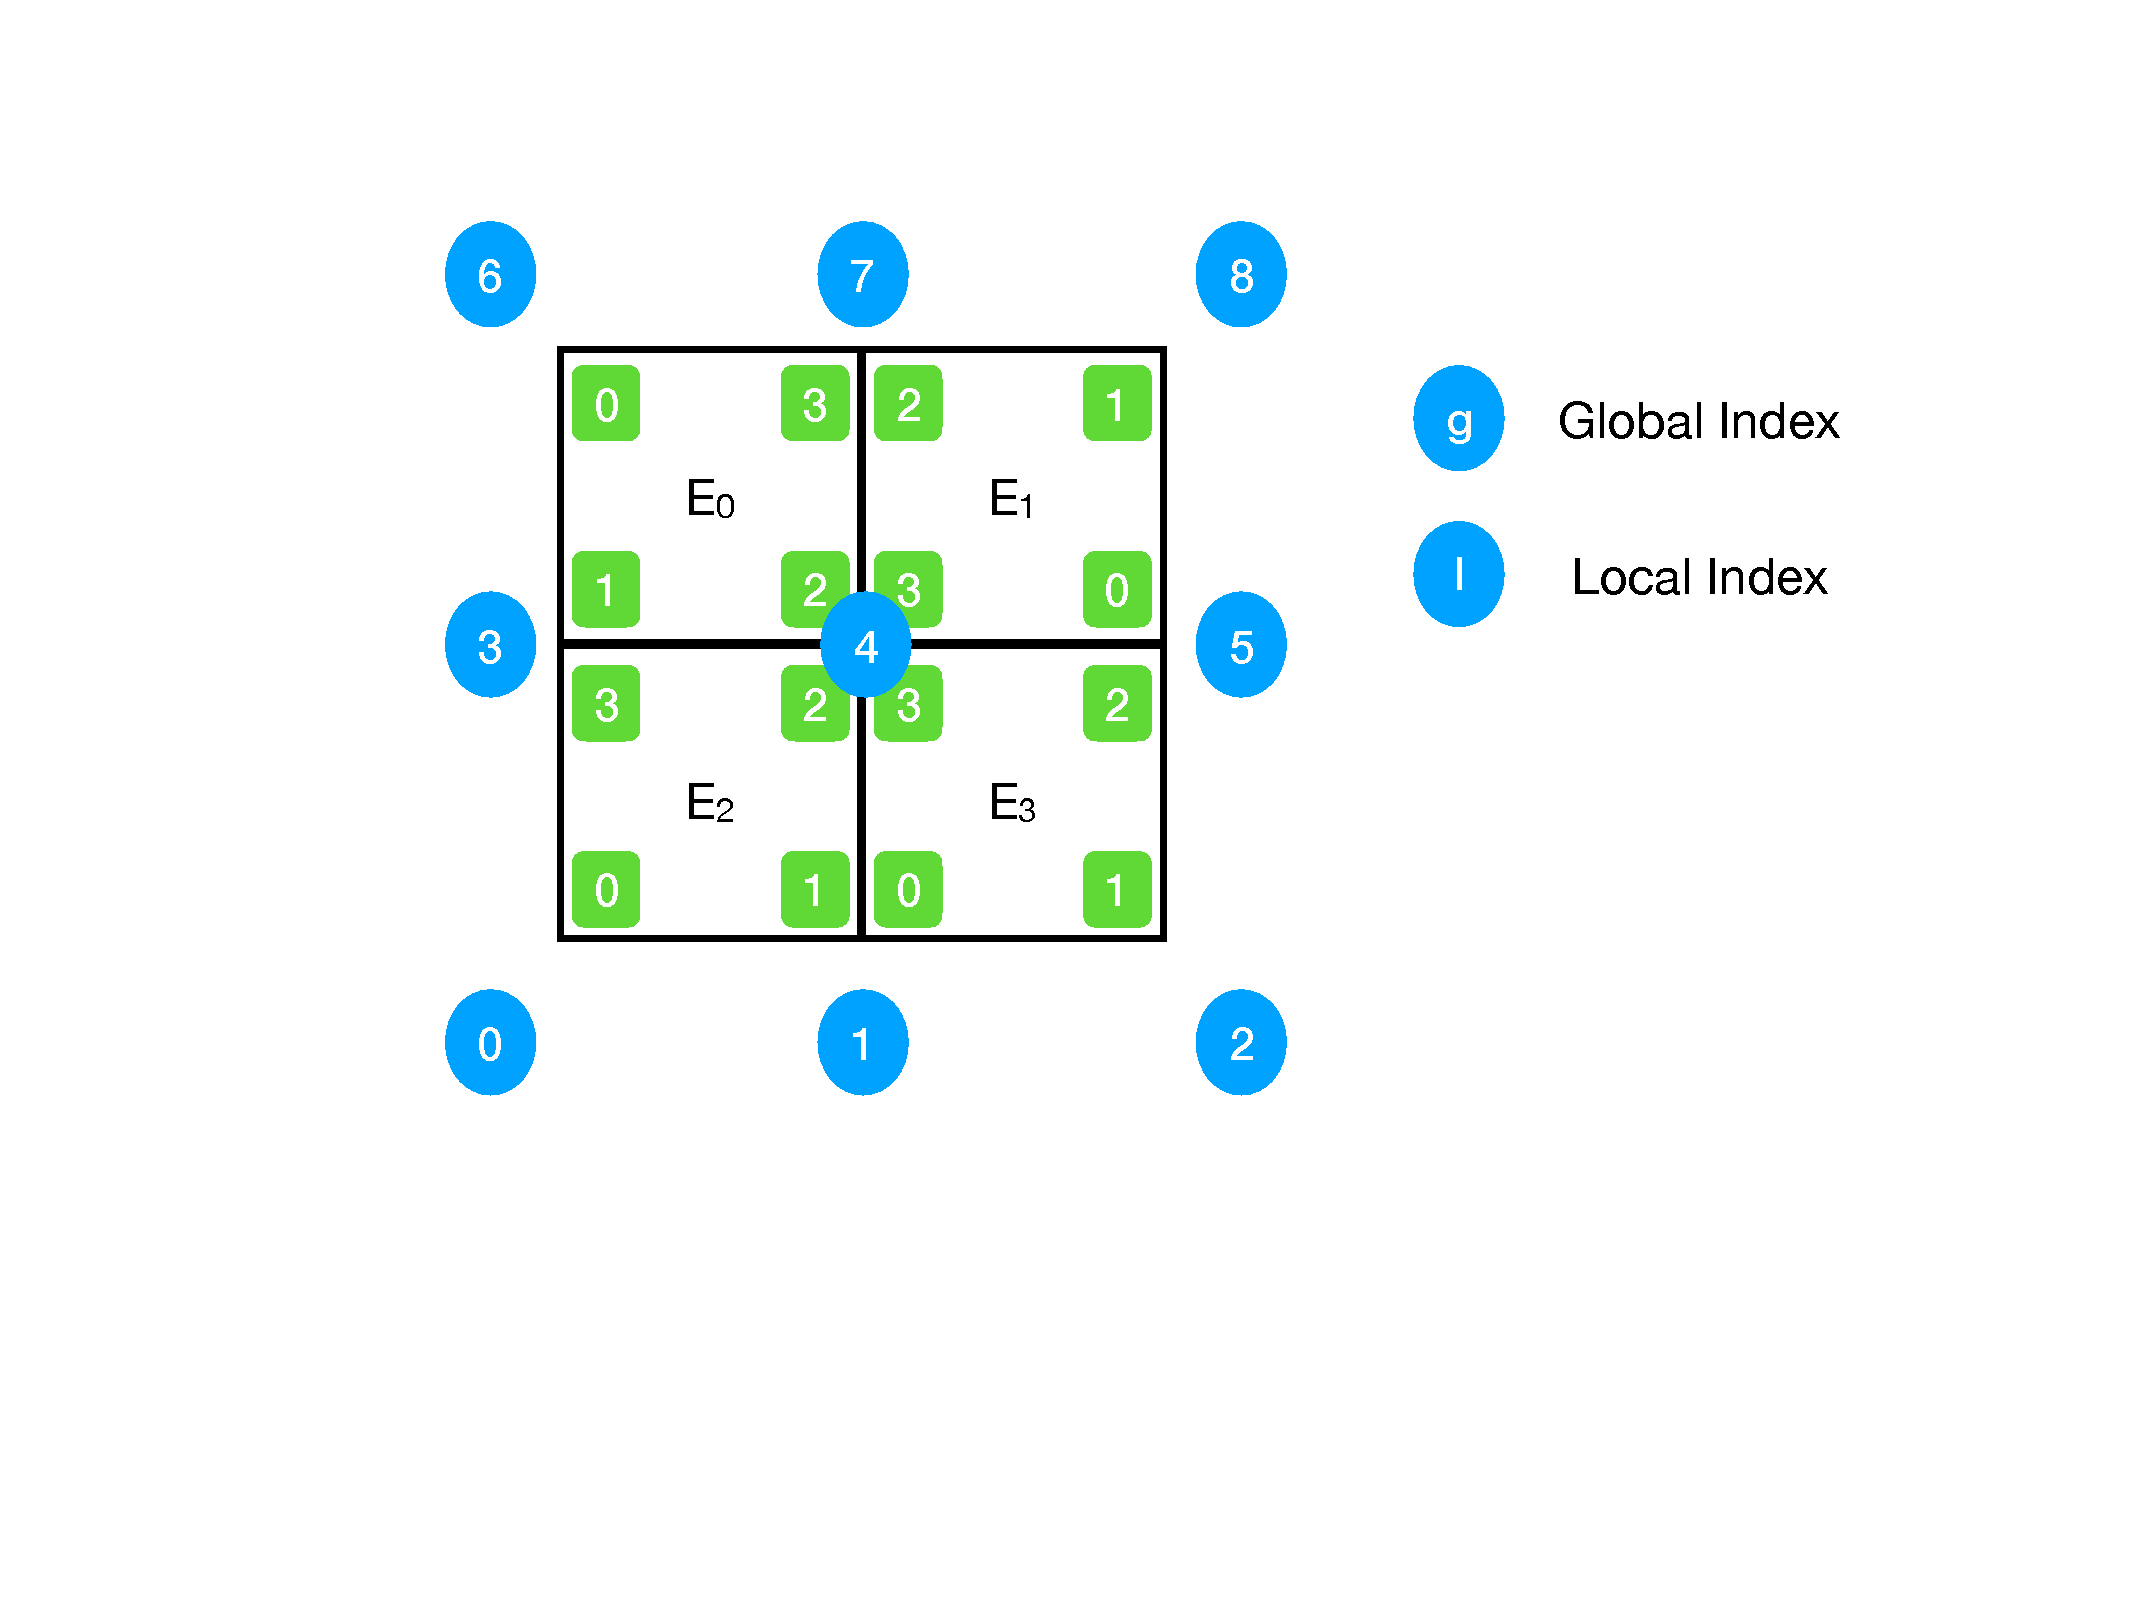
\includegraphics[width=4in]{img/Assembly1.pdf}
\caption{Diagram to help explain assembly.  UPDATE.}
\label{multiregions:assembly1}
\end{figure}


\begin{figure}[htb]
\centering
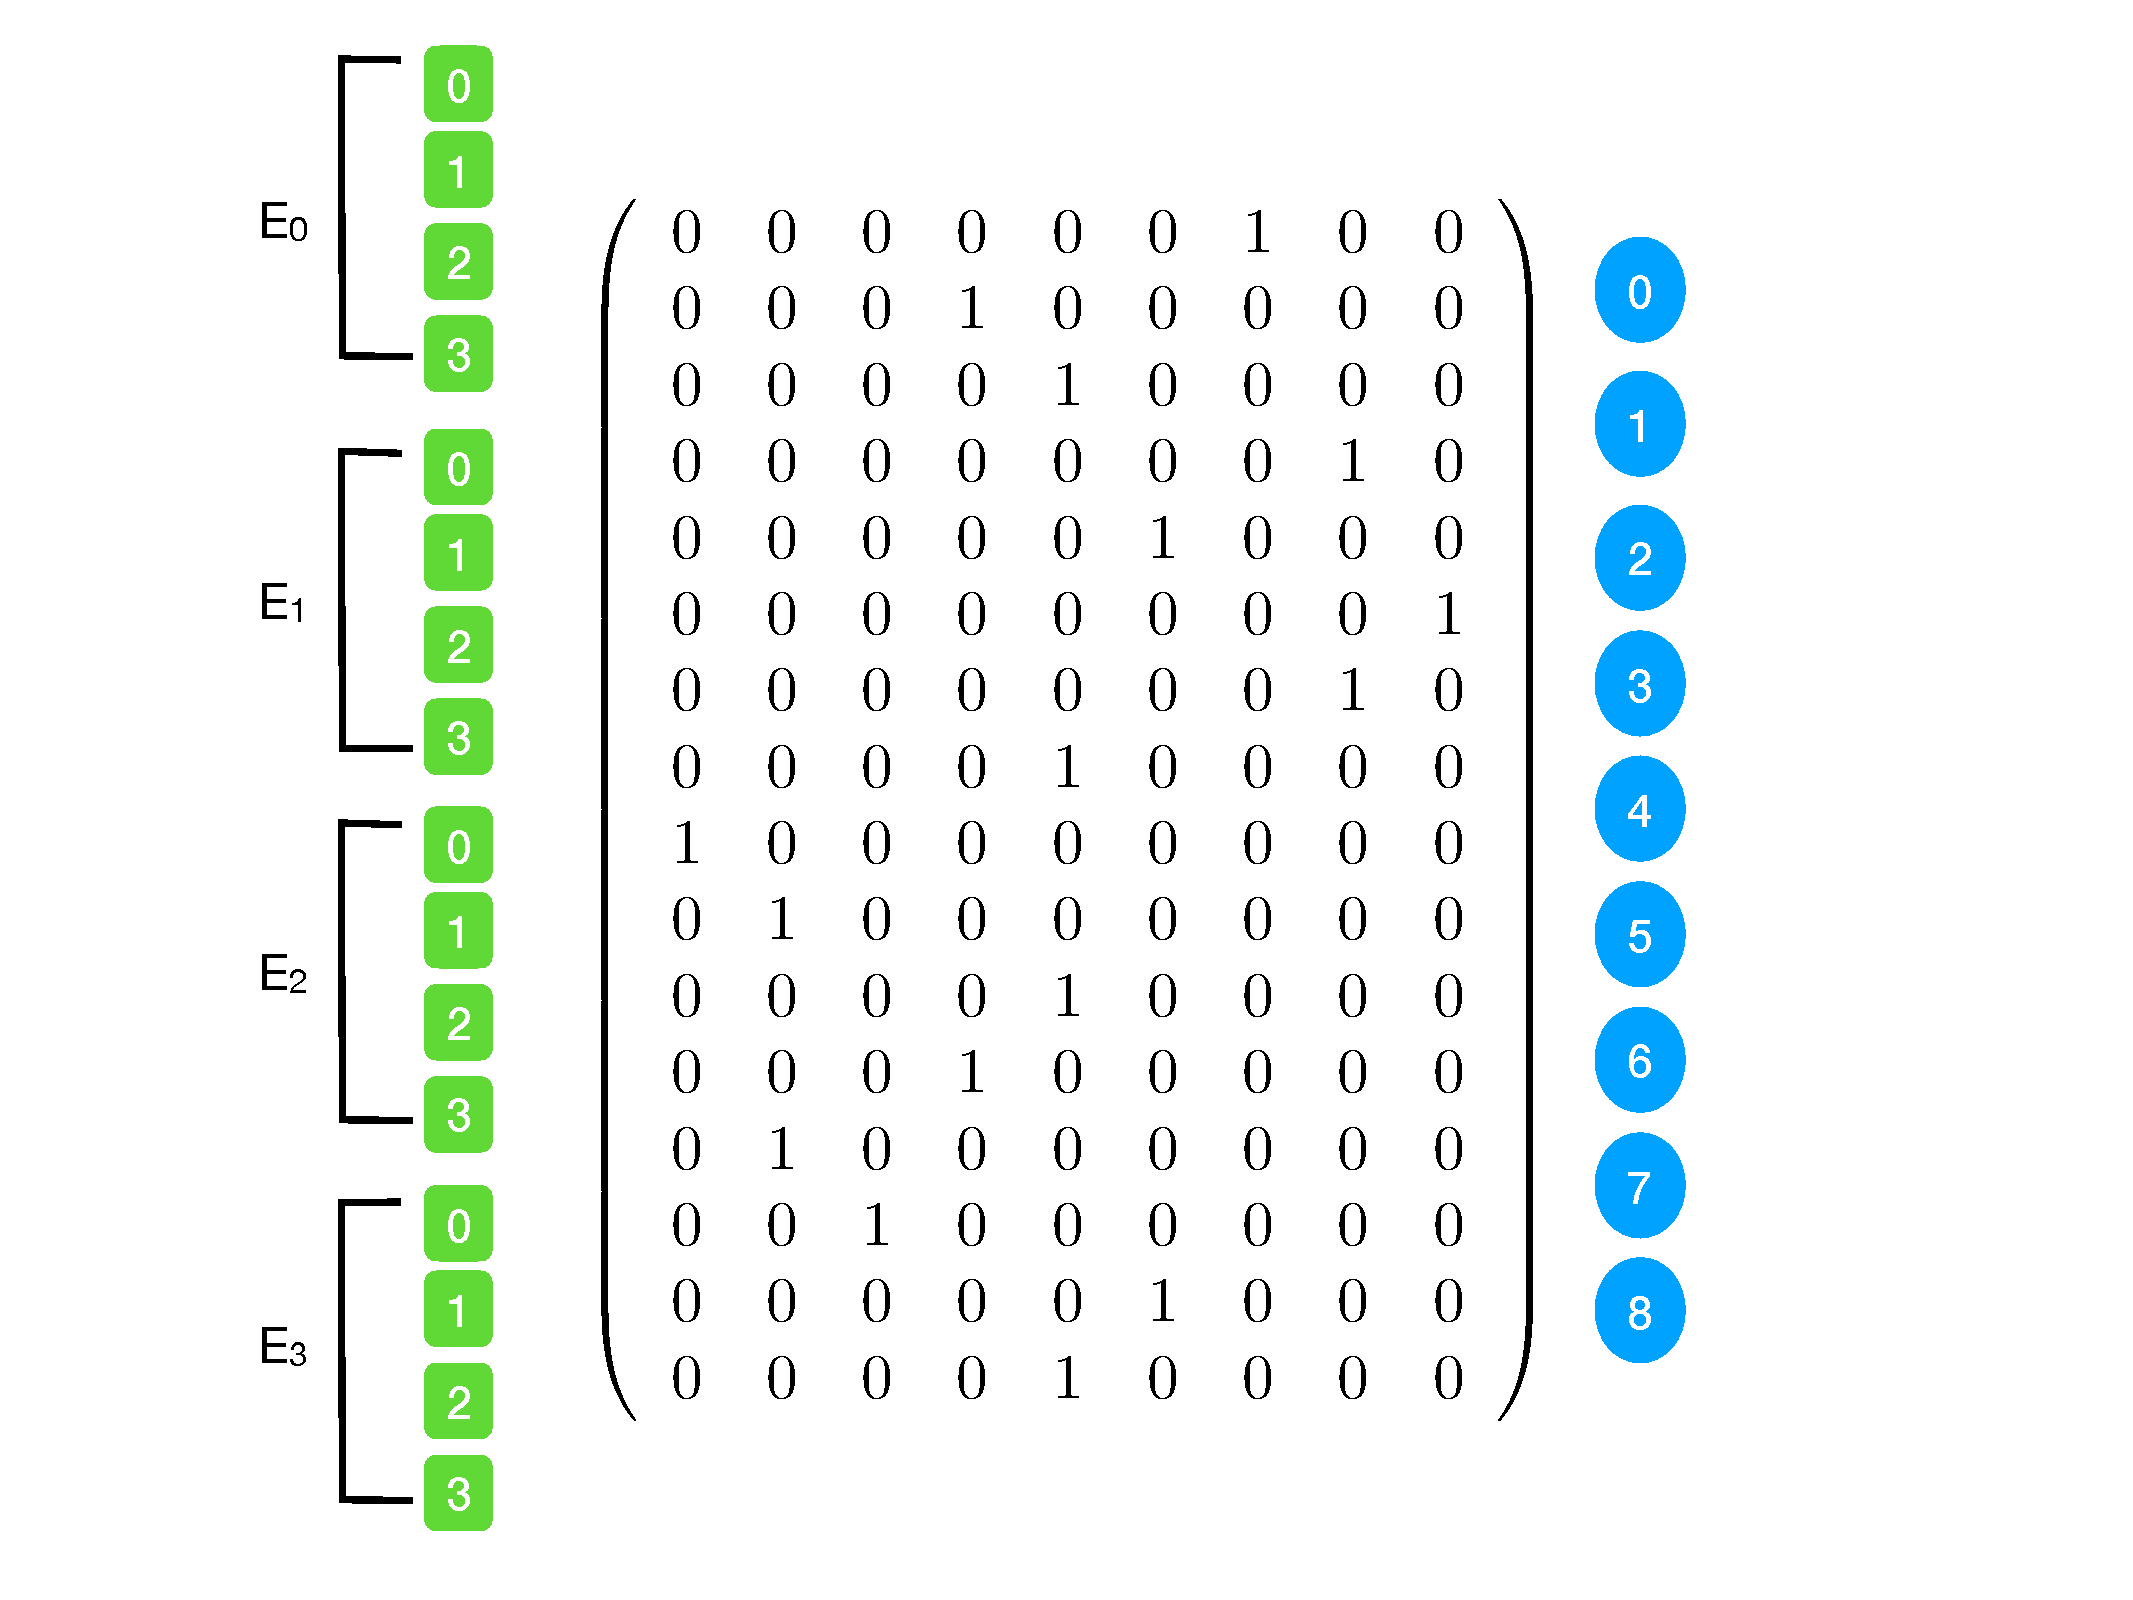
\includegraphics[width=4in]{img/Assembly2.pdf}
\caption{Diagram to help explain assembly.  UPDATE.}
\label{multiregions:assembly2}
\end{figure}


%
%
\section{The Fundamental Data Structures within MultiRegions}

As mentioned earlier, in almost all object-oriented languages (which includes $C++$), there exists the concepts of {\em class attributes} and {\em object attributes}.   For a summary of attributes and access patterns, please review Section \ref{sec:stdregions-datastructures}.
Within the MultiRegions directory of the library, there exists a class inheritance hierarchy designed to try to encourage re-use of core
algorithms (while simultaneously trying to minimize duplication of code).  We present this class hierarchy in Figure \ref{multiregions:multiregionstree}.


\begin{figure}[htb]
\centering
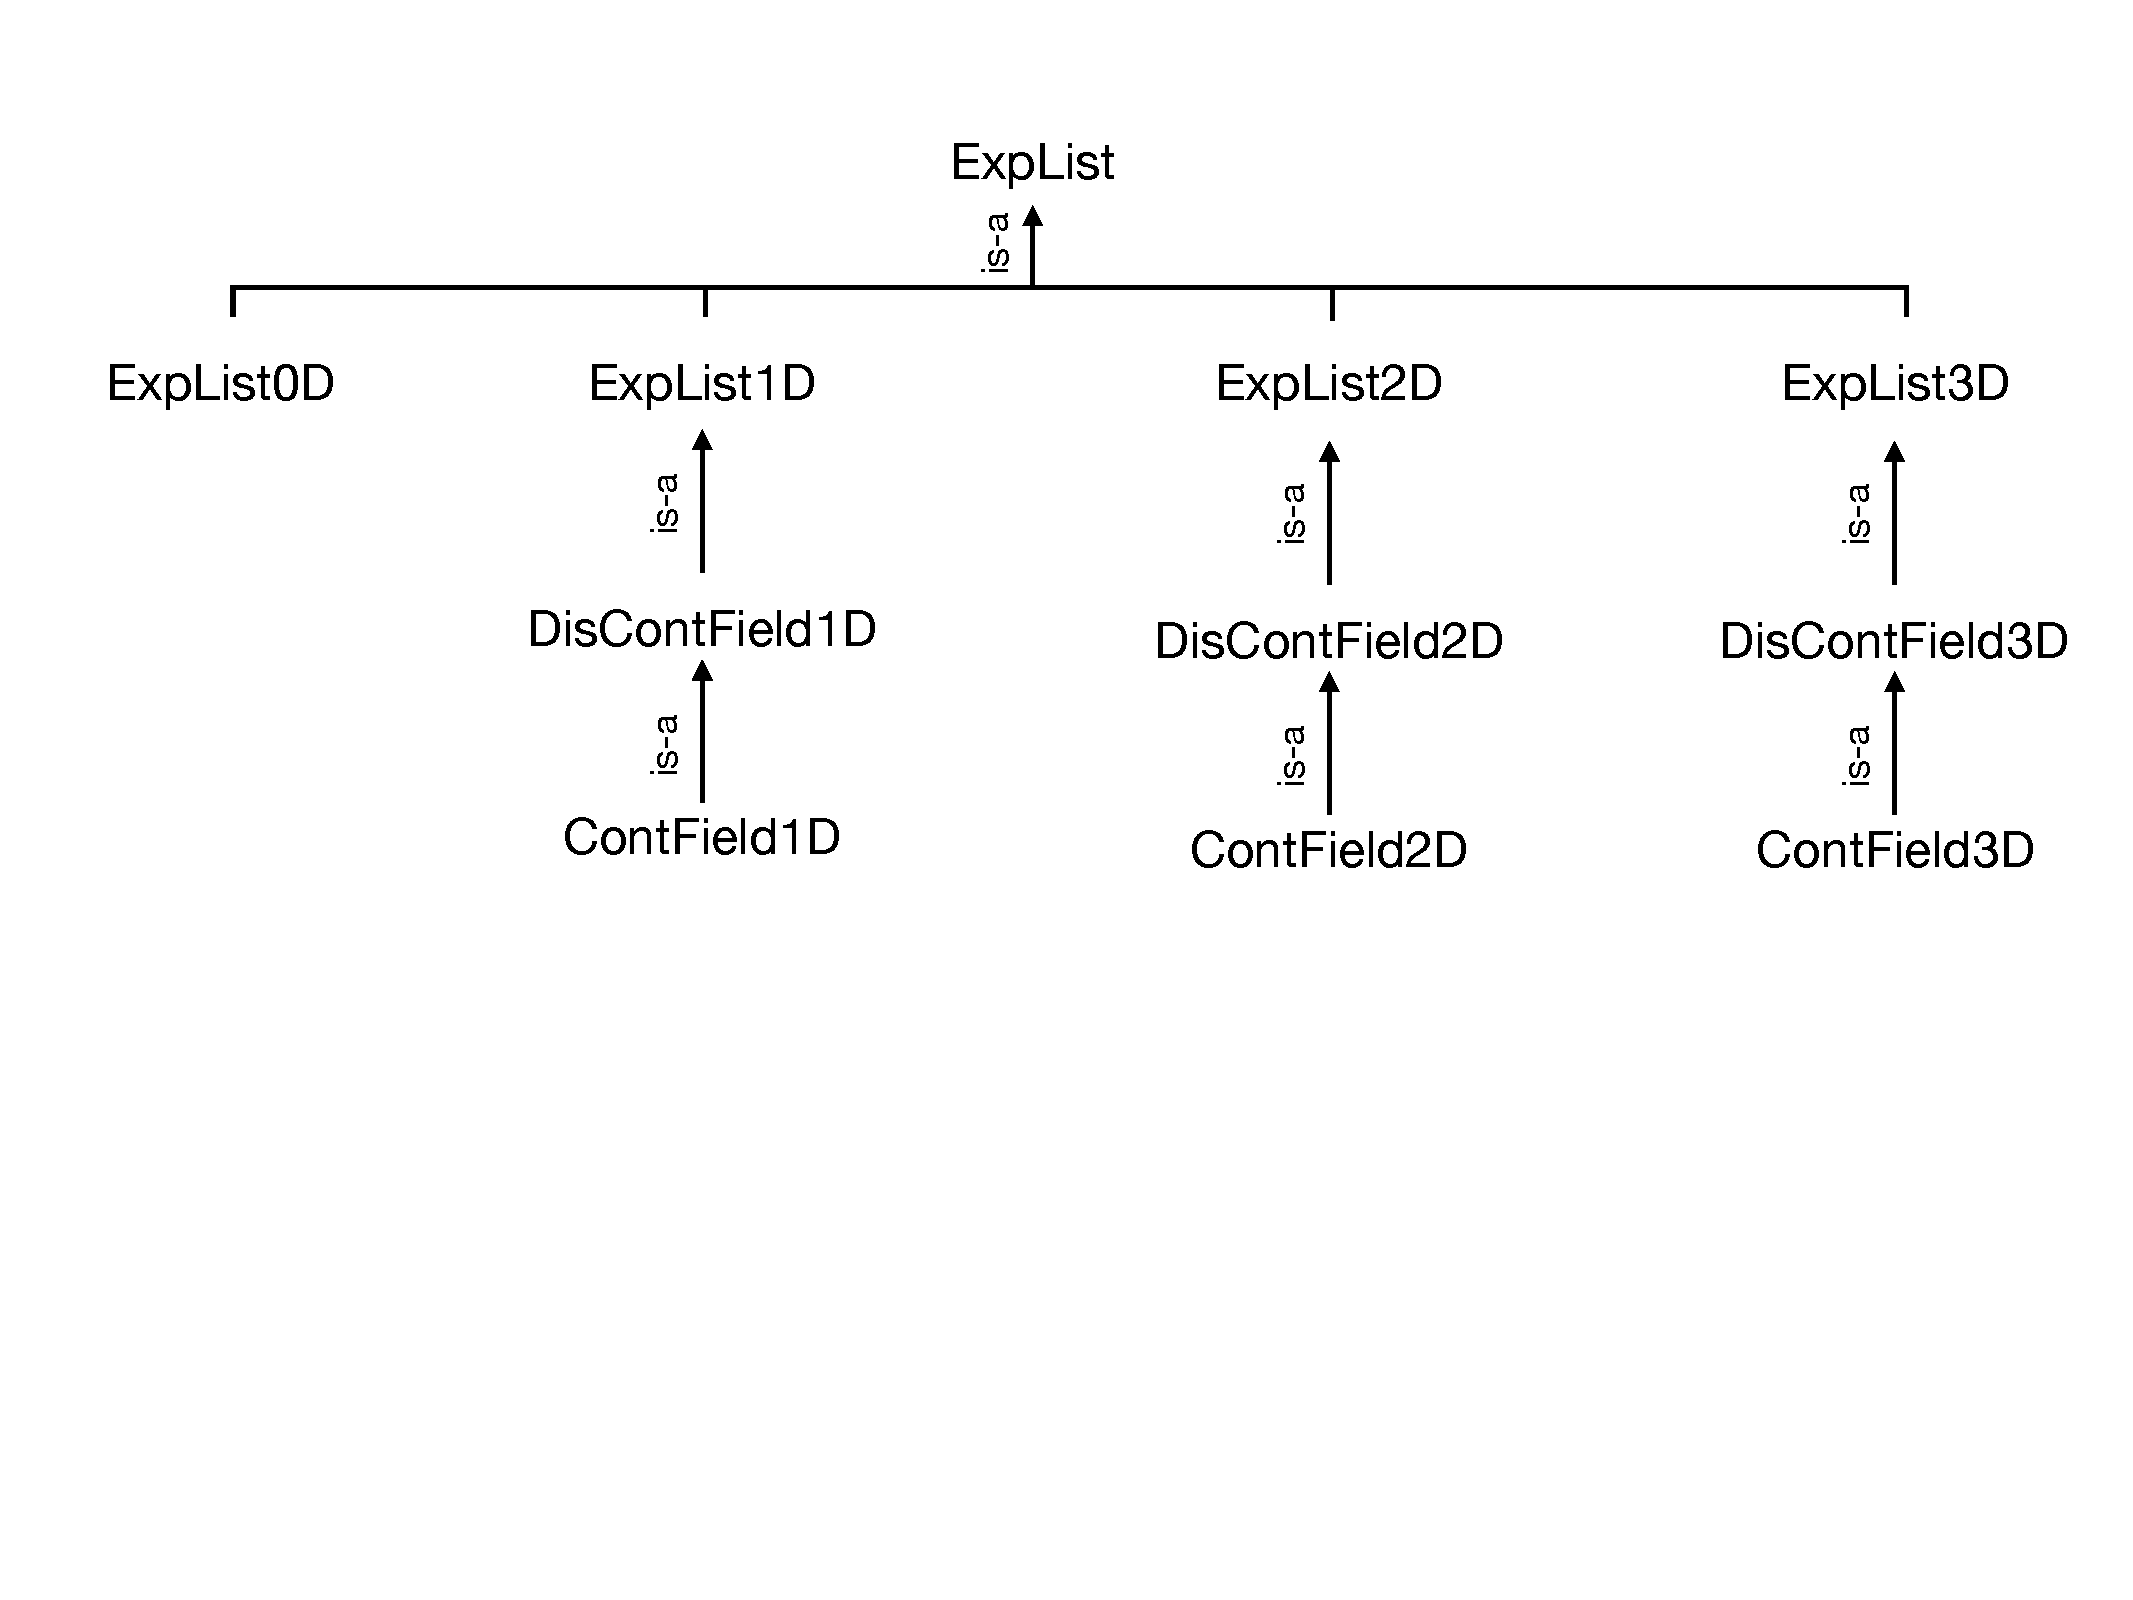
\includegraphics[width=6in]{img/multiregiontree.pdf}
\caption{Class hierarchy derived from ExpList, the base class of the MultiRegions Directory.}
\label{multiregions:multiregionstree}
\end{figure}

At its core, the items contained within MultiRegions are meant to represent sets of LocalRegions.  In the most abstract sense, an 
ExpList is merely a set of LocalRegion objects that may or may not have any relevance to each other.   We then, as we do in 
other parts of the library, specialize on the dimension of the objects these sets will contain.  At the subsequent levels of the
hierarchy, we now involve information about we want to treat a collection of elements when evaluating them as a {\em field}.  
We consider a {\em field} to be the representation of a function over a (sub--)domain.  A domain consists of a collection of elements
that are {\em connected} (that is, they form a contiguous region in space).   We think of the region of space as being tiled by elements
over which expansions are build.  If we consider a MultiRegion field to be a collection of these expansions with no constraints on their
continuity, we arrive at the DisContField family of class definitions (which vary by dimension).  For the currently available solvers within
{\nek}, this level of field is used for the solution of PDEs via the discontinuous Galerkin (dG) and Flux-Reconstruction (FR) methods.
If we consider a function as a collection of expansion in which we require continuity (in {\nek}, only $C^0$ continuity), then we employ
a further derived class called ContField (which again varies by dimension).  For the currently available solvers
within {\nek}, this level of field is used for the solution of PDEs via the continuous Galerkin (cG) method.
Since many of the operations at the continuous field level do not rely upon the continuity of the field, we have structured the
continuous MultiRegion object as with an {\em is-a} relationship with the DisContFields.

The various private, protected and public data members contained within MultiRegions are provided in the subsequent sections.


%%%%%%%%%%%%%%%%%%%%%%%%%%%%%%%%%%%%%%%%
\subsection{Variables at the Level of ExpList}

\paragraph{Private:}

\paragraph{Protected:}

\paragraph{Public:}


%%%%%%%%%%%%%%%%%%%%%%%%%%%%%%%%%%%%%%%%
\subsection{Variables at the Level of ExpList\$D for various Dimensions}

\paragraph{Private:}

\paragraph{Protected:}

\paragraph{Public:}


%%%%%%%%%%%%%%%%%%%%%%%%%%%%%%%%%%%%%%%%
\subsection{Variables at the Level of Discontinuous Field Expansions}

\paragraph{Private:}

\paragraph{Protected:}

\paragraph{Public:}


%%%%%%%%%%%%%%%%%%%%%%%%%%%%%%%%%%%%%%%%
\subsection{Variables at the Level of Continuous Field Expansions}

\paragraph{Private:}

\paragraph{Protected:}




%
%
\section{The Fundamental Algorithms within MultiRegions}

As stated in the introduction, this section of this guide is structured in question-answer form.  This is not meant to capture every possible
question asked of us on the {\nek} users list; however, this set of (ever-growing) questions are meant to capture the ``big ideas'' that developers 
want to know about how MultiRegions work and how they can be used.  

In this section, we will through question and answer format try to cover the following basic algorithmic concepts that are found within 
the MultiRegions part of the library:

\begin{itemize}
\item xx
\end{itemize}

With the big ideas in place, let us now start into our questions.

\paragraph{Question:}

%
\section{Preconditioners}
\label{sec:precon}

Most of the solvers in \nekpp, including the incompressible Navier-Stokes
equations, rely on the solution of a Helmholtz equation,
%
\begin{equation}
  \nabla^{2}u(\mathbf{x})+\lambda u(\mathbf{x})=f(\mathbf{x}),
  \label{eq:precon:helm}
\end{equation}
%
an elliptic boundary value problem, at every time-step, where $u$ is defined on
a domain $\Omega$ of $N_{\mathrm{el}}$ non-overlapping elements. In this
section, we outline the preconditioners which are implemented in \nekpp. Whilst
some of the preconditioners are generic, many are especially designed for the
\emph{modified} basis only.

\subsection{Mathematical formulation}

The standard spectral/$hp$ approach to discretise \eqref{eq:precon:helm} starts
with an expansion in terms of the elemental modes:
%
\begin{equation}
  u^{\delta}(\mathbf{x})=\sum_{n=0}^{N_{\mathrm{dof}}-1}\hat{u}_n
  \Phi_n(\mathbf{x})=\sum_{e=1}^{{N_{\mathrm{el}}}}
  \sum_{n=0}^{N^{e}_m-1}\hat{u}_n^e\phi_n^e(\mathbf{x})
  \label{eq:precon:disc}
\end{equation}
%
where $N_{\mathrm{el}}$ is the number of elements, $N^{e}_m$ is the number of
local expansion modes within the element $\Omega^e$, $\phi_n^e(\mathbf{x})$ is
the $n^{\mathrm{th}}$ local expansion mode within the element $\Omega^e$,
$\hat{u}_n^e$ is the $n^{\mathrm{th}}$ local expansion coefficient within the
element $\Omega^e$. Approximating our solution by~\eqref{eq:precon:disc}, we
adopt a Galerkin discretisation of equation~\eqref{eq:precon:helm} where for an
appropriate test space $V^\delta$ we find an approximate solution
$\mathbf{u}^{\delta} \in V^{\delta}$ such that
%
\[
\mathcal L \left({v, u}\right) = \int_{\Omega}\nabla v^{\delta} \cdot \nabla
u^{\delta} + \lambda v^{\delta} u^{\delta} d \mathbf{x} = \int_{\Omega}
v^{\delta} f d\mathbf{x} \quad \forall v^{\delta} \in V^{\delta}
\]
%
This can be formulated in matrix terms as
%
\[
\mathbf{H}\hat{\mathbf{u}} = \mathbf{f}
\]
%
where $\mathbf{H}$ represents the Helmholtz matrix, $\hat{\mathbf{u}}$ are the
unknown global coefficients and $\mathbf{f}$ the inner product the expansion
basis with the forcing function.

\subsubsection{$C^0$ formulation}

We first consider the $C^0$ (i.e. continuous Galerkin) formulation. The
spectral/$hp$ expansion basis is obtained by considering interior modes, which
have support in the interior of the element, separately from boundary modes
which are non-zero on the boundary of the element. We align the boundary modes
across the interface of the elements to obtain a continuous global solution. The
boundary modes can be further decomposed into vertex, edge and face modes,
defined as follows:

\begin{itemize}
  \item vertex modes have support on a single vertex and the three adjacent
  edges and faces as well as the interior of the element;
  \item edge modes have support on a single edge and two adjacent faces as well
  as the interior of the element; 
  \item face modes have support on a single face and the interior of the
  element.
\end{itemize}

When the discretisation is continuous, this strong coupling between vertices,
edges and faces leads to a matrix of high condition number $\kappa$. Our aim is
to reduce this condition number by applying specialised
preconditioners. Utilising the above mentioned decomposition, we can write the
matrix equation as:
%
\[
\left[\begin{array}{cc}
  \mathbf{H}_{bb} & \mathbf{H}_{bi}\\
  \mathbf{H}_{ib} & \mathbf{H}_{ii}
  \end{array}\right]
\left[ \begin{array}{c}
\hat{\mathbf{u}}_{b}\\
\hat{\mathbf{u}}_{i}\\
\end{array}\right] =
\left[ \begin{array}{c}
\hat{\mathbf{f}}_{b}\\
\hat{\mathbf{f}}_{i}\\
\end{array}\right]
\]
%
where the subscripts $b$ and $i$ denote the boundary and interior degrees of
freedom respectively. This system then can be statically condensed allowing us
to solve for the boundary and interior degrees of freedom in a decoupled
manor. The statically condensed matrix is given by
%
\[
\left[\begin{array}{cc}
  \mathbf{H}_{bb}-\mathbf{H}_{bi} \mathbf{H}_{ii}^{-1} \mathbf{H}_{ib} & 0\\
  \mathbf{H}_{ib} & \mathbf{H}_{ii}
  \end{array}\right]
\left[ \begin{array}{c}
\hat{\mathbf{u}}_{b}\\
\hat{\mathbf{u}}_{i}\\
\end{array}\right] =
\left[ \begin{array}{c}
\hat{\mathbf{f}}_{b}-\mathbf{H}_{bi} \mathbf{H}_{ii}^{-1}\hat{\mathbf{f}}_{i}\\
\hat{\mathbf{f}}_{i}\\
\end{array}\right]
\]
%
This is highly advantageous since by definition of our interior expansion this
vanishes on the boundary, and so $\mathbf{H}_{ii}$ is block diagonal and thus
can be easily inverted. The above sub-structuring has reduced our problem to
solving the boundary problem:
%
\[
\mathbf{S}_{1}\hat{\mathbf{u}} = \hat{\mathbf{f}}_{1}
\]
%
where
$\mathbf{S_{1}}=\mathbf{H}_{bb}-\mathbf{H}_{bi} \mathbf{H}_{ii}^{-1}
\mathbf{H}_{ib}$
and
$\hat{\mathbf{f}}_{1}=\hat{\mathbf{f}}_{b}-\mathbf{H}_{bi}
\mathbf{H}_{ii}^{-1}\hat{\mathbf{f}}_{i}$.
Although this new system typically has better convergence properties (i.e lower
$\kappa$), the system is still ill-conditioned, leading to a convergence rate of
the conjugate gradient (CG) routine that is prohibitively slow. For this reason
we need to precondition $\mathbf{S}_1$. To do this we solve an equivalent
system of the form:
%
\[
\mathbf{M}^{-1}\left(\mathbf{S}_{1} \hat{\mathbf{u}} - \hat{\mathbf{f}}_{1} \right) = 0
\]
%
where the preconditioning matrix $\mathbf{M}$ is such that
$\kappa\left(\mathbf{M}^{-1} \mathbf{S}_{1}\right)$ is less than
$\kappa\left(\mathbf{S}_{1}\right)$ and speeds up the convergence rate. Within
the conjugate gradient routine the same preconditioner $\mathbf{M}$ is applied
to the residual vector $\hat{\mathbf{r}}_{k+1}$ of the CG routine every
iteration:
%
\[
\hat{\mathbf{z}}_{k+1}=\mathbf{M}^{-1}\hat{\mathbf{r}}_{k+1}.
\]
%

\subsubsection{HDG formulation}

When utilising a hybridizable discontinuous Galerkin formulation, we perform a
static condensation approach but in a discontinuous framework, which for brevity
we omit here. However, we still obtain a matrix equation of the form
%
\[
\mathbf{\Lambda}\hat{\mathbf{u}} = \hat{\mathbf{f}}.
\]
%
where $\mathbf{\Lambda}$ represents an operator which projects the solution of
each face back onto the three-dimensional element or edge onto the
two-dimensional element. In this setting then, $\hat{\mathbf{f}}$ consists of
degrees of freedom for each egde (in 2D) or face (in 3D). The overall system
does not, therefore, results in a weaker coupling between degrees of freedom,
but at the expense of a larger matrix system.

\subsection{Preconditioners}

Within the \nekpp framework a number of preconditioners are available to speed
up the convergence rate of the conjugate gradient routine. The table below
summarises each method, the dimensions of elements which are supported, and also
the discretisation type support which can either be continuous (CG) or
discontinuous (hybridizable DG).

\begin{center}
  \begin{tabular}{lll}
    \toprule
    \textbf{Name}  & \textbf{Dimensions} & \textbf{Discretisations} \\
    \midrule
    \inltt{Null}                              & All  & All \\
    \inltt{Diagonal}                          & All  & All \\
    \inltt{FullLinearSpace}                   & 2/3D & CG  \\
    \inltt{LowEnergyBlock}                    & 3D   & CG  \\
    \inltt{Block}                             & 2/3D & All \\
    \midrule
    \inltt{FullLinearSpaceWithDiagonal}       & All  & CG  \\
    \inltt{FullLinearSpaceWithLowEnergyBlock} & 2/3D & CG  \\
    \inltt{FullLinearSpaceWithBlock}          & 2/3D & CG  \\
    \bottomrule
  \end{tabular}
\end{center}

The default is the \inltt{Diagonal} preconditioner. The above preconditioners
are specified through the \inltt{Preconditioner} option of the
\inltt{SOLVERINFO} section in the session file. For example, to enable
\inltt{FullLinearSpace} one can use:

\begin{lstlisting}[style=XMLStyle]
  <I PROPERTY="Preconditioner" VALUE="FullLinearSpace" />
\end{lstlisting}

Alternatively one can have more control over different preconditioners for each
solution field by using the \inltt{GlobalSysSoln} section. For more details,
consult the user guide. The following sections specify the details for each
method.

\subsubsection{Diagonal}

Diagonal (or Jacobi) preconditioning is amongst the simplest preconditioning
strategies. In this scheme one takes the global matrix $\mathbf{H} = (h_{ij})$
and computes the diagonal terms $h_{ii}$. The preconditioner is then formed as a
diagonal matrix $\mathbf{M}^{-1} = (h_{ii}^{-1})$.

\subsubsection{Linear space}

The linear space (or coarse space) of the matrix system is that containing
degrees of freedom corresponding only to the vertex modes in the high-order
system. Preconditioning of this space is achieved by forming the matrix
corresponding to the coarse space and inverting it, so that
%
\[
\mathbf{M}^{-1} = (\mathbf{S}^{-1}_{1})_{vv}
\]
%
Since the mesh associated with higher order methods is relatively coarse
compared with traditional finite element discretisations, the linear space can
usually be directly inverted without memory issues. However such a methodology
can be prohibitive on large parallel systems, due to a bottleneck in
communication.

In \nekpp the inversion of the linear space present is handled using the
$XX^{T}$ library. $XX^{T}$ is a parallel direct solver for problems of the form
$\mathbf{A}\hat{\mathbf{x}} = \hat{\mathbf{b}}$ based around a sparse
factorisation of the inverse of $\mathbf{A}$. To precondition utilising this
methodology the linear sub-space is gathered from the expansion and the
preconditioned residual within the CG routine is determined by solving
%
\[
(\mathbf{S}_{1})_{vv}\hat{\mathbf{z}}=\hat{\mathbf{r}}
\]
%
The preconditioned residual $\hat{\mathbf{z}}$ is then scattered back to the
respective location in the global degrees of freedom.

\subsubsection{Block}

Block preconditioning of the $C^0$ continuous system is defined by the
following:
%
\[
\mathbf{M}^{-1}=\left[ \begin{array}{ccc}
(\mathbf{S}^{-1}_{1})_{vv} & 0 & 0 \\
0 & (\mathbf{S}^{-1}_{1})_{eb} & 0\\
0 & 0 & (\mathbf{S}^{-1}_{1})_{ef}\\
 \end{array} \right]
\]
%
where $\mathrm{diag}[(\mathbf{S}_{1})_{vv}]$ is the diagonal of the vertex
modes, $(\mathbf{S}_{1})_{eb}$ and $(\mathbf{S}_{1})_{fb}$ are block diagonal
matrices corresponding to coupling of an edge (or face) with itself i.e ignoring
the coupling to other edges and faces. This preconditioner is best suited for
two dimensional problems.

In the HDG system, we take the block corresponding to each face and invert
it. Each of these inverse blocks then forms one of the diagonal components of
the block matrix $\mathbf{M}^{-1}$.

\subsection{Low energy}

Low energy basis preconditioning follows the methodology proposed by Sherwin \&
Casarin. In this method a new basis is numerically constructed from the original
basis which allows the Schur complement matrix to be preconditioned using a
block preconditioner. The method is outlined briefly in the following.

Elementally the local approximation $\mathbf{u}^{\delta}$ can be expressed as
different expansions lying in the same discrete space $V^{\delta}$
%
\[
\mathbf{u}^{\delta}(\mathbf{x})=\sum_{i}^{\dim(V^{\delta})}\hat{u}_{1i}\phi_{1i}(x)
= \sum_{i}^{\dim(V^{\delta})}\hat{u}_{2i}\phi_{2j}(x)
\]
%
Since both expansions lie in the same space it's possible to express one basis
in terms of the other via a transformation, i.e.
%
\[
\phi_{2}=\mathbf{C}\phi_{1} \implies \hat{\mathbf{u}}_{1}=C^{T}\hat{\mathbf{u}}_{2}
\]
%
Applying this to the Helmholtz operator it is possible to show that,
%
\[
\mathbf{H}_{2}=\mathbf{C}\mathbf{H}_{1}\mathbf{C}^{T}
\]
%
For sub-structured matrices ($\mathbf{S}$) the transformation matrix
($\mathbf{C}$) becomes:
%
\[
\mathbf{C}=\left[ \begin{array}{cc}
\mathbf{R} & 0\\
0 & \mathbf{I}
 \end{array} \right]
\]
%
Hence the transformation in terms of the Schur complement matrices is:
%
\[
\mathbf{S}_{2}=\mathbf{R}\mathbf{S}_{1}\mathbf{R}^{T}
\]
%
Typically the choice of expansion basis $\phi_{1}$ can lead to a Helmholtz
matrix that has undesirable properties i.e poor condition number. By choosing a
suitable transformation matrix $\mathbf{C}$ it is possible to construct a new
basis, numerically, that is amenable to block diagonal preconditioning.
%
\[
\mathbf{S}_{1}=\left[ \begin{array}{ccc}
\mathbf{S}_{vv} & \mathbf{S}_{ve} & \mathbf{S}_{vf}\\
\mathbf{S}^{T}_{ve}& \mathbf{S}_{ee} & \mathbf{S}_{ef} \\
\mathbf{S}^{T}_{vf} & \mathbf{S}^{T}_{ef} & \mathbf{S}_{ff} \end{array} \right] =\left[ \begin{array}{cc}
\mathbf{S}_{vv} & \mathbf{S}_{v,ef} \\
\mathbf{S}^{T}_{v,ef} & \mathbf{S}_{ef,ef} \end{array} \right]
\]
%
Applying the transformation
$\mathbf{S}_{2}=\mathbf{R} \mathbf{S}_{1} \mathbf{R}^{T}$ leads to the following
matrix
%
\[
\mathbf{S}_{2}=\left[ \begin{array}{cc}
\mathbf{S}_{vv}+\mathbf{R}_{v}\mathbf{S}^{T}_{v,ef}+\mathbf{S}_{v,ef}\mathbf{R}^{T}_{v}+\mathbf{R}_{v}\mathbf{S}_{ef,ef}\mathbf{R}^{T}_{v} & [\mathbf{S}_{v,ef}+\mathbf{R}_{v}\mathbf{S}_{ef,ef}]\mathbf{A}^{T} \\
\mathbf{A}[\mathbf{S}^{T}_{v,ef}+\mathbf{S}_{ef,ef}\mathbf{R}^{T}_{v}] & \mathbf{A}\mathbf{S}_{ef,ef}\mathbf{A}^{T} \end{array} \right]
\]
%
where $\mathbf{A}\mathbf{S}_{ef,ef}\mathbf{A}^{T}$ is given by
%
\[
\mathbf{A}\mathbf{S}_{ef,ef}\mathbf{A}^{T}=\left[ \begin{array}{cc}
\mathbf{S}_{ee}+\mathbf{R}_{ef}\mathbf{S}^{T}_{ef}+\mathbf{S}_{ef}\mathbf{R}^{T}_{ef}+\mathbf{R}_{ef}\mathbf{S}_{ff}\mathbf{R}^{T}_{ef} & \mathbf{S}_{ef}+\mathbf{R}_{ef}\mathbf{S}_{ff}\\
\mathbf{S}^{T}_{ef}+\mathbf{S}_{ff}\mathbf{R}^{T}_{ef} & \mathbf{S}_{ff}
 \end{array} \right]
\]
%
To orthogonalise the vertex-edge and vertex-face modes, it can be seen from the
above that
%
\[
\mathbf{R}^{T}_{ef}=-\mathbf{S}^{-1}_{ff}\mathbf{S}^{T}_{ef}
\]
%
and for the edge-face modes:
%
\[
\mathbf{R}^{T}_{v}=-\mathbf{S}^{-1}_{ef,ef}\mathbf{S}^{T}_{v,ef}
\]
%
Here it is important to consider the form of the expansion basis since the
presence of $\mathbf{S}^{-1}_{ff}$ will lead to a new basis which has support on
all other faces; this is problematic when creating a $C^{0}$ continuous global
basis.  To circumvent this problem when forming the new basis, the decoupling is
only performed between a specific edge and the two adjacent faces in a symmetric
standard region. Since the decoupling is performed in a rotationally symmetric
standard region the basis does not take into account the Jacobian mapping
between the local element and global coordinates, hence the final expansion will
not be completely orthogonal.

The low energy basis creates a Schur complement matrix that although it is not
completely orthogonal can be spectrally approximated by its block diagonal
contribution. The final form of the preconditioner is:
%
\[
\mathbf{M}^{-1}=\left[ \begin{array}{ccc}
\mathrm{diag}[(\mathbf{S}_{2})_{vv}] & 0 & 0 \\
0 & (\mathbf{S}_{2})_{eb} & 0\\
0 & 0 & (\mathbf{S}_{2})_{fb}\\
 \end{array} \right]^{-1}
\]
%
where $\mathrm{diag}[(\mathbf{S}_{2})_{vv}]$ is the diagonal of the vertex
modes, $(\mathbf{S}_{2})_{eb}$ and $(\mathbf{S}_{2})_{fb}$ are block diagonal
matrices corresponding to coupling of an edge (or face) with itself i.e ignoring
the coupling to other edges and faces.




%%%%%%%%%%%%%%%%%%%%%%%%%%%%%%%
\chapter{Inside the Library: GlobalMapping}
\label{chapter:globalmapping} 

In this chapter, we walk the reader through the different components
of the GlobalMapping Directory.  We begin with a discussion of the
mathematical fundamentals, for which we use research article by
Cantwell et al. \cite{CantwellYKPS14} and the book \cite{Ar89} as our
principle references.  We then provide the reader with an overview of
the primary data structures introduced within the GlobalMapping
Directory (often done through C++ objects), and then present the major
algorithms -- expressed as either object methods or functions --
employed over these data structures.

%
\section{The Fundamentals Behind GlobalMapping}

Based upon the appendix in \cite{CantwellYKPS14}, we 
outline a rigorous derivation of the Laplace-Beltrami operator.
We use the convention that
indices appearing once in the upper position and once in the lower position are
considered dummy indices and are implicitly summed over their range, while
non-repeated indices are considered free to take any value. Derivatives are also
denoted using the lower-index comma notation, for example $g_{ij,k}$.
{\em Covariant} vectors such as the gradient are those which, under a change of
coordinate system, change under the same transformation in order to maintain
coordinate system invariance. In contrast, {\em contravariant} vectors, such as
velocity, should remain fixed under a coordinate transformation requiring that
their components change under the inverse of the transformation to maintain
invariance.
With this in mind, we now construct the fundamental differential operators we
require for a 2-dimensional manifold embedded in a 3-dimensional space.
In order to express these operators in curvilinear coordinates we start by
assuming that we have a smooth surface parametrization given by
\begin{align*}
	\mathbf{x}(\xi^1,\xi^2):=(x^1(\xi^1,\xi^2),x^2(\xi^1,\xi^2),x^3(\xi^1,\xi^2)).
%    \label{A:parametrization}
\end{align*}
Next we will define the Jacobian of $\mathbf{x}$ as the tensor
\begin{align*}
        J_i^j = \frac{\partial x^j}{\partial \xi^i}
%    \label{A:jacobian}
\end{align*}
where $J_i^j$ can be viewed as a covariant surface vector (by fixing the upper 
index) or as a contravariant space vector (by fixing the lower index). The
surface metric tensor $g_{ij}$ can be defined in terms of the $J_i^j$ as
\begin{align}
    g_{ij} = \sum_{k=1}^3 J_i^k J_j^k.
    \label{A:metric_tensor}
\end{align}
which can be considered to transform a contravariant quantity to a covariant 
quantity. Similarly the conjugate tensor $g^{ij}$, which does the reverse 
transformation, is given by
\begin{align}
    g^{11} = g_{22}/g,\quad g^{12} = g^{21} = - g_{12}/g,\quad g^{22} = g_{11}/g,
    \label{A:conj_tensor}
\end{align}
where $g$ is the determinant of $g_{ij}$. The metric tensor and its conjugate
satisfy the condition
\begin{align*}
    \delta_i^j = g_{ik}g^{jk} = 
    \begin{cases}
        1,\; &\mbox{if } i = j,\\
        0,\; &\mbox{if } i\ne j.
    \end{cases}
\end{align*}
% %
To construct the divergence operator we will also need the derivative of 
$g$ with respect to components of the metric, $g_{ij}$. We know that $\mathbf{g}$ 
is invertible and from linear algebra we have that the inverse of the metric 
\eqref{A:conj_tensor} satisfies 
$\mathbf{g}^{-1} = \frac{1}{g}\tilde{\mathbf{g}}^{\top}$, where $\mathbf{\tilde{g}}$ is the
cofactor matrix of $\mathbf{g}$. Therefore $\mathbf{\tilde{g}}^{\top} = g\BM{g}^{-1}$, 
or in components $\tilde{g}^{ij} = g(\BM{g}^{-1})_{ji}$. Using Jacobi's formula 
for the derivative of a matrix determinant with respect its entries, and since 
$\mathbf{g}$ is invertible, the derivative of the metric determinant is
\begin{align}
    \frac{\partial g}{\partial g_{ij}} = \mathrm{tr}\left(\tilde{\mathbf{g}}^{\top}\frac{\partial \mathbf{g}}{\partial g_{ij}}\right)
        = \tilde{g}^{ij} = g(\BM{g}^{-1})_{ji} = gg^{ij}.
\label{A:g_deriv}
\end{align}


\subsection{Divergence operator}
The partial derivative of a tensor with respect to a manifold coordinate system
is itself not a tensor. In order to obtain a tensor, one has to use 
\emph{covariant} derivative, defined below.
% %
The covariant derivative of a contravariant vector is given by
\begin{align}
    \nabla_k a^i = a^i_{,k} + a^j \Gamma_{jk}^i.
    \label{A:cov_diff}
\end{align}
where $\Gamma_{jk}^i$ are \emph{Christoffel Symbols of the second kind}.
% %
The \emph{Christoffel symbols of the first kind} are defined by
\begin{align*}
    \Gamma_{ijk} = \frac{1}{2}\left[g_{kj,i} + g_{ik,j} - g_{ij,k}\right].
%    \label{A:CS1}
\end{align*}
Here we note that $\Gamma_{ijk}$ is symmetric in the first two indices. To 
obtain the Christoffel symbols of the second kind we formally raise the 
last index using the conjugate tensor,
\begin{align}
    \Gamma_{ij}^l = \Gamma_{ijk}g^{kl}
    \label{A:CS2}
\end{align}
which retains the symmetry in the lower two indices. We can now express the
derivatives of the metric tensor in terms of the Christoffel symbols as
\begin{align*}
    g_{ij,k} = \Gamma_{ikj} + \Gamma_{jki} 
             = g_{lj}\Gamma_{ik}^l + g_{li}\Gamma_{jk}^l.
%    \label{A:metric_through_CS}
\end{align*}

We now define the divergence operator on the manifold,
$\nabla\cdot \mathbf{X} = \nabla_k X^k$. Consider first the derivative of the 
determinant of the metric tensor $g$ with respect to 
the components of some local coordinates system $\xi^1,\xi^2$. We apply the 
chain rule, making use of the derivative of the metric tensor with respect to 
components of the metric \eqref{A:g_deriv} and the relationship \eqref{A:CS2}, 
to get
\begin{align}
    \frac{\partial g}{\partial \xi^k} = \frac{\partial g}{\partial g_{ij}}\frac{\partial g_{ij}}{\partial \xi^k} = 
    gg^{ij}g_{ij,k} = gg^{ij}(\Gamma_{ikj} + \Gamma_{jki}) = g(\Gamma_{ik}^i + \Gamma_{jk}^j) = 2g\Gamma_{ik}^i.
    \label{A:g_deriv2}
\end{align}
We can therefore express the Christoffel symbol $\Gamma_{ik}^i$ in terms of this
derivative as
\begin{align}
    \Gamma_{ik}^i = \frac{1}{2g}\frac{\partial g}{\partial \xi^k} = \frac{1}{\sqrt{g}}\frac{\partial\sqrt{g}}{\partial \xi^k}.
    \label{A:G_ik^i}
\end{align}
Finally, by substituting for $\Gamma_{ik}^i$ in the expression for the 
divergence operator
\begin{align*}
 \nabla_k X^k &= X^k_{,k} + X^i\Gamma_{ki}^k \\ 
              &= X^k_{,k} + X^k\Gamma_{ik}^i \\
              &= X^k_{,k} + X^k\frac{1}{\sqrt{g}}(\sqrt{g})_{,k}
\end{align*}
we can deduce a formula for divergence of a contravariant vector as
\begin{align}
\nabla\cdot \mathbf{X} = \nabla_k X^k = \frac{\left(X^k\sqrt{g}\right)_{,k}}{\sqrt{g}}
\label{A:div}
\end{align}


\subsection{Laplacian operator} 
The covariant derivative (gradient) of a scalar on the manifold is identical to
the partial derivative, $\nabla_k \phi = \phi_{,k}$.
To derive the Laplacian operator we need the contravariant form of the covariant
gradient above which can be found by raising the index using the metric tensor,
giving
\begin{align}
    \nabla^k \phi = g^{kj}\phi_{,j},
    \label{A:covar-div}
\end{align}
and substituting \eqref{A:covar-div} for $X^k$ in \eqref{A:div} to get the Laplacian operator
on the manifold as
\begin{align}
    \Delta_M\phi = \frac{1}{\sqrt{g}}\left(\sqrt{g}g^{ij}\phi_{,j}\right)_{,i}.
    \label{A:surf_lapl}
\end{align}


\subsection{Anisotropic diffusion}
 We now extend the above operator to allow for anisotropic diffusion in the domain by deriving an expression for the surface conductivity from the ambient conductivity. The gradient of a surface function scaled by the ambient conductivity tensor $\tilde{\nabla}^p$ is given by
 \begin{align}
     \tilde{\nabla}^p f = g^{mp} J^l_m \sigma_{kl} J^k_j g^{ij} \frac{\partial f}{\partial x^i}.
 \end{align}
 The surface gradient is mapped to the ambient space through the Jacobian $J^k_j$, scaled by the ambient conductivity, and mapped back to the surface through $J^l_m$. The anisotropic Laplacian operator is given by
 \begin{align}
     \tilde{\nabla}^2 f = \nabla_k \tilde{\nabla}^k f = \nabla_k \tilde{\sigma}^{ij} \nabla_j f
 \end{align}
 Therefore the surface conductivity tensor can be computed using the Jacobian tensor and the inverse metric as
 \begin{align}
     \mathbf{\tilde{\sigma}} = \mathbf{g^{-1}J\sigma J^{\top} g^{-1}}.
 \end{align}


\subsection{Anisotropic Laplacian operator}
\label{s:anisotropic}
Anisotropic diffusion is important in many applications. In the ambient 
Euclidean space, this can be represented by a diffusivity tensor $\mathbf{\sigma}$ 
in the Laplacian operator as
\begin{align*}
\Delta_M = \nabla \cdot \mathbf{\sigma} \nabla.
\end{align*}
On our manifold, we seek the generalisation of \ref{A:surf_lapl}, in the form
\begin{align*}
\tilde{\Delta}_M \phi = \nabla_j \tilde{\sigma}_i^j \nabla^i \phi.
\end{align*}
where the $\tilde{\sigma}_i^j$ are entries in the surface diffusivity.
% %
For a contravariant surface vector $a^j$ we can find the associated
space vector $A^i$ as $A^i = J^i_j a^j$. Similarly if $A_i$ is a covariant space vector, then $a_j=J^i_j A_i$ is a covariant surface vector. 
% %
Using these we can construct the anisotropic
diffusivity tensor $\tilde{\mathbf{\sigma}}$ on the manifold by constraining the ambient diffusivity tensor $\mathbf{\sigma}$ to the surface. The contravariant surface gradient $\nabla^i \phi$ is mapped to the corresponding space vector, which lies in the tangent plane to the surface. This is scaled by the ambient diffusivity and then projected back to a covariant surface vector. Finally, we use the conjugate metric to convert back to a contravariant form. The resulting surface Laplacian is 
\begin{align*}
    \tilde{\Delta}_M \phi = \nabla_m g^{lm}J^k_l\sigma_{jk}J^j_i \nabla^i \phi.
\end{align*}
Following on from this we deduce that
\begin{align*}
    \tilde{\sigma}_i^j = g^{jm} J^l_m \sigma_{lk} J^k_i.
\end{align*}
It can be seen that in the case of isotropic diffusion that $\tilde{\sigma}_i^j = \delta^i_j \Leftrightarrow \mathbf{\sigma} = \mathbf{I}$,
\begin{align*}
    \tilde{\sigma}_i^j = g^{im} J^k_m \sigma_{lk} J^l_j = g^{im} J^k_m J^k_j = g^{im} g_{mj} = \delta^i_j.
\end{align*}

%
%
\section{The Fundamental Data Structures within GlobalMapping}
%
%
\section{The Fundamental Algorithms within GlobalMapping}


%%%%%%%%%%%%%%%%%%%%%%%%%%%%%%%
\chapter{Inside the Library: FieldUtils}

In this chapter, we walk the reader through the different components of the FieldUtils Directory.
We begin with a discussion of the mathematical fundamentals, for which we use the book
by Karniadakis and Sherwin \cite{KaSh05} as our principle reference.  We then provide
the reader with an overview of the primary data structures introduced within the
FieldUtils Directory (often done through C++ objects), and then present the major 
algorithms -- expressed as either object methods or functions -- employed over these data structures.  

%
\section{The Fundamentals Behind FieldUtils}
%
%
\section{The Fundamental Data Structures within FieldUtils}
%
%
\section{The Fundamental Algorithms within FieldUtils}


%%%%%%%%%%%%%%%%%%%%%%%%%%%%%%%
\chapter{Inside the Library: SolverUtils}

In this chapter, we walk the reader through the different components of the SolverUtils Directory.
We begin with a discussion of the mathematical fundamentals, for which we use the book
by Karniadakis and Sherwin \cite{KaSh05} as our principle reference.  We then provide
the reader with an overview of the primary data structures introduced within the
SolverUtils Directory (often done through C++ objects), and then present the major 
algorithms -- expressed as either object methods or functions -- employed over these data structures.  

%
\section{The Fundamentals Behind SolverUtils}
%
%
\section{The Fundamental Data Structures within SolverUtils}
%
%
\section{The Fundamental Algorithms within SolverUtils}
\subsection{Filters}
\subsubsection{Lagrangian Points Tracking}
In the filter \texttt{FilterLagrangianPoints}, Lagrangian points can be tracked in parallel. In this filter, Points are stored in two copies. One copy is the stationary points, which are fixed in the thread. Another copy is the mobile points, which can move based on the mesh partition. When evaluating the physics values on the mobile points, we first search the local mesh partition. For the points that are not found in the local partition, their information is packed into a global array and synced for all thread. A global search is performed. Once the thread whose mesh partition contains some unfound mobile points,  these points in the mobile copy are moved to the corresponding thread. After evaluation the physics values on the mobile points, the data are sent back to thread which contains the corresponding stationary points. The design detail of this filter is shown in figure~\ref{fig:LagrangianTrack}.
\begin{figure}[htp]
    \centering
    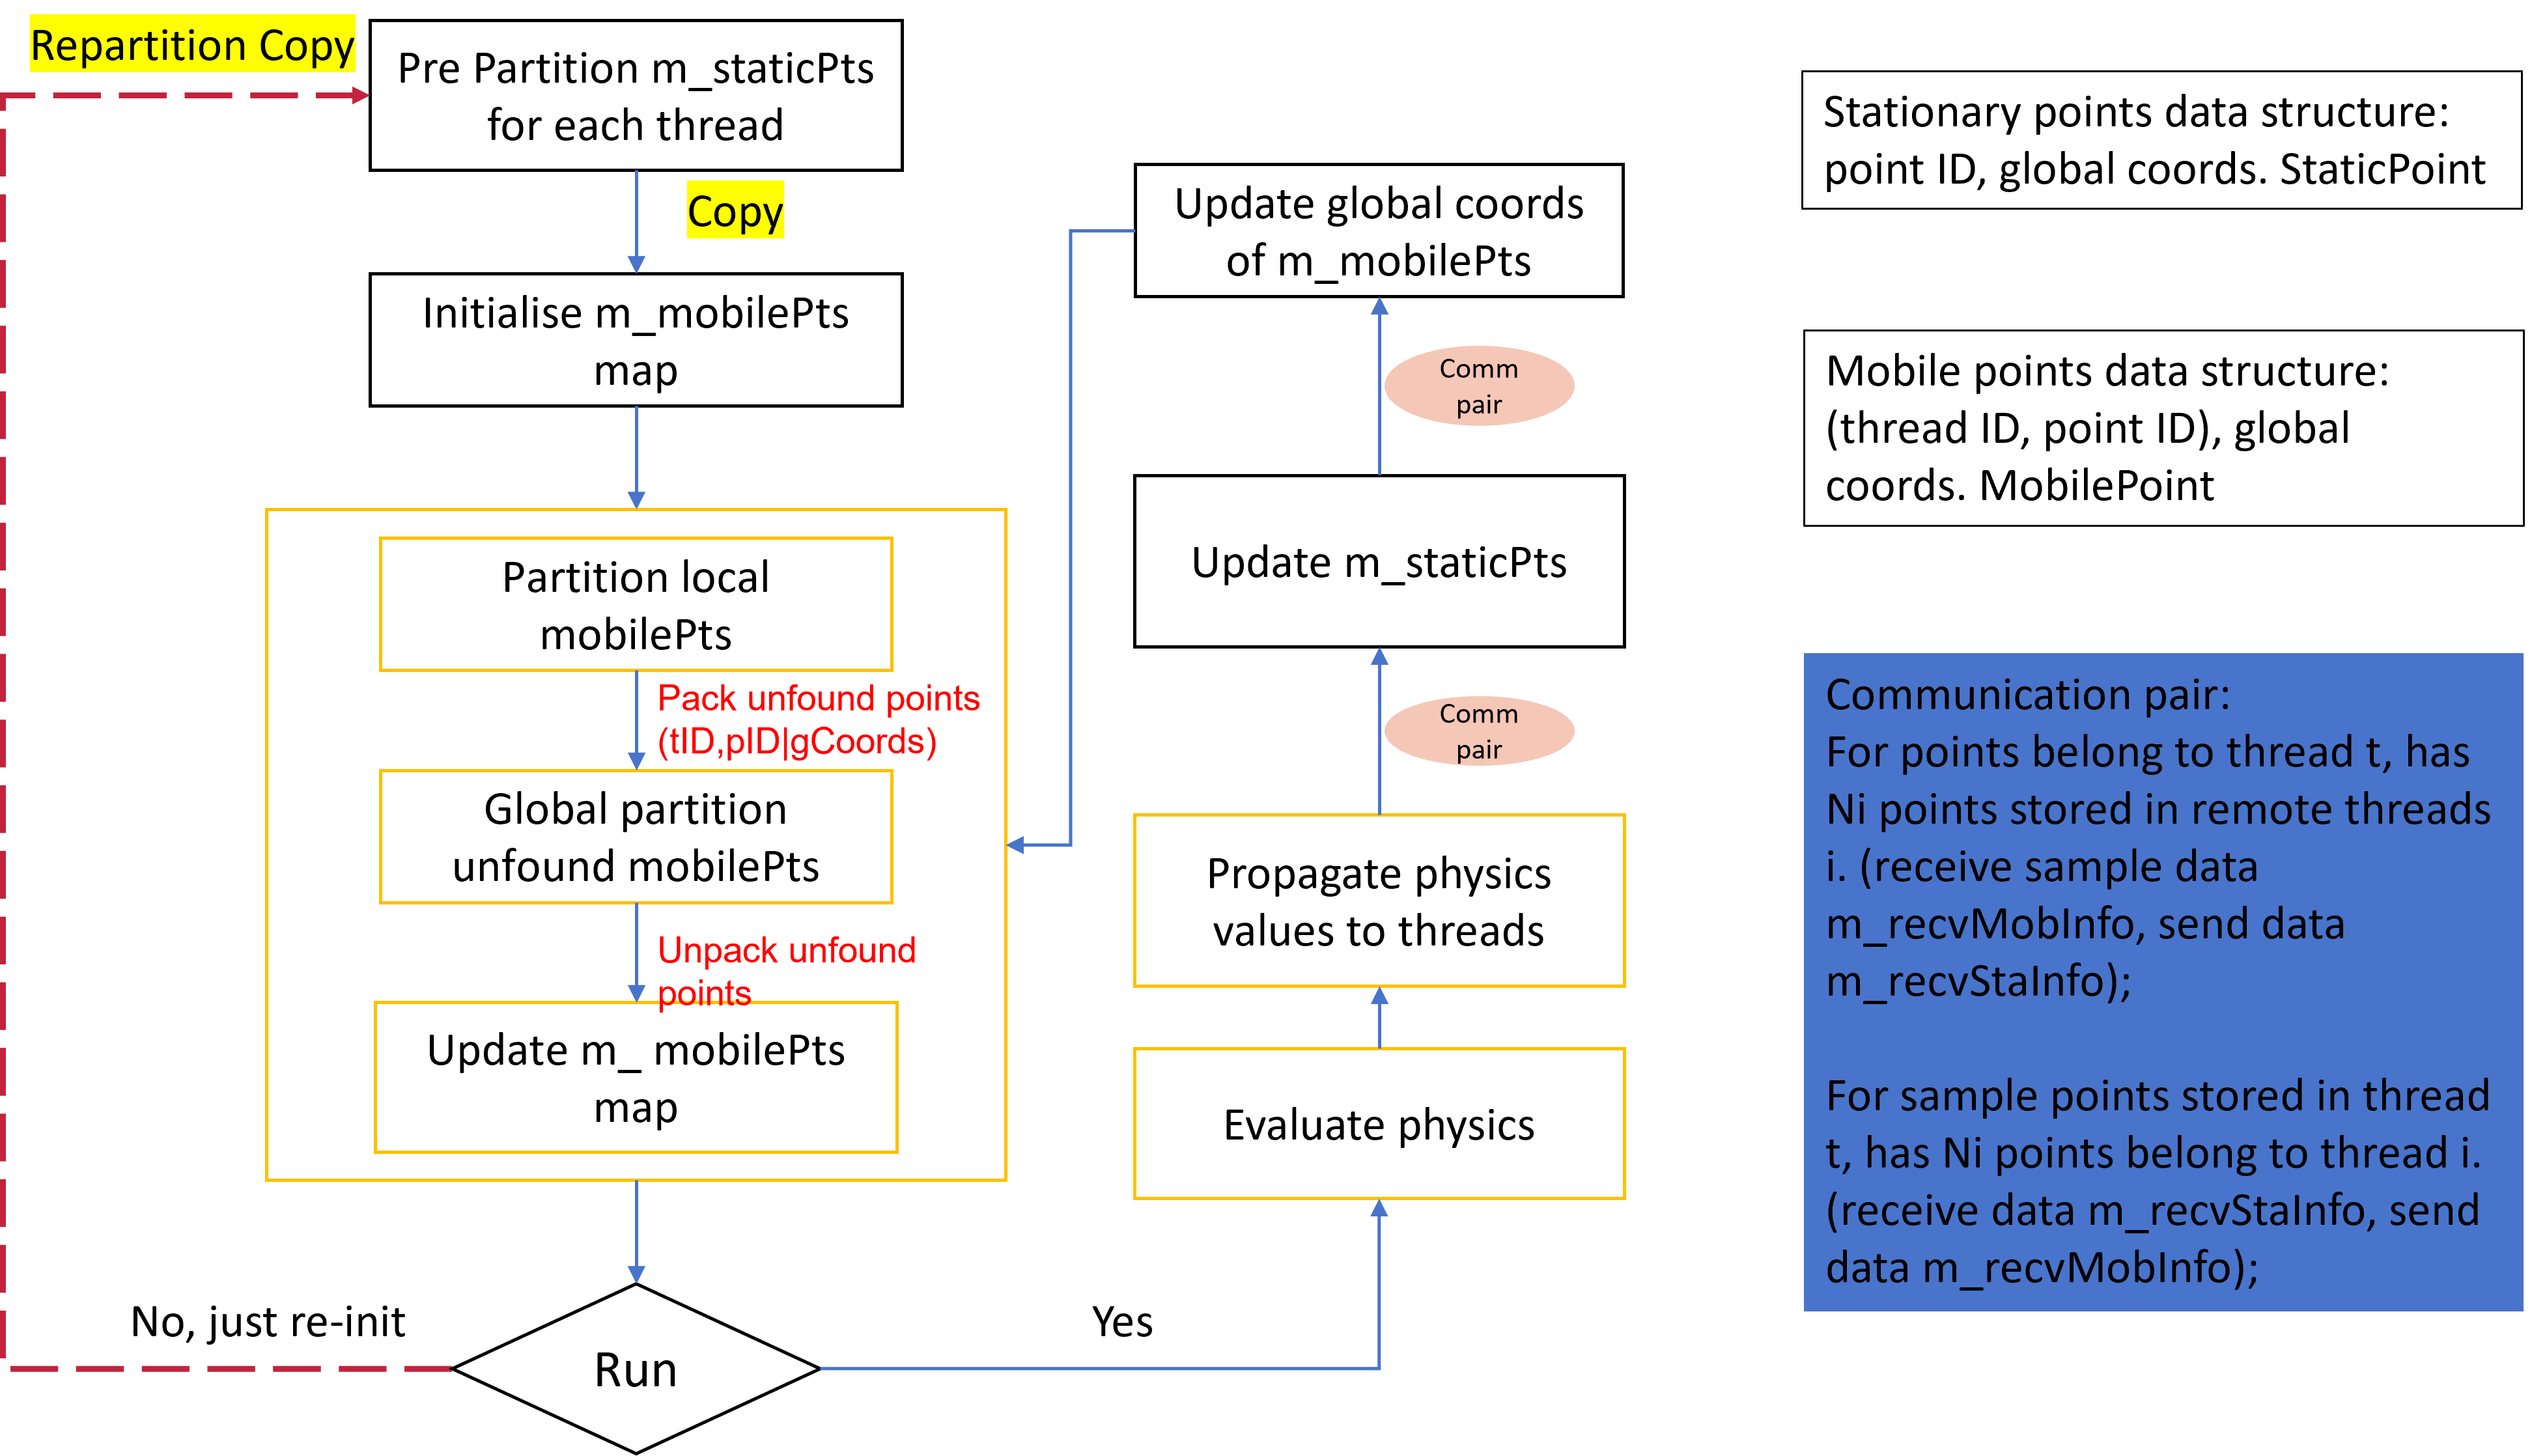
\includegraphics[width=\linewidth]{library/SolverUtils/img/LagrangianPtsTracking.png}
    \label{fig:LagrangianTrack}
    \caption{Design of the \texttt{FilterLagrangianPoints} class} 
\end{figure}


